%
% Exemplo LaTeX de artigo UNISINOS
%
% Elaborado com base nas orientações dadas no documento
% ``GUIA PARA ELABORAÇÃO DE TRABALHOS ACADÊMICOS''
% disponível no site da biblioteca da Unisinos.
% http://www.unisinos.br/biblioteca
% 
% Os elementos textuais abaixo são apresentados na ordem em que devem
% aparecer no documento.  Repare que nem todos são obrigatórios - isso
% é devidamente indicado em cada caso.
%
% Comentários abaixo colocados entre aspas (`` '') foram
% extraídos diretamente do documento da biblioteca.
%
% Este documento é de domínio público.
%

%=======================================================================
% Declarações iniciais identificando a classe de documento e
% selecionando alguns pacotes adicionais.
%
% As opções disponíveis (separe-as com vírgulas, sem espaço) são:
% - twoside: Formata o documento para impressão frente-e-verso
%   (o default é somente-frente)
% - english,brazilian,french,german,etc.: idiomas usados no documento.
%   Deve ser colocado por último o idioma principal.
%=======================================================================
\documentclass[english,brazilian]{UNISINOSartigo} %twoside
\usepackage[utf8]{inputenc} % charset do texto (utf8, latin1, etc.)
\usepackage[T1]{fontenc} % encoding da fonte (afeta a sep. de sílabas)
\usepackage{graphicx} % comandos para gráficos e inclusão de figuras
\usepackage{bibentry} % para inserir refs. bib. no meio do texto
\usepackage{float}
\usepackage{array}
\usepackage{tabularx}
\usepackage{booktabs}
\usepackage{multirow}
\usepackage{newfloat}
\usepackage{setspace}
\usepackage{enumitem}
\usepackage{placeins}
\usepackage{listings}
\usepackage{xcolor}

\lstdefinelanguage{JavaScript}{
  keywords={break, case, catch, class, const, continue, debugger, default, delete, do, else, export, extends, finally, for, function, if, import, in, instanceof, let, new, return, super, switch, this, throw, try, typeof, var, void, while, with, yield},
  morekeywords={async, await},
  sensitive=true,
  comment=[l]{//},
  morecomment=[s]{/*}{*/},
  string=[b]",
  morestring=[b]'
}

\lstset{
  language=JavaScript,
  basicstyle=\ttfamily\small,
  keywordstyle=\color{blue}\bfseries,
  commentstyle=\color{green!50!black}\itshape,
  stringstyle=\color{red},
  numbers=left,
  numberstyle=\tiny,
  stepnumber=1,
  numbersep=5pt,
  showstringspaces=false,
  breaklines=true,
  frame=single,
  captionpos=b
}

\newcommand{\lstcaptioncustom}[2][]{%
  \captionsetup{type=figure} % ou table se preferir
  \lstset{style=jsstyle, caption={#2}}%
  \lstinputlisting[#1]{#2}%
}

\setlength{\fboxsep}{1pt}
\setlength{\fboxrule}{0.5pt}
%\usepackage{longtable}

\DeclareFloatingEnvironment[
fileext=loq,
listname={Lista de Quadros},
name=Quadro,
%placement=p,
%within=section,
%chapterlistsgaps=off
]{quadro}

\newcolumntype{L}{>{\centering\arraybackslash}m{6.2cm}}
\newcolumntype{G}{>{\centering\arraybackslash}m{5.5cm}}
\newcolumntype{A}{>{\centering\arraybackslash}m{2.4cm}}
\newcolumntype{B}{>{\centering\arraybackslash}m{7.5cm}}
%=======================================================================
% Escolha do sistema para geração de referências bibliográficas.
%
% O default é usar o estilo unisinos.bst.  Comente a definição abaixo
% e descomente a linha seguinte para usar o estilo do ABNTeX (é
% necessário ter esse pacote instalado).
%
% A vantagem do unisinos.bst é que ele permite o uso de um arquivo .bib
% seguindo as orientações tradicionais do BibTeX (veja essas orientações
% em http://ctan.tug.org/tex-archive/biblio/bibtex/contrib/doc/btxdoc.pdf).
% Entretanto, o estilo não suporta algumas citações mais exóticas como
% apud.  Para isso, use o ABNTeX, mas esteja ciente de que muitas de
% suas referências serão incompatíveis com os estilos tradicionais do
% BibTeX como plain, alpha, ieeetr, entre outros.
%=======================================================================
\usepackage[alf]{abntex2cite}

\autor{CLOSS FRAGA}{GUILHERME}
\titulo{Inteligência Artificial e \textit{Vibe Coding} no Processo de Desenvolvimento de \textit{Software}:}
\subtitulo{Um estudo comparativo entre desenvolvedores com e sem o uso de ferramentas de IA}
\orientador[Prof.ª Dra.]{Francisco}{Rosemary}
%\coorientador[Prof.~Dr.]{Lamport}{Leslie}
\local{São Leopoldo}
\ano{2025}
\unidade{Unidade Acadêmica de Graduação}
\curso{Curso de Bacharelado em Ciência da Computação}
\natureza{%
Artigo apresentado como requisito parcial para obtenção do título de Bacharel em Ciência da Computação, pelo Curso de Ciência da Computação da Universidade do Vale do Rio dos Sinos (UNISINOS)}

%=======================================================================
% Início do documento.
%=======================================================================

\begin{document}
\capa
\folhaderosto

% Diferentemente do normal, os comandos a seguir devem vir aqui mesmo,
% e não antes do \begin{document} onde seria o lugar deles. 
\tituloArtigo{Inteligência Artificial e \textit{Vibe Coding} no Processo de Desenvolvimento de \textit{Software}:}{Um estudo comparativo entre desenvolvedores com e sem o uso de ferramentas de IA}
\autorArtigo{Guilherme Closs Fraga\footnote{Graduando em Ciência da Computação pela Unisinos. Email: guifraga8@edu.unisinos.br}}
\autorArtigo{Rosemary Francisco\footnote{Doutora em Administração. Email: rosemaryf@unisinos.br}}

%=======================================================================
% Resumo em Português.
%
% A recomendação é para 150 a 250 palavras.
%=======================================================================
\begin{abstract}
Este trabalho investiga a influência de ferramentas de Inteligência Artificial (IA) Generativa no processo de desenvolvimento de \textit{software}, analisando seu impacto na produtividade e eficiência de desenvolvedores. Foi conduzido um experimento comparativo entre dois grupos: um com acesso a ferramentas de IA e outro sem esse recurso, ambos submetidos a um mesmo desafio técnico de programação. Para isso, desenvolveu-se uma plataforma \textit{web} que permitiu o controle das etapas do experimento, coleta automática dos tempos de execução e envio das soluções. Os resultados demonstraram que o grupo que utilizou IA apresentou uma redução significativa no tempo médio de conclusão do desafio, embora nem todos os participantes tenham alcançado total correção da solução. Observou-se que o uso consciente e criterioso da IA contribui para a otimização do trabalho sem comprometer o raciocínio lógico do desenvolvedor. Conclui-se que as ferramentas de IA Generativa, quando aplicadas de forma estratégica, representam um apoio valioso no desenvolvimento de \textit{software}, potencializando a produtividade e reduzindo o tempo de entrega, mas ainda exigem análise crítica e validação humana para garantir a qualidade das soluções.
\palavraschave{inteligência artificial. IA generativa. desenvolvimento de software. produtividade. vibe coding.}
\end{abstract}

\begin{otherlanguage}{english}
\singlespacing
\begin{abstract}
This study investigates the influence of Generative Artificial Intelligence (AI) tools on the software development process, analyzing their impact on developer productivity and efficiency. A comparative experiment was conducted between two groups: one with access to AI tools and another without, both subjected to the same technical programming challenge. To support the experiment, a web platform was developed to manage the execution stages, automatically record completion times, and collect submitted solutions. The results showed that the group using AI achieved a significant reduction in the average completion time of the challenge, although not all participants reached full correctness in their solutions. It was observed that conscious and critical use of AI contributes to workflow optimization without compromising developers’ logical reasoning. The study concludes that Generative AI tools, when applied strategically, represent a valuable aid in software development by enhancing productivity and reducing delivery time, yet still require human oversight and validation to ensure the quality of outcomes.
\end{abstract}
\palavraschave{artificial intelligence. generative AI. software development. productivity. vibe coding.}
\end{otherlanguage}

%=======================================================================
% Introdução
%=======================================================================
\section{Introdução}

A Inteligência Artificial (IA) é considerada uma das tecnologias mais transformadoras da atualidade, impulsionando mudanças em diversos setores e despertando interesse tanto no meio acadêmico quanto no mercado \cite{machucho2025}. Trata-se do uso de algoritmos e modelos computacionais capazes de realizar tarefas tradicionalmente dependentes da cognição humana, como análise de dados, raciocínio lógico e tomada de decisão \cite{norvig2021}. Segundo relatório de \citeonline{deniz2023}, a utilização de ferramentas de IA generativa pode aumentar a produtividade de desenvolvedores em tarefas de codificação, permitindo a execução de certas atividades até duas vezes mais rápido que processos totalmente manuais. Apesar desses avanços, a adoção dessas tecnologias levanta questões sobre dependência excessiva, erosão de habilidades humanas e confiabilidade das soluções geradas.

No contexto do desenvolvimento de \textit{software}, a presença da IA tem se tornado particularmente evidente. Ferramentas que combinam aprendizado de máquina e processamento de linguagem natural auxiliam desenvolvedores em diversas etapas do ciclo de vida do \textit{software}, desde a escrita de código até a detecção de falhas e a otimização de desempenho \cite{coutinho2024}. Um exemplo é o \textit{GitHub Copilot}, lançado em 2021 pela \textit{GitHub} em parceria com a \textit{OpenAI}, que utiliza modelos de IA Generativa (também chamadas de IA Gen) para sugerir trechos de código em tempo real \cite{github2021}. Da mesma forma, agentes de codificação baseados em IA, alinhados ao conceito de \textit{vibe coding}, permitem que o desenvolvedor interaja de forma mais conversacional com a ferramenta, gerando código de maneira assistida, mas ainda mantendo controle sobre decisões críticas \cite{delaney2025}. Essas práticas têm sido discutidas como um avanço na programação assistida, trazendo benefícios de produtividade e colaboração entre humano e máquina.

Esses recursos, ao mesmo tempo em que oferecem praticidade e aumentam a produtividade, também levantam debates relevantes. Há questionamentos sobre até que ponto a utilização de IA generativa pode impactar o desenvolvimento de habilidades de raciocínio lógico e resolução de problemas, uma vez que o programador pode se tornar excessivamente dependente da ferramenta \cite{verastegui2025}. Além disso, o código gerado pode apresentar erros lógicos, violações de boas práticas e vulnerabilidades de segurança, exigindo revisão crítica por parte do profissional \cite{idrisov2024, tosi2024}. Estudos experimentais indicam resultados variados: enquanto tarefas simples podem ser concluídas significativamente mais rápido com IA, contextos complexos podem exigir maior tempo de revisão e adaptação do código \cite{peng2023, exame2025}.

Por outro lado, pesquisas recentes indicam que a adoção de IA no desenvolvimento de \textit{software} pode representar ganhos significativos em termos de produtividade e redução do tempo necessário para a entrega de soluções. Um estudo piloto com profissionais de \textit{software} demonstrou percepções majoritariamente positivas quanto ao impacto desses recursos na produtividade individual \cite{coutinho2024}. Essa realidade torna essencial a investigação de como essas ferramentas impactam o trabalho de desenvolvedores em contextos práticos. Assim, mais do que um recurso de conveniência, a IA se apresenta como um instrumento que pode redefinir processos e metodologias de engenharia de \textit{software}.

Diante desse cenário, torna-se essencial investigar como a IA Generativa influencia o desempenho de desenvolvedores. Este trabalho propõe um estudo comparativo entre dois grupos de participantes: um com acesso a ferramentas de IA Generativa e outro sem acesso a esses recursos, aplicando um desafio técnico de programação. O objetivo é avaliar variáveis como eficiência, tempo de resolução e capacidade para solucionar os problemas propostos, fornecendo uma investigação sobre vantagens e limitações do uso dessas tecnologias.

Assim, o objetivo geral desta pesquisa é analisar o uso de ferramentas de IA Generativa no Desenvolvimento de \textit{Software} por meio de um desafio técnico comparativo entre desenvolvedores com e sem acesso a essas ferramentas. A questão de pesquisa que orienta este estudo é: de que maneira o uso de ferramentas de IA Generativa contribui ou afeta o desempenho de desenvolvedores em atividades práticas de programação? Destacam-se também os objetivos específicos necessários para atingir a conclusão deste trabalho, sendo eles:

\begin{enumerate}[label=\alph*), leftmargin=1.2cm, itemsep=0.1em, topsep=0.1em]
    \item desenvolver uma plataforma \textit{web} simples para disponibilização do desafio técnico e coleta de dados de desempenho dos participantes;
    \item aplicar o desafio técnico a dois grupos de desenvolvedores, sendo um autorizado a utilizar ferramentas de IA e outro restrito ao uso dessas tecnologias;
    \item comparar os resultados obtidos pelos grupos em relação ao tempo de conclusão e resolução do desafio proposto;
    \item analisar as vantagens, limitações e possíveis implicações do uso de ferramentas de IA no processo de desenvolvimento de \textit{software}.
\end{enumerate}

As seções seguintes deste documento estão dispostas da seguinte forma: a segunda seção contempla a fundamentação teórica do trabalho, que discorre sobre o desenvolvimento de \textit{software} e IA Generativa aplicada ao desenvolvimento de \textit{software} propriamente. A terceira seção apresenta os trabalhos relacionados a esta pesquisa e uma breve comparação entre os mesmos. Na quarta seção apresenta-se a metodologia do trabalho, descrevendo como foi conduzida todas as etapas e elaborações da pesquisa. Na quinta seção está a proposta de modelo do trabalho, apresentando brevemente a arquitetura da plataforma, tecnologias utilizadas e seu fluxo de uso do lado dos participantes. Na sexta seção apresenta-se os resultados e discussões após coleta de dados por meio do experimento aplicado como um todo.

Por fim, ao fechamento do trabalho na última seção, encontra-se as conclusões e considerações finais levantadas com o experimento, assim como apontamentos para trabalhos futuros. Espera-se que os resultados forneçam evidências consistentes para compreender o papel da IA como aliada no processo de desenvolvimento de \textit{software}, oferecendo resultados para pesquisadores, profissionais e instituições interessadas em compreender e orientar o uso dessas ferramentas emergentes.

\section{Fundamentação Teórica}

Com base na temática que o presente trabalho visa abordar, se faz necessário discorrer sobre dois tópicos fundamentais para a construção e consolidação do mesmo, sendo eles: Desenvolvimento de \textit{Software} e IA Generativa aplicada ao desenvolvimento de \textit{software}. Nas seções seguintes, os conceitos são explorados e detalhados a fim de estabelecer os fundamentos teóricos necessários para compor este trabalho.

\subsection{Desenvolvimento de \textit{Software}}

Um \textit{software} refere-se a todos os componentes não físicos de um computador, redes de computadores ou dispositivos móveis. Em linhas gerais, refere-se aos programas e aplicações, como o próprio sistema operacional, que fazem aquele aparelho (ou ferramenta) operar de acordo com o que o usuário necessita. Isto é, \textit{software} se trata de uma coleção de instruções, dados ou programas utilizados para operar computadores e executar determinadas tarefas \cite{coutinho2021}.

Em outras palavras, pode-se dizer que é um termo genérico que se refere à aplicações, \textit{scripts} e programas executáveis em um determinado dispositivo. Assim, o diferencia de \textit{hardware}, que descreve os aspectos físicos de um aparelho. Sendo assim, pode-se estabelecer o \textit{software} como um componente variável de um computador, enquanto o \textit{hardware} é constante \cite{sakurai2018}

De acordo com \citeonline{maynard2015}, existem basicamente dois tipos de \textit{software}, sendo eles: \textit{software} de aplicativo e \textit{software} de sistema. Um aplicativo seria aquele que atende uma necessidade específica ou executa determinadas tarefas. E, segundo \citeonline{schwab2019}, \textit{software} de sistema seria a parte essencial para que o \textit{hardware} de um computador opere, servindo como a plataforma para a execução de aplicativos. Ademais, pode-se mencionar outros tipos de \textit{software}, como os de programação, que são ferramentas necessárias para desenvolvedores, \textit{middlewares}, responsáveis por atuarem entre o \textit{software} do sistema e aplicativos e até mesmo \textit{drivers}, que são responsáveis por operarem dispositivos e periféricos de computadores.

Por fim, a sincronia entre diferentes tipos de \textit{software} e \textit{hardware}, é peça fundamental para o funcionamento eficiente de sistemas computacionais. Enquanto um aplicativo permite que seus usuários realizem determinadas tarefas, um sistema assegura que o \textit{hardware} opere corretamente, dando suporte para diferentes aplicações. Com a constante crescente de complexidade em sistemas modernos, a presença de um \textit{middleware} eficaz se torna indispensável para assegurar que diferentes \textit{softwares} funcionem em harmonia. Da mesma forma que, \textit{drivers} são indispensáveis para comunicação entre o sistema e periféricos, o que amplia as funcionalidades de um computador, resultando na melhoria da experiência do usuário.

Os \textit{softwares}, diferentemente do hardware, não são tangíveis e representam os componentes lógicos responsáveis pelo funcionamento de um computador ou dispositivo móvel. De acordo com \citeonline{candido2022}, o sistema operacional constitui o software fundamental, sendo exemplos mais conhecidos o \textit{Windows}, \textit{macOS} e \textit{Linux}, que variam em suas interfaces de usuário. Além dele, outros programas complementam as funções básicas, como o \textit{Microsoft Office} e o \textit{MediaPlayer} \cite{neto2019}, além de \textit{softwares} utilitários, como antivírus, ferramentas de \textit{backup} e manutenção de disco, que garantem desempenho e segurança. O avanço tecnológico também possibilitou o surgimento da virtualização, permitindo a execução de diferentes sistemas operacionais em uma única máquina física e ampliando a flexibilidade no uso dos recursos.

O \textit{software} pode ainda estar integrado diretamente ao \textit{hardware}, como em painéis eletrônicos de automóveis ou leitores de \textit{Blu-Ray}, caracterizando os chamados “embutidos” \cite{coutinho2021}. Historicamente, \textit{software} e \textit{hardware} eram concebidos como uma única unidade, sendo o termo “\textit{software}” empregado pela primeira vez por John W. Tukey em 1958 \cite{maynard2015}. Somente vinte anos depois, o governo dos Estados Unidos determinou que a IBM passasse a contabilizar \textit{hardware} e \textit{software} separadamente, o que abriu espaço para empresas especializadas \cite{sakurai2018}. Essa dissociação entre \textit{hardware} e \textit{software} impulsionou a inovação, permitindo atualizações independentes, acelerando ciclos de desenvolvimento e fomentando novos modelos de negócio baseados em \textit{software}, que hoje ocupam posição central na economia digital.

\citeonline{schwab2019} destaca que o trabalho do programador consiste, de forma essencial, em traduzir requisitos e algoritmos para uma linguagem de programação que o computador consiga interpretar e executar. A partir desse processo, é possível desenvolver diferentes tipos de \textit{software}, como aplicativos, jogos e sistemas de controle para robôs. Um exemplo histórico ligado à ideia de programação foi a invenção de um \textit{tear} “programável” pelo francês Joseph-Marie Jacquard, que representou um marco na Revolução Industrial. O equipamento não possuía processador, sendo controlado por meio de cartões perfurados. Conforme explica \citeonline{maynard2015}, esses cartões não utilizavam valores binários como 0 e 1, mas funcionavam através da presença ou ausência de perfurações: um furo indicava uma ação de movimento, enquanto a ausência significava outra. A criação de Jacquard é considerada uma das precursoras da automação moderna.

\citeonline{maynard2015} aponta que, em 1843, Augusta Ada King-Noel, mais conhecida como Ada Lovelace, desempenhou um papel marcante ao colaborar com Charles Babbage no projeto do \textit{Analytical Engine}, uma calculadora mecânica de uso geral que acabou não sendo concluída. Durante esse processo, Ada elaborou diversas anotações e descreveu um método para calcular os números de Bernoulli por meio da máquina, o que, segundo \citeonline{coutinho2021}, é considerado o primeiro programa de computador da história. Posteriormente, em 1941, Konrad Ernst Otto Zuse desenvolveu o Z3, reconhecido como o primeiro sistema de computação totalmente automatizado e programável do mundo.

O Z3 foi construído a partir dos conceitos idealizados por Babbage e tinha como diferencial a capacidade de realizar operações, como a adição, em menos de um quarto de segundo. O propósito central de sua criação estava ligado à busca por maior eficiência nos cálculos. Nos primeiros anos, os \textit{softwares} eram desenvolvidos para máquinas específicas e eram comercializados em conjunto com o \textit{hardware}. Já na década de 1980, passaram a ser distribuídos em mídias físicas, como disquetes, e mais tarde em CDs e DVDs. Atualmente, grande parte dos \textit{softwares} é obtida por meio da \textit{Internet}, seja diretamente nos sites dos fabricantes ou através de plataformas de distribuição de aplicativos.

Os modelos de ciclo de vida de \textit{software} descrevem as etapas que um sistema percorre desde sua concepção até sua desativação, organizando a sequência de atividades necessárias para o desenvolvimento. O objetivo central desses modelos é garantir qualidade, reduzir custos e otimizar o tempo de entrega. Entre as fases mais comuns estão:

\begin{itemize}[leftmargin=1cm, itemsep=0.1em, topsep=0.1em]
    \item Análise de Requisitos: onde são levantadas e documentadas as necessidades do sistema;
    \item Design: define a arquitetura, fluxos de trabalho e tecnologias a serem utilizadas;
    \item Implementação: fase em que o código é desenvolvido com base no planejamento estabelecido;
    \item Testes: que envolvem diferentes tipos de verificação para assegurar a confiabilidade do \textit{software};
    \item Manutenção: responsável por corrigir falhas e implementar melhorias após a entrega do sistema. 
\end{itemize}

De acordo com \citeonline{candido2022}, observa-se nos últimos anos uma tendência de desprofissionalização no aprendizado de programação, já que muitas pessoas têm adquirido essas habilidades de forma autodidata, recorrendo a tutoriais \textit{online} em vez de cursos formais. Além disso, o \textit{networking} global, aliado às diversas plataformas digitais, tem favorecido a formação de grandes comunidades que reúnem tanto entusiastas quanto programadores experientes, tornando cada vez menos nítida a distinção entre esses grupos.

Ao mesmo tempo, percebe-se um avanço significativo nos padrões e na qualidade do desenvolvimento de \textit{software}. Os sistemas estão cada vez mais sofisticados e complexos, o que aumenta a demanda por soluções digitais. Esse contexto reflete uma sociedade em constante transformação, onde as necessidades mudam rapidamente, gerando uma procura crescente por Desenvolvedores \textit{Full Stack} (um profissional de tecnologia que possui a capacidade de trabalhar em todas as camadas de um projeto de \textit{software}) em detrimento de profissionais especializados apenas em uma área.

A complexidade crescente dos sistemas requer profissionais capazes de atuar em todas as camadas do desenvolvimento, abrangendo desde o \textit{Frontend} (interface do usuário) até o \textit{Backend} (servidor, banco de dados e lógica de negócios de uma aplicação). Nesse cenário, os Desenvolvedores \textit{Full Stack} ganham destaque por sua flexibilidade e capacidade de adaptação às mudanças do mercado e às demandas dos usuários. Sua habilidade em compreender e integrar diferentes componentes de um sistema favorece um desenvolvimento mais unificado e eficiente, além de melhorar a comunicação e colaboração dentro das equipes. Assim, em um ambiente em que a agilidade e a adaptabilidade são fatores essenciais, esses profissionais se consolidam como recursos estratégicos para empresas que buscam manter a competitividade.

O desenvolvimento de \textit{software} pode ser entendido como um conjunto de atividades voltadas ao projeto, criação, implementação e manutenção de programas que orientam o funcionamento de computadores, sendo independente do \textit{hardware} e responsável por torná-los programáveis \cite{schwab2019}.

Conforme aponta \citeonline{candido2022}, o desenvolvimento de \textit{software} deve ser integrado ao desenvolvimento de produtos mecânicos e elétricos, o que faz com que o papel dos desenvolvedores de \textit{software} seja menos delimitado em comparação ao dos engenheiros. Esses profissionais podem focar em áreas específicas do projeto, como a codificação, enquanto o ciclo de vida do \textit{software} envolve a transformação de requisitos em funcionalidades, o trabalho em equipes multifuncionais, a gestão de processos e equipes, além de atividades de teste e manutenção.

De acordo com \citeonline{schwab2019}, a atuação dos desenvolvedores de \textit{software} vai além das equipes de programação, envolvendo também cientistas e fabricantes de dispositivos e \textit{hardware}, que contribuem para a criação de códigos, mesmo não sendo os principais responsáveis pelo desenvolvimento. Essa participação não se limita às indústrias tradicionais de tecnologia da informação, abrangendo também empresas que não se dedicam exclusivamente à produção de \textit{software} ou semicondutores.

A ampliação do papel dos desenvolvedores de \textit{software} evidencia a crescente integração da tecnologia da informação com diversas áreas, como ciência, medicina, engenharia e artes. Atualmente, o desenvolvimento de \textit{software} é fundamental para múltiplos setores, desde a indústria automotiva até o entretenimento, impulsionando a inovação e a transformação digital. Na indústria automotiva, esses profissionais são essenciais para o desenvolvimento de sistemas de condução autônoma e tecnologias avançadas de segurança. Já no cinema, os efeitos visuais e a animação digital dependem fortemente do \textit{software} para criar mundos e personagens realistas. Dessa forma, os desenvolvedores de \textit{software} exercem um papel cada vez mais diversificado e influente, moldando o futuro em diferentes áreas do conhecimento e da atividade humana.

\subsubsection{Modelos de Desenvolvimento de \textit{Software}}

O desenvolvimento de \textit{software} pode ser conduzido por diferentes abordagens, conhecidas como modelos de processo de \textit{software}. Esses modelos têm como objetivo estruturar e organizar as atividades necessárias para transformar requisitos em um produto final de qualidade. Existem diversos modelos conhecidos, entretanto, os mais populares e utilizados acabam sendo o Modelo Cascata e os Modelos Ágeis.

O Modelo Cascata (ou \textit{Waterfall}), proposto por Winston Royce em 1970, é um dos primeiros modelos formais de processo de \textit{software} e segue uma sequência linear de fases: levantamento de requisitos, análise, projeto, implementação, testes, implantação e manutenção. Cada fase deve ser concluída antes do início da próxima, funcionando como uma “cascata” de atividades \cite{sommerville2011}. Sua estrutura é simples e fácil de entender, com definição clara das fases e entregas, sendo útil em projetos com requisitos bem definidos e estáveis. No entanto, apresenta pouca flexibilidade diante de mudanças nos requisitos, pode identificar falhas tardiamente, geralmente na fase de testes, e tem dificuldade em lidar com projetos complexos ou inovadores.

Os Modelos Ágeis surgiram como alternativa aos modelos tradicionais, formalizados em 2001 com o Manifesto Ágil \cite{beck2001}. Eles priorizam a colaboração com o cliente, entregas rápidas e contínuas, adaptação às mudanças e interações entre pessoas mais do que processos rígidos. Entre os métodos ágeis mais utilizados estão \textit{Scrum}, \textit{Kanban} e \textit{Extreme Programming} (conhecido também como \textit{XP}), que dividem o projeto em pequenas iterações (ciclos), resultando em entregas frequentes e incrementais. Esses modelos oferecem alta flexibilidade para mudanças de requisitos, entregas rápidas que geram valor contínuo ao cliente e melhoram a comunicação e colaboração entre equipe e \textit{stakeholders}. Por outro lado, podem gerar falta de documentação formal, exigem alto envolvimento do cliente e são menos indicados para projetos de missão crítica que demandam forte rastreabilidade.

Sendo assim, evidencia-se que cada modelo de desenvolvimento possui suas características, vantagens e limitações. A escolha do modelo mais adequado depende do contexto do projeto, da complexidade do sistema, do nível de risco, do grau de inovação e da estabilidade dos requisitos. Modelos tradicionais como Cascata são mais estruturados, os modelos Ágeis oferecem maior flexibilidade e adaptabilidade, características cada vez mais valorizadas no mercado atual. Na Tabela \ref{tab:modelosDev}, temos um comparativo resumido dos principais pontos dos modelos citados.

\begin{table}[ht]
    \caption{Comparativo entre Modelo Cascata e Modelos Ágeis}
    \label{tab:modelosDev}
    \centering%
    \footnotesize
    \begin{tabularx}{\textwidth}{lXXXX}
        \toprule
        \textbf{Modelo} & \textbf{Resumo} & \textbf{Vantagem} & \textbf{Desvantagem} & \textbf{Indicado para}\\
        \midrule
        Cascata & Linear e sequencial & Simples e claro & Pouca flexibilidade & Projetos pequenos e estáveis \\
        \midrule
        Ágeis & Iterativo e adaptável & Entregas rápidas & Pouca documentação & Projetos dinâmicos e mutáveis \\
        \bottomrule
    \end{tabularx}
    \fonte{Elaborado pelo autor}
\end{table}
\FloatBarrier

\subsection{IA Generativa (aplicada ao desenvolvimento de \textit{software})}

A Inteligência Artificial (IA) consolidou-se como uma das áreas mais relevantes da Ciência da Computação, devido à sua capacidade de simular processos cognitivos humanos como aprendizagem, raciocínio e tomada de decisão por meio de algoritmos e modelos matemáticos. Nos últimos anos, a evolução tecnológica permitiu que esses sistemas ultrapassassem o campo do reconhecimento de padrões e da automação, alcançando um estágio em que são capazes de gerar novos conteúdos, fenômeno que deu origem ao conceito de Inteligência Artificial Generativa \cite{basic2024, sauvola2024}. A IA Generativa distingue-se de modelos meramente classificatórios ou preditivos, produzindo resultados originais, como textos, imagens, sons ou códigos, a partir da análise de grandes volumes de dados e \textit{prompts} em linguagem natural.

Historicamente, a IA aplicada ao desenvolvimento de \textit{software} concentrou-se na automação de tarefas repetitivas e no suporte à decisão de programadores \cite{velpucharla2025}. Com o avanço dos modelos generativos, surgiram assistentes capazes de escrever trechos de código, gerar documentação, criar testes automatizados e até propor refatorações de programas. Essa evolução, associada à popularização de modelos de linguagem de grande escala (\textit{Large Language Models} ou \textit{LLMs}), tem transformado a forma como os desenvolvedores interagem com os sistemas, promovendo o conceito de “\textit{vibe coding}”, em que a colaboração entre humano e máquina cria um fluxo contínuo de desenvolvimento mais eficiente \cite{song2025}.

No contexto prático, a IA Generativa tem demonstrado potencial para aumentar a produtividade e reduzir o tempo de entrega de soluções. Estudos indicam que, embora códigos gerados automaticamente sejam adequados para tarefas de baixa complexidade, apresentam limitações quando aplicados a problemas que exigem conhecimento de domínio ou integração com sistemas legados \cite{liu2024}. De forma semelhante, \citeonline{yu2025} evidenciou que ferramentas como \textit{Codeium} e \textit{GitHub Copilot} melhoram a eficiência em atividades repetitivas, mas não substituem o conhecimento técnico aprofundado do programador. Estudos comparativos, como o de \citeonline{song2025}, indicam que essas ferramentas apresentam desempenho variável em critérios de correção, confiabilidade e manutenibilidade, funcionando melhor como apoio ao programador do que como substitutos plenos.

A segurança e a qualidade do código também são desafios significativos. \citeonline{shukla2025} destacam que a IA Generativa pode introduzir vulnerabilidades, erros sutis e inconsistências com padrões regulatórios e boas práticas de codificação. Essa necessidade de revisão crítica é corroborada por \citeonline{basic2024}, que enfatizam que a integração de IA no ciclo de desenvolvimento exige protocolos rigorosos de validação para assegurar a confiabilidade do \textit{software}. Além disso, a dependência excessiva de ferramentas generativas pode reduzir a prática de raciocínio lógico e resolução de problemas por parte dos desenvolvedores, criando um novo desafio educacional e profissional.

Questões éticas e sociais também ganham relevância nesse cenário. \citeonline{pant2024} destacam problemas relacionados à contextualização insuficiente do código, direitos autorais, privacidade e compromisso em sistemas críticos. Além disso, o fenômeno do \textit{vibe coding} levanta reflexões sobre como equilibrar a colaboração humano-máquina sem comprometer a autonomia e o aprendizado do programador \cite{song2025}. As organizações que adotam essas tecnologias precisam considerar políticas claras de governança, treinamento e avaliação contínua da eficácia das soluções geradas.

Em síntese, a IA Generativa aplicada ao desenvolvimento de \textit{software} apresenta grande potencial de inovação, automação e aumento de produtividade. No entanto, sua utilização requer acompanhamento crítico, validação constante do código produzido e reflexão sobre os impactos éticos, sociais e técnicos. A literatura indica que, embora essas ferramentas possam ser aliadas poderosas, elas não substituem o conhecimento humano, sendo mais eficazes quando integradas de forma complementar ao processo de desenvolvimento tradicional \cite{deniz2023, yu2025}.

\section{Trabalhos Relacionados}

Para fins de melhor localizar os trabalhos com temáticas relacionadas para o presente estudo, foi utilizado a plataforma de busca especializada em literatura acadêmica e científica Google Scholar. Os procedimentos de pesquisa e seleção consistiram em utilizar palavras chaves em português como “inteligência artificial generativa”, “desenvolvimento de software”, “produtividade”, “suporte”, “otimização” e “performance”, variando também os termos em inglês. Por fim, para selecionar os trabalhos a seguir, foi considerado o contexto do estudo de cada autor, conceitos abordados, tecnologias mencionadas e/ou utilizadas e problemáticas ressaltadas, que melhor correlacionassem com o presente estudo.

\subsection{Trabalhos Acadêmicos}

Dado o contexto do aprimoramento e evolução de Inteligências Artificiais Generativas nos anos recentes, tal como suas aplicabilidades para otimização de tarefas voltadas para a área de desenvolvimento de software, diversos estudos têm sido realizados com o intuito de explorar ainda mais os conceitos técnicos e práticos. A seguir, são apresentados estudos e pesquisas relacionados ao tema, estabelecendo um paralelo com a temática abordada para este trabalho.

\citeonline{gomes2023} apresenta uma análise comparativa de diferentes Inteligências Artificiais Generativas (IAs Generativas) aplicadas no desenvolvimento de software, mas particularmente focando em ferramentas auxiliares como \textit{GitHub Copilot}, \textit{Codeium}, \textit{Tabnine} e \textit{CodeGeeX}. Para fins práticos, seu trabalho focou em experimentos utilizando \textit{GitHub Copilot} e \textit{Codeium} para mensurar a eficiência das ferramentas.

Como resultado, o \citeonline{gomes2023} aponta que ambas as tecnologias se mostram extremamente úteis no processo de otimização do desenvolvimento, produtividade e qualidade de códigos, com a escolha entre elas dependendo das necessidades particulares do projeto e das preferências do profissional. Entretanto, o destaque ficou para a ferramenta \textit{GitHub Copilot}, que apresentou uma leve vantagem, com uma capacidade superior de compreensão para construção de uma lógica de desenvolvimento mais coesa.

Em \citeonline{daSilva2025}, é realizado o teste prático de viabilidade de desenvolvimento de uma aplicação \textit{web} para gerenciamento de sócios torcedores de um clube de futebol, utilizando IA Generativa como apoio na construção da aplicação. Ainda que, neste estudo os autores desenvolveram uma solução simples, utilizando tecnologias como \textit{JavaScript}\footnote{\textit{JavaScript}: \url{https://developer.mozilla.org/pt-BR/docs/Web/JavaScript}}, \textit{PHP}, \textit{HTML5} e entre outras, o trabalho demonstrou que utilizar de Inteligência Artificial otimiza o processo de desenvolvimento, desde a geração de código, identificação de falhas e sugestões de melhores práticas para a construção de soluções.

De acordo com os autores e os resultados obtidos \cite{daSilva2025}, a adoção de IA Generativa no processo de desenvolvimento contribui tanto para acelerar a produção, quanto para a qualidade e otimização da aplicação. Para o estudo em questão, os autores contaram com o suporte de modelos de IA Generativa como \textit{GPT-3.5} e \textit{Claude 1}.

Em contrapartida, no trabalho de \citeonline{ferreira2023}, o autor aborda sobre a influência das IAs Generativas na área de desenvolvimento de software, com base em um estudo qualitativo, combinando cenários exploratórios e descritivos. Aqui, o autor menciona o uso de ferramentas como o \textit{ChatGPT}, \textit{Bard}, \textit{GitHub Copilot} para tratar sobre a temática de modelos baseados no conceito de Processamento de Linguagem Natural (PLN).

Ao longo de seu estudo, \citeonline{ferreira2023} aborda questões como o impacto da Inteligência Artificial na programação, trazendo dados e referências, para dissertar sobre tópicos como os desafios e benefícios do uso de ferramentas de IA. Sobre os desafios, o autor menciona a questão da dependência do uso de IA, limitando assim o desenvolvimento de habilidades próprias por parte do programador e a substituição do desenvolvedor por IA, assunto fortemente debatido desde a evolução das IAs Generativas nos anos recentes. 

\citeonline{santos2024} investigou a influência das ferramentas de IA Generativas, citando \textit{ChatGPT} e \textit{GitHub Copilot}, com foco no processo de ensino e aprendizagem das instituições de ensino superior na área de desenvolvimento de \textit{software}. O objetivo deste estudo consistiu em identificar oportunidades e desafios no uso destas tecnologias. Para isso, o autor realizou um comparativo com grupos de alunos iniciantes, estagiários no setor de tecnologia, alocando-os em um projeto simulado.

Para tanto o autor \cite{santos2024} seguiu um delineamento \textit{crossover} 2x2 AB/BA, isto é, alternando os grupos entre o uso e não uso de IA. Após a coleta de dados, foi mensurado o conhecimento técnico dos grupos, tal como qualidade dos artefatos gerados, avaliação do produto desenvolvido e provas simuladas para testar o conhecimento adquirido. Aqui, o autor ressalta que os grupos que fizeram o uso de IA obtiveram melhores avaliações nos artefatos desenvolvidos, desde a documentação ao desenvolvimento de \textit{software} propriamente dito. Entretanto, a nível de conhecimento, não refletiu em avaliações melhores nas provas simuladas (notas de avaliações, propriamente).

\citeonline{costa2024} explorou como o uso de IA Generativa pode otimizar e aprimorar o processo de desenvolvimento de \textit{software} no contexto empresarial. O autor conduziu uma extensa revisão bibliográfica com o intuito de identificar as ferramentas e metodologias mais atuais e eficazes no mercado. A partir de então, selecionou e implementou \textit{frameworks} como \textit{Spring Boot} para a construção de uma aplicação escalável em \textit{Java}, utilizando o \textit{ChatGPT} como ferramenta de suporte durante o processo.

Ademais, o autor \cite{costa2024} fez o uso de ferramentas de teste e documentação de \textit{APIs}, tais como \textit{Postman} e até mesmo \textit{JUnit}, como \textit{framework} para validação de testes unitários. Em seu trabalho, o autor utilizou a IA Generativa através de \textit{prompts} para criação de todos os requisitos, códigos e validações do seu projeto. Como resultado, ele evidenciou uma melhoria na eficiência tanto do desenvolvimento quanto da qualidade da aplicação entregue. Entretanto, ressaltou a importância de que, o conhecimento prévio para uso de IAs Generativas é fundamental, para que se torne possível o uso da mesma como ferramenta de apoio no processo de desenvolvimento de \textit{software}.

Por fim, com base nos estudos analisados e considerando o crescimento acelerado das ferramentas de Inteligência Artificial Generativa na atualidade, evidencia-se que o profissional, independentemente da área de atuação, pode, e deve, tirar proveito dessas tecnologias para se manter em constante aprendizado e adaptado às novas realidades do mercado. Ou seja, não é necessário dominar todos os princípios técnicos por trás dessas ferramentas, mas sim saber utilizá-las estrategicamente, visando otimização, desempenho e melhores resultados.

Dessa forma, a proposta deste estudo é analisar, com base em dados e indicadores, o quanto o uso da Inteligência Artificial Generativa pode contribuir, junto aos profissionais da área de desenvolvimento de \textit{software}, para a entrega de soluções mais ágeis. Para delimitar o foco principal do trabalho, o segmento analisado será o desenvolvimento de software, considerando o papel do desenvolvedor no cenário atual do mercado de trabalho.

Com base no levantamento de todas as informações dos trabalhos relacionados ao tema, é possível agrupar as principais características de cada um deles para fins de comparação. Dada as informações levantadas, separa-se as características em quatro parâmetros, sendo eles:

\begin{itemize}[leftmargin=1cm, itemsep=0.1em, topsep=0.1em]
    \item  \textbf{Tema principal:} define qual foi o principal tema abordado ao longo do estudo;
    \item \textbf{Metodologia aplicada:} define o modelo utilizado para o estudo em questão;
    \item \textbf{Tecnologias/Inteligências Artificiais utilizadas:} se aplicável, define as ferramentas e/ou tecnologias utilizadas para fins de estudo, tal como o modelo de Inteligência Artificial utilizado ou analisado;
    \item \textbf{Objetivo:} define o objetivo do modelo, ou seja, qual problemática o modelo buscou esclarecer ao seu decorrer.
\end{itemize}

A partir do resultado do levantamento de trabalhos relacionados, foi possível elaborar a Tabela \ref{tab:estudos}, onde mostra o conteúdo dos critérios apontados em cada estudo, por ordem de apresentação.

\begin{table}[ht]
    \caption{Comparativo entre os trabalhos relacionados}
    \label{tab:estudos}
    \centering%
    \footnotesize
    \begin{tabularx}{\textwidth}{lXXXX}
        \toprule
        \textbf{Autores} & \textbf{Tema} & \textbf{Metodologia} & \textbf{Tecnologias/IA} & \textbf{Objetivo}\\
        \midrule
        \citeonline{gomes2023} & Comparação de IAs no desenvolvimento de \textit{software} & Testes práticos comparativos & \textit{GitHub Copilot}, \textit{Codeium}, \textit{Tabnine}, \textit{CodeGeeX} & Avaliar eficiência de ferramentas de IA no desenvolvimento \\
        \midrule
        \citeonline{daSilva2025} & Aplicação de IA na criação de sistemas \textit{web} & Estudo de caso com experimento & \textit{JavaScript}, \textit{PHP}, \textit{HTML5}, \textit{GPT-3.5}, \textit{Claude 1} & Verificar ganho de produtividade com uso de IA \\
        \midrule
        \citeonline{ferreira2023} & Impacto da IA na programação & Estudo qualitativo exploratório & \textit{ChatGPT}, \textit{Bard}, \textit{GitHub Copilot} & Analisar benefícios e riscos do uso da IA \\
        \midrule
        \citeonline{santos2024} & IA no ensino de tecnologia & Experimento com grupos (\textit{crossover}) & \textit{ChatGPT}, \textit{GitHub Copilot} & Medir impacto da IA na aprendizagem e desempenho técnico \\
        \midrule
        \citeonline{costa2024} & Uso de IA Generativa no desenvolvimento de \textit{software} empresarial & Revisão bibliográfica com aplicação prática & \textit{Spring Boot}, \textit{Java}, \textit{ChatGPT}, \textit{Postman}, \textit{JUnit} & Otimizar e melhorar eficiência e qualidade no desenvolvimento de aplicações \\
        \bottomrule
    \end{tabularx}
    \fonte{Elaborado pelo autor}
\end{table}
\FloatBarrier

\section{Materiais e Métodos}

Este trabalho tem como principal objetivo investigar a utilização de IA Generativa no processo de desenvolvimento de \textit{software}. A partir do conhecimento consolidado com base na fundamentação teórica, o presente estudo consiste em um breve experimento, dividido em dois grupos participantes do mesmo.

Sendo assim, para atingir os objetivos, a pesquisa percorreu cinco fases. A primeira consistiu em analisar trabalhos relacionados, almejando identificar tópicos existentes sobre o assunto ou que explorassem conceitos e práticas no que dizem respeito ao desenvolvimento de \textit{software} com auxílio de IA. Com base nesta análise, foi possível traçar um paralelo entre os estudos relacionados e o modelo proposto.

Na segunda fase, definiu-se as tecnologias, bem como a arquitetura da aplicação \textit{web} proposta para o desenvolvimento do trabalho. Com isso, estabelece-se o alicerce para o desenvolvimento da solução e para o cumprimento dos objetivos do trabalho.

A terceira fase consistiu no desenvolvimento da aplicação \textit{web} que foi utilizada como ambiente de execução do desafio técnico, assim como a elaboração do desafio disponibilizado dentro da plataforma. O objetivo central da ferramenta foi de oferecer, de forma prática e organizada, o enunciado do desafio, permitindo que os participantes iniciassem a atividade e, ao final, submetessem suas soluções. Além disso, a aplicação foi responsável por registrar automaticamente o tempo total despendido por cada participante, desde o momento em que iniciou a tarefa até a finalização do envio, viabilizando a coleta de dados confiáveis para a análise posterior.

A quarta fase compreendeu a aplicação prática do modelo e a coleta de dados. Para tanto, foram selecionados participantes por conveniência, ou seja, profissionais de desenvolvimento de \textit{software} previamente conhecidos pelo pesquisador e que se dispuseram a colaborar com o estudo. Após a seleção, os desenvolvedores foram distribuídos de forma aleatória em dois grupos: um com autorização para utilizar ferramentas de IA e outro restrito ao desenvolvimento sem esses recursos. Essa etapa tem como propósito garantir condições controladas para comparar os desempenhos e mensurar a utilização da IA nos resultados obtidos.

Após a coleta dos resultados, a quinta e última fase consistiu na apresentação e validação dos dados, bem como na elaboração das considerações finais do estudo, de forma a contribuir para a área de pesquisa em questão. A Figura \ref{fig:fases_pesquisa} ilustra as fases da pesquisa, contendo uma breve descrição de cada uma.

\begin{figure}[ht]
    \caption{Fases da pesquisa}
    \label{fig:fases_pesquisa}
    \centering%
    \footnotesize
	\begin{minipage}{.9\textwidth}
		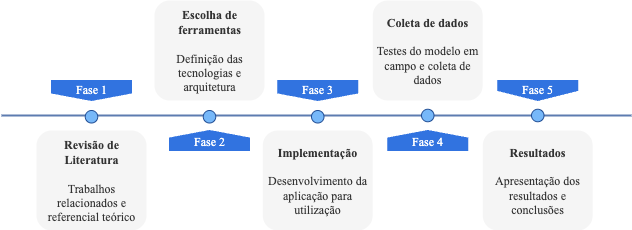
\includegraphics[width=\textwidth]{images/fases_pesquisa.png}
		\fonte{Elaborado pelo autor}
	\end{minipage}
\end{figure}
\FloatBarrier

\subsection{Proposta de Solução}

Conforme mencionado anteriormente, observa-se que o impacto da Inteligência Artificial no desenvolvimento de \textit{software} ainda é um tema em debate, sendo comum que as análises existentes se restrinjam a relatos de uso ou percepções subjetivas por parte dos desenvolvedores. Em muitos casos, a avaliação da influência da IA sobre fatores como produtividade e tempo de execução de tarefas ocorre de forma fragmentada, sem um método padronizado que permita mensurar de maneira objetiva os efeitos reais de tais ferramentas.

Dentro desse cenário, a proposta do estudo surge com a elaboração do um desafio técnico, disponibilizado através da plataforma \textit{web} desenvolvida especificamente para este fim. A ferramenta funcionou como um ambiente de avaliação controlado, no qual os participantes foram previamente organizados em dois grupos: um grupo com autorização para utilizar ferramentas de IA durante a resolução do desafio e outro grupo para realizar a atividade sem recorrer a tais recursos.

A proposta buscou, assim, criar condições equivalentes para ambos os grupos, garantindo que todos recebessem o mesmo enunciado do desafio, apresentado diretamente na plataforma. Para cada participante foi disponibilizado um \textit{link} único, correspondente ao grupo ao qual pertencia. A partir desse acesso, o desenvolvedor pôde visualizar as instruções, iniciar a tarefa e, ao concluir, submeter os arquivos com sua solução.

A plataforma também atuou como mecanismo de registro, armazenando automaticamente o tempo total gasto por cada participante, desde o momento em que deu início ao desafio até a finalização da entrega. Dessa forma, além da coleta da solução proposta, foi possível analisar métricas objetivas como tempo de conclusão, resolução dos problemas propostos (\textit{bugs}) e até mesmo, eventuais diferenças de abordagem entre os grupos.

\section{Modelo Proposto}

Esta seção tem como objetivo descrever brevemente a ferramenta desenvolvida e utilizada para a execução deste trabalho, incluindo sua arquitetura, funcionalidades e tecnologias utilizadas. O modelo proposto consiste em uma aplicação \textit{web} que centraliza as informações do desafio técnico, disponibilizando-o de forma prática e organizada para os desenvolvedores participantes do estudo.

A aplicação coleta o nome e o cargo atual do participante no mercado de trabalho. O nome é utilizado exclusivamente para exibir uma mensagem personalizada de boas-vindas. Funciona como um identificador simples durante a sessão, mantendo o usuário ativo no desafio, sem necessidade de cadastro, \textit{tokens} ou \textit{logins} complexos. Dessa forma, os nomes dos participantes não são utilizados na apresentação dos resultados do estudo, garantindo anonimato e simplicidade na utilização da ferramenta.

\subsection{Visão Geral}

A plataforma desenvolvida tem como objetivo oferecer um ambiente controlado, acessível e intuitivo para a realização de um desafio técnico. Sua concepção visa permitir a comparação entre dois grupos de participantes, um autorizado a utilizar ferramentas de IA Generativa e outro sem esse recurso, garantindo condições iguais de execução e coleta precisa de dados para análise posterior.

A aplicação dispõe de duas telas de cadastro semelhantes, diferenciadas apenas pelo tipo de participante. Uma é destinada aos desenvolvedores do grupo sem IA, e a outra aos do grupo com IA. Essa distinção é registrada internamente no banco de dados, identificando a qual grupo o participante pertence. A partir desse ponto, todo o fluxo de utilização da plataforma é idêntico para ambos os grupos, assegurando que todos recebam o mesmo desafio técnico, com os mesmos detalhes e informações.

Um aspecto essencial considerado durante o desenvolvimento foi o registro automático do tempo total de execução de cada participante. Esse recurso elimina a necessidade de solicitar uma estimativa manual de tempo após a conclusão, o que poderia gerar dados imprecisos e subjetivos. Assim, o sistema contabiliza precisamente o período compreendido entre o momento em que o participante inicia o desafio e o instante em que o finaliza.

Além disso, a plataforma foi projetada para proporcionar uma experiência simples e direta tanto para o acesso ao código-fonte do desafio quanto para o envio da solução desenvolvida. Ao término da atividade, o sistema disponibiliza um botão que direciona o participante ao formulário de \textit{feedback}, ajustado conforme o grupo ao qual pertence (sem ou com IA). Essa diferenciação se faz necessária, pois embora algumas perguntas sejam comuns entre os grupos, outras foram elaboradas especificamente para compreender a experiência de poder, ou não, utilizar ferramentas de IA generativa durante a execução do desafio.

\subsection{Arquitetura e Tecnologias}

A plataforma é dividida em três partes: a aplicação \textit{web}, uma \textit{API REST} e um banco de dados. A aplicação \textit{web} é responsável pelo formulário inicial (cadastro e identificação) dos desenvolvedores, exibição dos detalhes do desafio técnico e por todo o fluxo de etapas ao longo do experimento, como início do desafio, envio do arquivo com a solução por parte do desenvolvedor e finalização do desafio.

A \textit{API REST} é responsável por controlar toda a comunicação com o banco de dados do sistema, através das rotas configuradas que realizam operações como: registrar no banco de dados o tempo de ínicio do desenvolvedor (\textit{timestamp}) ao iniciar o desafio, registrar o tempo de término, armazenar o tempo total em milissegundos (ms) para a conclusão do desafio, armazenar o tipo do grupo do grupo do desenvolvedor (com ou sem IA), cargo do mesmo, realizar o download da pasta \textit{.zip} do código-fonte na máquina do participante, assim como realizar o \textit{upload} da solução do mesmo para o \textit{back-end}.

Sobre as tecnologias utilizadas, a aplicação \textit{web} foi desenvolvida utilizando \textit{React.js}\footnote{\textit{React.js}: \url{https://pt-br.reactjs.or}}. Esta biblioteca foi escolhida por ser bastante similar e utilizar \textit{JavaScript} como base, simplificando assim a construção da plataforma, até mesmo pela sua praticidade para a organização de páginas e componentes reutilizáveis entre elas, o que facilita muito a organização durante o desenvolvimento. Para otimizar a construção do \textit{front-end}, foi utilizado também a biblioteca \textit{Material UI}\footnote{\textit{Material UI}: \url{https://mui.com/material-ui/}}, uma biblioteca de componentes \textit{React}, \textit{open source}, que implementa o \textit{Material Design} do \textit{Google}.

Através das escolhas anteriores, acabou sendo determinante para que a \textit{API REST} fosse construída utilizando \textit{Express.js}\footnote{\textit{Express.js}: \url{https://expressjs.com/}}, sendo este um \textit{framework} minimalista e flexível para \textit{Node.js}\footnote{\textit{Node.js}: \url{https://nodejs.org/pt}}, que simplifica consideravelmente a criação de \textit{APIs}, fornecendo ferramentas para tarefas como roteamento e manipulação de requisições \textit{HTTP}. Além de prático com sua leveza e liberdade oferecida durante o processo de desenvolvimento, resultam em conseguir realizar a entrega de uma solução simples com mais precisão.

Por fim, a transferência de dados entre a aplicação web com a \textit{API} foi feita utilizando arquivos \textit{JSON}, recebendo-os e manipulando-os. Para o banco de dados, foi utilizado \textit{PostgreSQL}\footnote{\textit{PostgreSQL}: \url{https://www.postgresql.org/}}, por ser um banco de dados relacional de objeto e \textit{open source}, conhecido por sua robustez, confiabildade, extensibilidade e até mesmo, fácil manuseio e implementação. Ele suporta tanto dados relacionais (\textit{SQL}) quanto não relacionais (\textit{JSON}), compatibilidade com padrões \textit{SQL}, e funcionalidades avançadas como chaves estrangeiras, gatilhos e recuperação pontual. Por ser \textit{open soruce}, o \textit{PostgreSQL} é igualmente gratuito. Para a estrutura das tabelas e seus dados, foi seguido o modelo de dados relacionais (\textit{SQL}), afinal, foram necessárias somente três tabelas para o banco de dados, sendo elas:

\begin{itemize}[leftmargin=1cm, itemsep=0.1em, topsep=0.1em]
    \item \textit{Developer}, responsável por armazenar as informações do administrador e dos participantes;
    \item \textit{Challenge}, responsável por armazenar os dados de início, término e tempo total da conclusão do desafio de cada participante;
    \item \textit{DeveloperChallenge}, responsável por armazenar os dados referentes ao arquivo de solução do desenvolvedor.
\end{itemize}

O diagrama ER do banco de dados está disponível no Apêndice A. Sobre o \textit{deploy} de todas as camadas da plataforma, a aplicação \textit{web} foi hospedada na plataforma \textit{Vercel}\footnote{\textit{Vercel}: \url{ https://vercel.com/}}, que possui planos gratuitos e também pela  praticidade de sua integração ao repositório no \textit{GitHub}\footnote{\textit{GitHub}: \url{https://github.com/}}, que facilita no processo de \textit{deploys} automáticos conforme novos \textit{commits} vão sendo feitos ao repositório remoto.

Por fim, a \textit{API} e o banco de dados \textit{PostgreSQL} foram hospedados na plataforma \textit{Railway}\footnote{\textit{Railway}: \url{https://railway.com/}}, por possuir planos com créditos limitados para consumo/uso por alguns dias ou até o término dos créditos. Sua versatilidade para igualmente integrar ao repositório no \textit{GitHub}, também trouxe praticidade para que o \textit{deploy} da \textit{API} fosse realizado sem muitas complicações a cada novo \textit{commit}. Para o banco de dados, foi exportado somente o arquivo \texttt{.dump} do ambiente local de desenvolviemnto e importado para o \textit{Railway}.

As ferramentas utilizadas no processo de desenvolvimento foram o \textit{Visual Studio Code}\footnote{\textit{Visual Studio Code}: \url{https://code.visualstudio.com/}} (\textit{VS Code}), editor de código-fonte popularmente conhecido, especialmente para o desenvolvimento de aplicações \textit{web} e praticipade para o uso do \textit{terminal} dentro do \textit{VS Code}. Outra ferramenta utilizada para os testes das rotas da \textit{API} a medida em que iam sendo criadas, antes de serem integradas ao \textit{front-end}, foi a ferramenta \textit{Postman}\footnote{\textit{Postman}: \url{https://www.postman.com/}}, por facilitar a criação, testes e documentação de \textit{APIs}, permitindo o envio de requisições \textit{HTTP}/\textit{HTTPS}. Com sua interface intuitiva, se tornou prático ir fazendo o acompanhamento das requisições que eram feitas e a armazenagem dos dados no banco.

Um breve diagrama da arquitetura do modelo é ilustrado na Figura \ref{fig:arquitetura}.

\begin{figure}[ht]
    \caption{Arquitetura do modelo}
    \label{fig:arquitetura}
    \centering
    \footnotesize
    \begin{minipage}{.9\textwidth}
        \centering
        \fbox{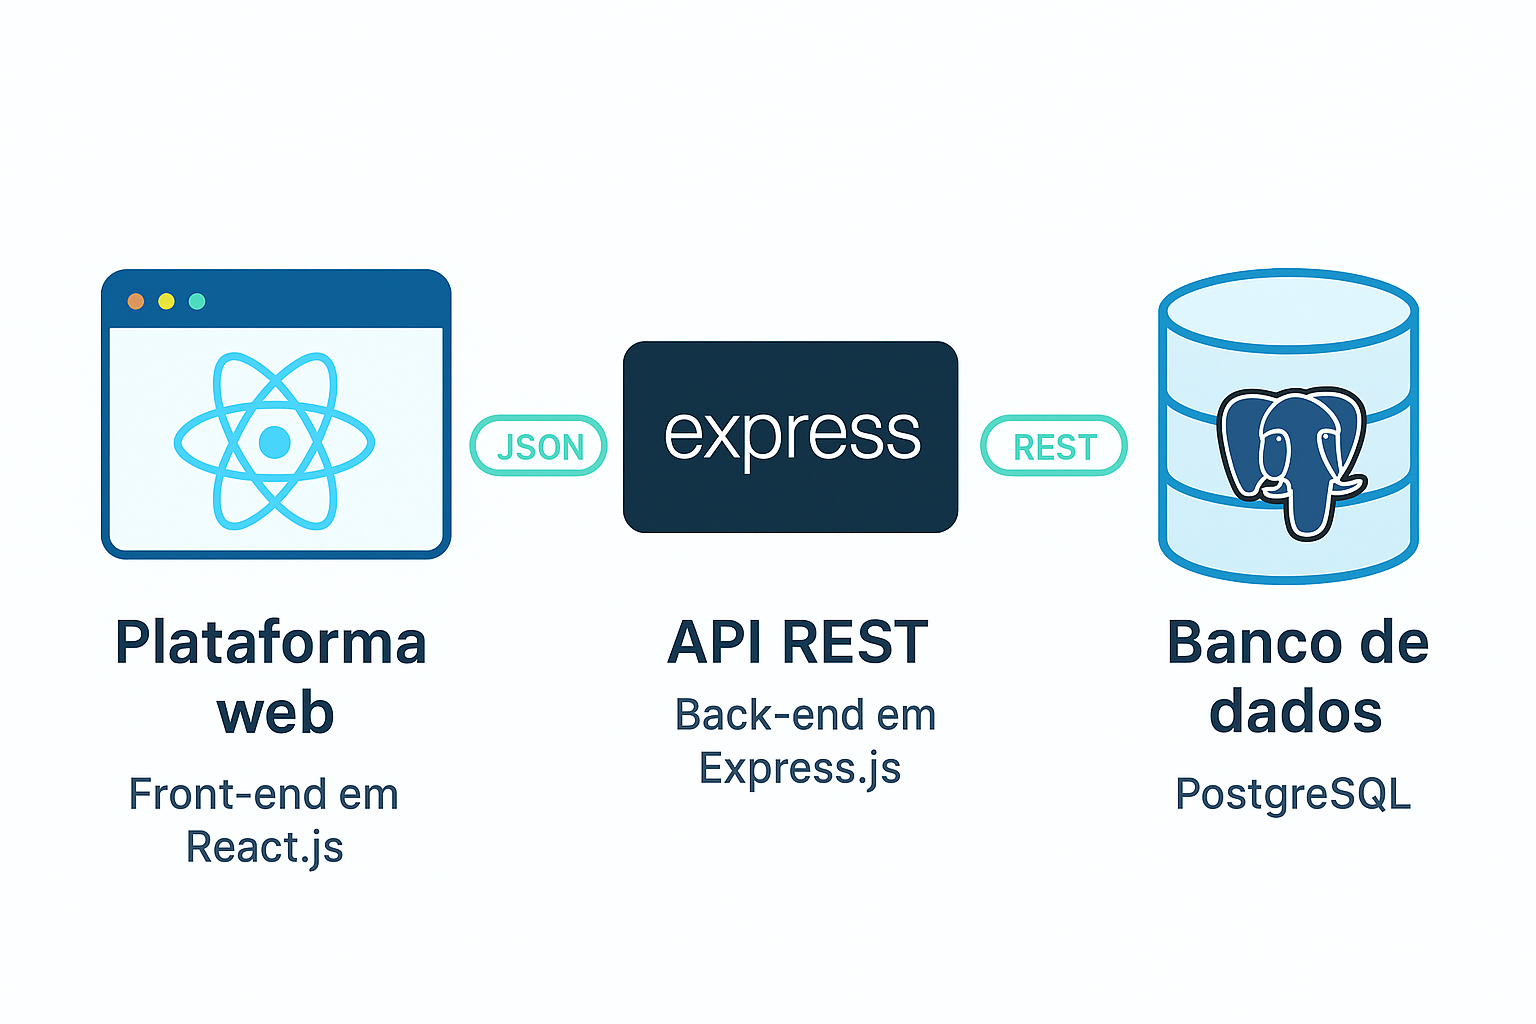
\includegraphics[width=0.50\textwidth]{images/arquitetura.png}}
        \fonte{Elaborado pelo autor}
    \end{minipage}
\end{figure}
\FloatBarrier

\subsection{Funcionalidades}

A seguir serão apresentadas as principais funcionalidades da plataforma proposta para o desenvolvimento deste modelo, detalhando cada um delas. Nesta seção estão as telas dos fluxos  de uso e etapas dentro da plataforma. As demais telas estão disponíveis no Apêndice B.

\subsection{Formulário Inicial}

Ao acessar a plataforma \textit{web} através do \textit{link} fornecido juntamente com as instruções iniciais via \textit{WhatsApp} para cada participante, o desenvolvedor necessita preencher um breve formulário informando seu "Nome e Sobrenome" (que é somente de uso interno na plataforma), seu "Cargo atual" e então pressionar o botão "Registrar". Os campos "Nome e Sobrenome" e "Cargo atual" são obrigatórios para o participante poder avançar. Na Figura \ref{fig:cadastro_sem_ia} está a tela de registro do participante do grupo sem IA e na Figura \ref{fig:cadastro_com_ia} está a tela de registro do participante do grupo com IA, respectivamente.

\begin{figure}[ht]
    \caption{Cadastro do participante do grupo sem IA}
    \label{fig:cadastro_sem_ia}
    \centering
    \footnotesize
    \begin{minipage}{.9\textwidth}
        \centering
        \fbox{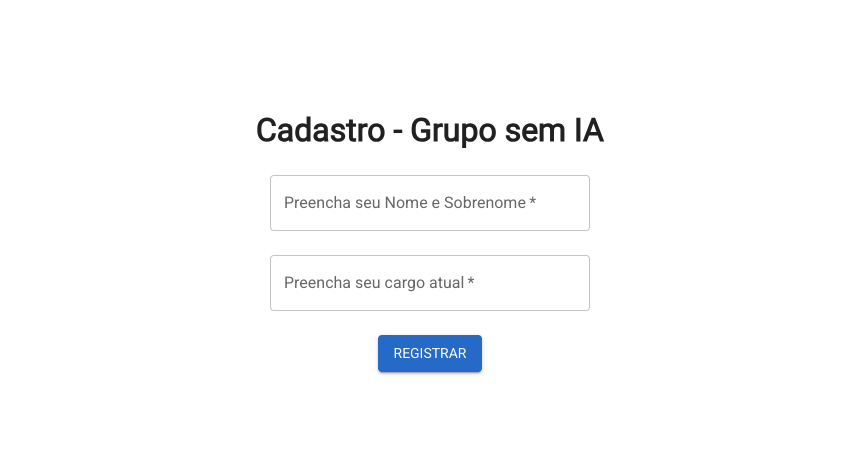
\includegraphics[width=0.95\textwidth]{images/cadastro_sem_ia.png}}
        \fonte{Elaborado pelo autor}
    \end{minipage}
\end{figure}
\FloatBarrier

\begin{figure}[ht]
    \caption{Cadastro do participante do grupo com IA}
    \label{fig:cadastro_com_ia}
    \centering
    \footnotesize
    \begin{minipage}{.9\textwidth}
        \centering
        \fbox{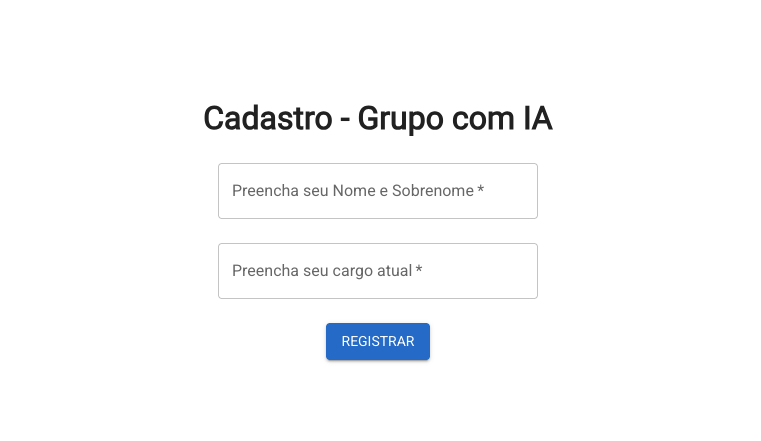
\includegraphics[width=0.95\textwidth]{images/cadastro_com_ia.png}}
        \fonte{Elaborado pelo autor}
    \end{minipage}
\end{figure}
\FloatBarrier

\subsection{Tela Inicial e Informações do Desafio}

Após o preenchimento do formulário inicial, o participante é direcionado para a primeira tela da plataforma, que neste caso é a tela do desafio técnico propriamente. Porém, nesta tela, antes de exibir os detalhes do desafio, é exibido mais algumas informações que reforçam a necessidade de atenção e dedicação do participante antes de dar início ao teste. 

Estando de acordo, o participante clica no botão "De acordo" e na mesma tela é renderizada todos os detalhes e imagens de cenários de exemplo, descrevendo o desafio técnico que o desenvolvedor irá solucionar. A tela inicial e as informações do desafio encontram-se na Figura \ref{fig:tela_inicial} e Figura \ref{fig:informacoes_desafio}, respectivamente.

\begin{figure}[ht]
    \caption{Tela inicial}
    \label{fig:tela_inicial}
    \centering
    \footnotesize
    \begin{minipage}{.9\textwidth}
        \centering
        \fbox{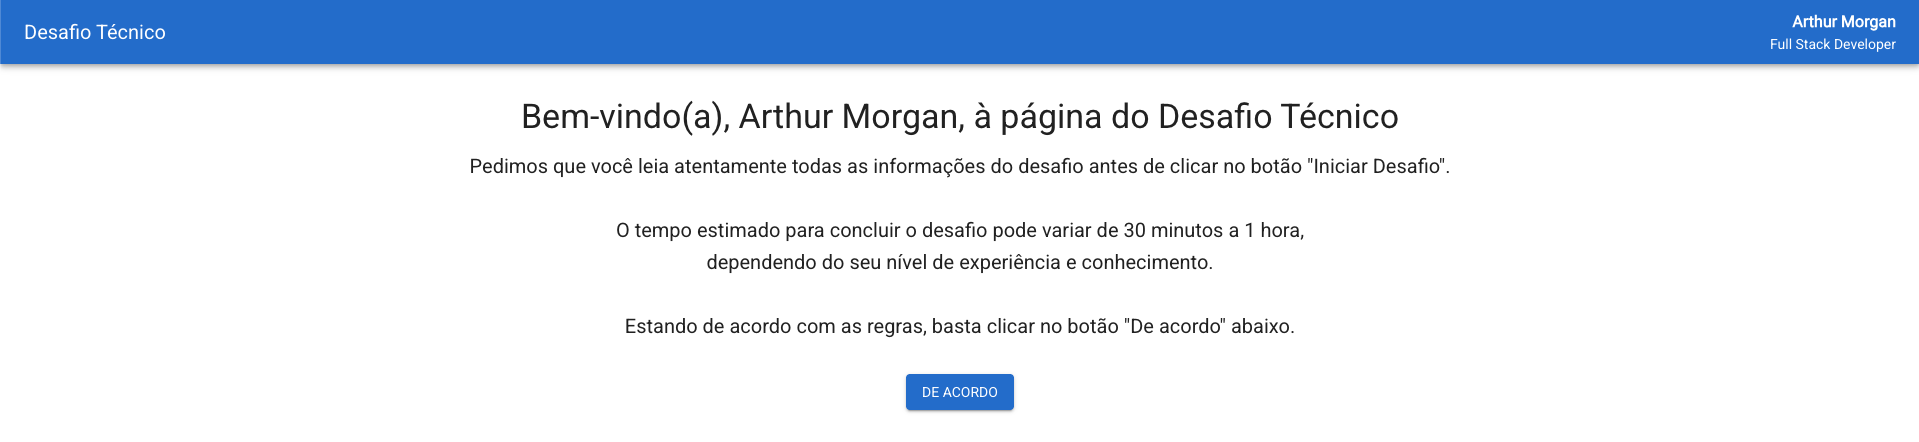
\includegraphics[width=0.95\textwidth]{images/tela_inicial.png}}
        \fonte{Elaborado pelo autor}
    \end{minipage}
\end{figure}
\FloatBarrier

\begin{figure}[ht]
    \caption{Informações do desafio}
    \label{fig:informacoes_desafio}
    \centering
    \footnotesize
    \begin{minipage}{.9\textwidth}
        \centering
        \fbox{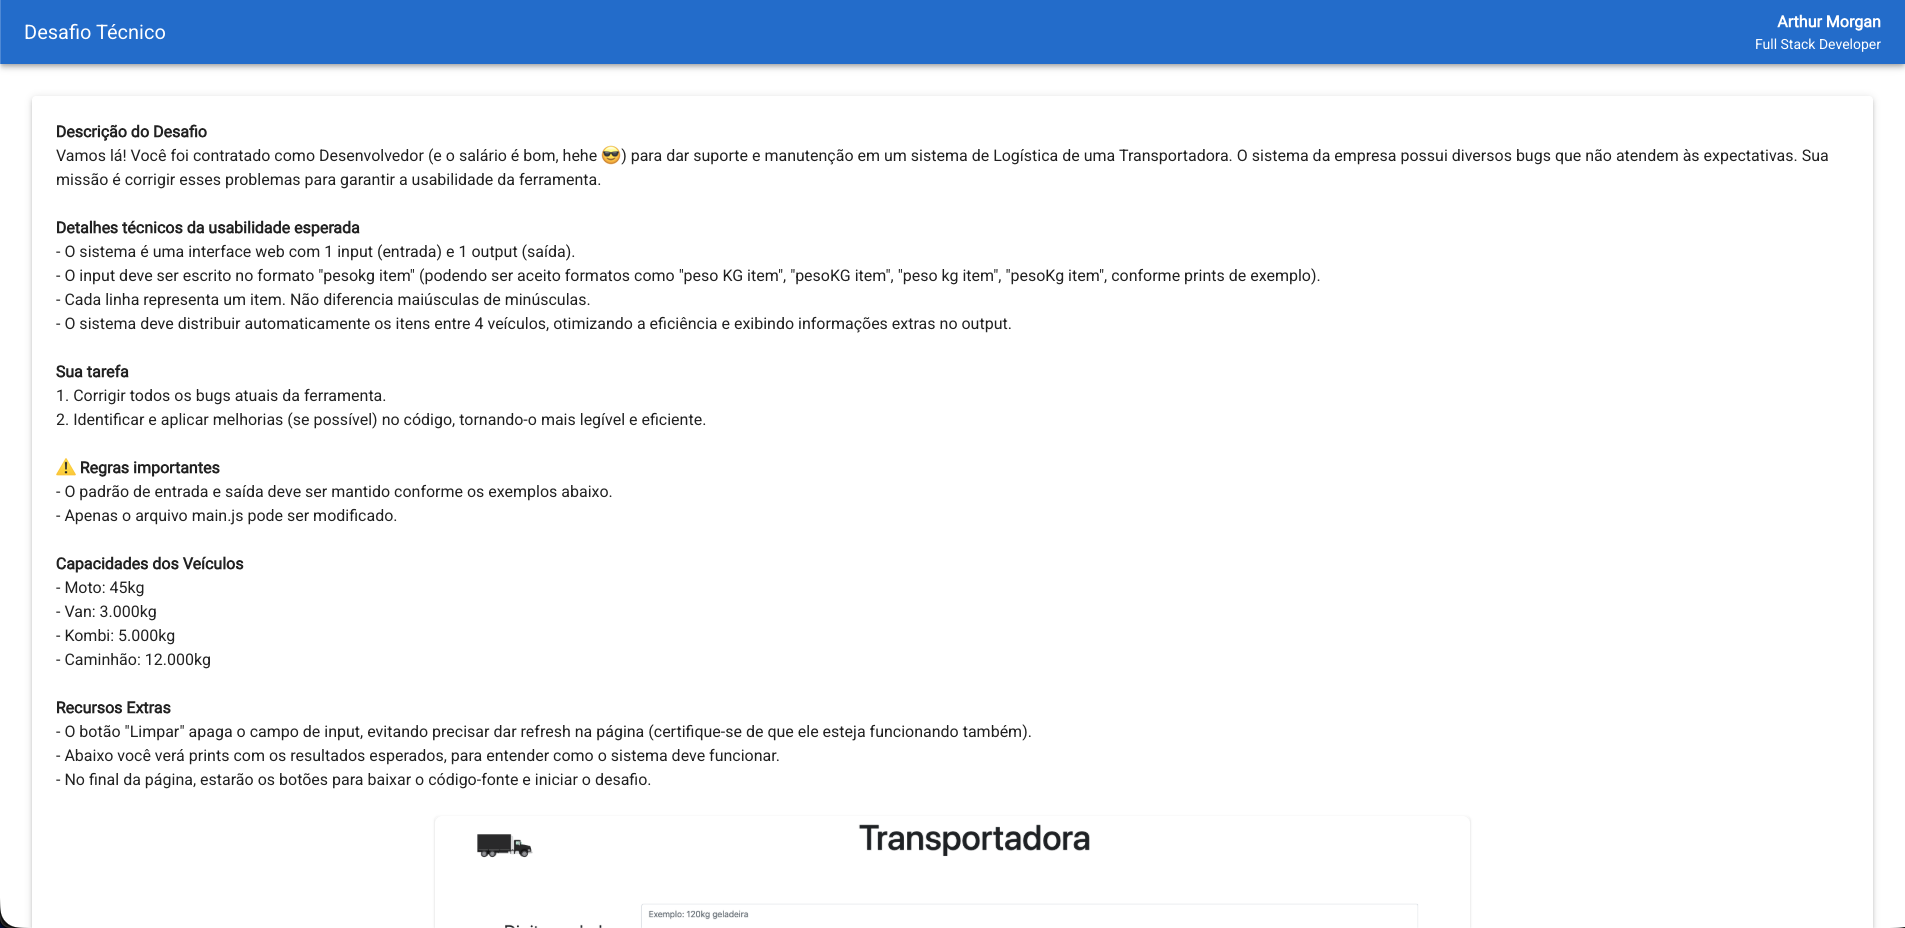
\includegraphics[width=0.95\textwidth]{images/informacoes_desafio.png}}
        \fonte{Elaborado pelo autor}
    \end{minipage}
\end{figure}
\FloatBarrier

Ao descer um pouco a tela, o desenvolvedor encontra as imagens de cenários de exemplo que ilustram o objetivo final das funcionalidades que a solução precisa atender para concluir o desafio de modo satisfatório, como exemplo da Figura \ref{fig:exemplos_desafio}.

\begin{figure}[ht]
    \caption{Cenário de exemplo}
    \label{fig:exemplos_desafio}
    \centering
    \footnotesize
    \begin{minipage}{.9\textwidth}
        \centering
        \fbox{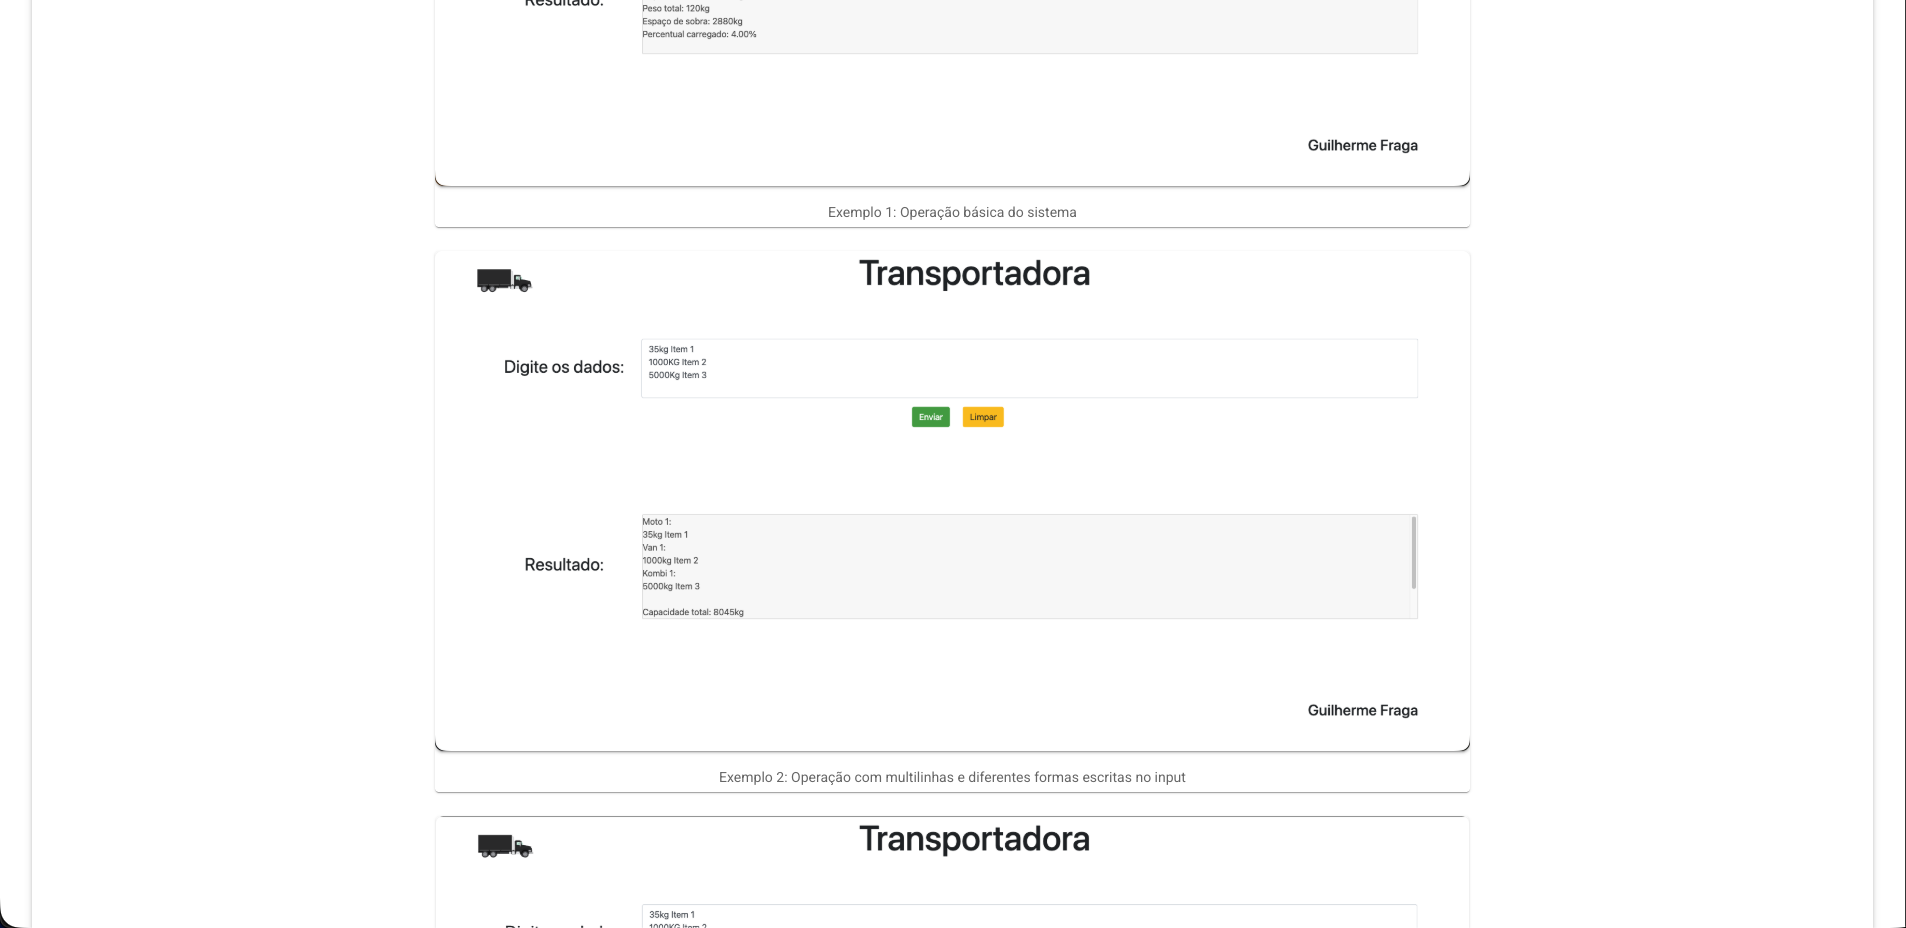
\includegraphics[width=0.95\textwidth]{images/exemplos_desafio.png}}
        \fonte{Elaborado pelo autor}
    \end{minipage}
\end{figure}
\FloatBarrier

Ao final da tela, conforme a Figura \ref{fig:baixar_iniciar_desafio}, está o botão para realizar o \textit{download} do código-fonte do desafio técnico e logo abaixo, o botão para iniciar o desafio, que só é habilitado após o participante acionar o anterior, ou seja, realizar o \textit{download}. Nesta parte também foi colocado mais um aviso reforçando a importância do participante preparar seu ambiente de desenvolvimento antes de clicar em "iniciar desafio", pois ao acionar este botão, uma rota da \textit{API} é chamada que armazena no banco de dados o horário de início (\textit{timestamp}) do desenvolvedor, registrando assim o momento exato em que o participante iniciou a atividade.

\begin{figure}[ht]
    \caption{Baixar e iniciar desafio}
    \label{fig:baixar_iniciar_desafio}
    \centering
    \footnotesize
    \begin{minipage}{.9\textwidth}
        \centering
        \fbox{
\includegraphics[width=0.95\textwidth]{images/baixar_iniciar_desafio.png}}
        \fonte{Elaborado pelo autor}
    \end{minipage}
\end{figure}
\FloatBarrier

\subsection{Desafio Técnico}

Para projetar o desafio técnico proposto dentro da plataforma, imaginou-se um cenário fictício, onde para isso foi reaproveitado um projeto particular utilizado anteriormente pelo pesquisador apenas para fins de estudo pessoal. Este projeto consiste em um sistema simples de logística de uma transportadora, onde, conforme mencionado anteriormente, trata-se de uma interface \textit{web} básica, que permite a entrada de um \textit{input} e retorna um \textit{output}.

Sendo assim, os dados de \textit{input} que são utilizados, nada mais são do que itens, no formato "pesokg item" (podendo ser aceito formatos como "peso KG item", "peso kg item" e etc.), que representam itens em que o sistema da transportadora deverá alocar automaticamente em cada tipo de veículo de acordo com a capacidade do mesmo e de acordo com o peso do item, otimizando a eficiência e exibindo os detalhes necessários de acordo com o \textit{output} esperado pelo sistema.

No campo de \textit{input} do sistema, cada linha representa um item, não diferenciando letras maiúsculas de minúsculas. Neste sistema, foram alocados quatro tipos de veículos com suas respectivas capacidades. Numa simulação, mais de um mesmo tipo de veículo poderia ser utilizado se, de acordo com os pesos dos itens, encaixassem neste mesmo tipo de veículo. Como por exemplo: 2 itens de 45kg, o veículo do tipo "moto" possui capacidade de 45kg, ou seja, seria alocado "duas motos" para carregarem estas cargas.

Para o desafio técnico, foi fornecido todo o código-fonte do sistema, incluindo arquivos como \texttt{index.html}, \texttt{style.css}, que compõem a interface \textit{web} do desafio. Entretanto, como regra do desafio, foi exigido para os participantes que só realizassem as alterações no arquivo \texttt{main.js}, visto que este contém toda a lógica de negócio para as funcionalidades exigidas no sistema de logística. Assim, seria mais prático para os desenvolvedores utilizarem da interface \textit{web} já pronta, sem a necessidade de ajustes, para a realização de testes manuais à medida que iriam realizando as correções necessárias para atingir os objetivos.

Isto dito, tendo como referência o código-fonte base (disponível completo no Apêndice G), foram sendo adicionados diversos \textit{bugs} propositais no arquivo \texttt{main.js}, ou seja, sendo quebrado o código em diversas partes, para que os participantes do experimento solucionassem os mesmos. Estes \textit{bugs} foram organizados em uma lista para controle e análises posteriores, após a conclusão e envio das soluções dos desenvolvedores, que encontra-se no Apêndice H. O arquivo \texttt{main.js} fornecido para os desenvolvedores com os \textit{bugs} encontra-se disponível no Apêndice G.

\subsection{Tela de \textit{Upload}}

Após o participante clicar no botão "Iniciar Desafio", o mesmo é direcionado para a tela de \textit{upload}. Nesta tela, as informações referentes ao desafio permanecem sem alterações, para que fosse possível ao participante consultar a medida que fosse solucionando os \textit{bugs}. O diferencial desta tela se dá pelo título no topo, conforme a Figura \ref{fig:tela_upload}, indicando ao participante que ao término da sua solução, o mesmo deve descer até o final da página para realizar o envio do seu arquivo através dos botões indicados. 

\begin{figure}[ht]
    \caption{Tela de \textit{Upload}}
    \label{fig:tela_upload}
    \centering
    \footnotesize
    \begin{minipage}{.9\textwidth}
        \centering
        \fbox{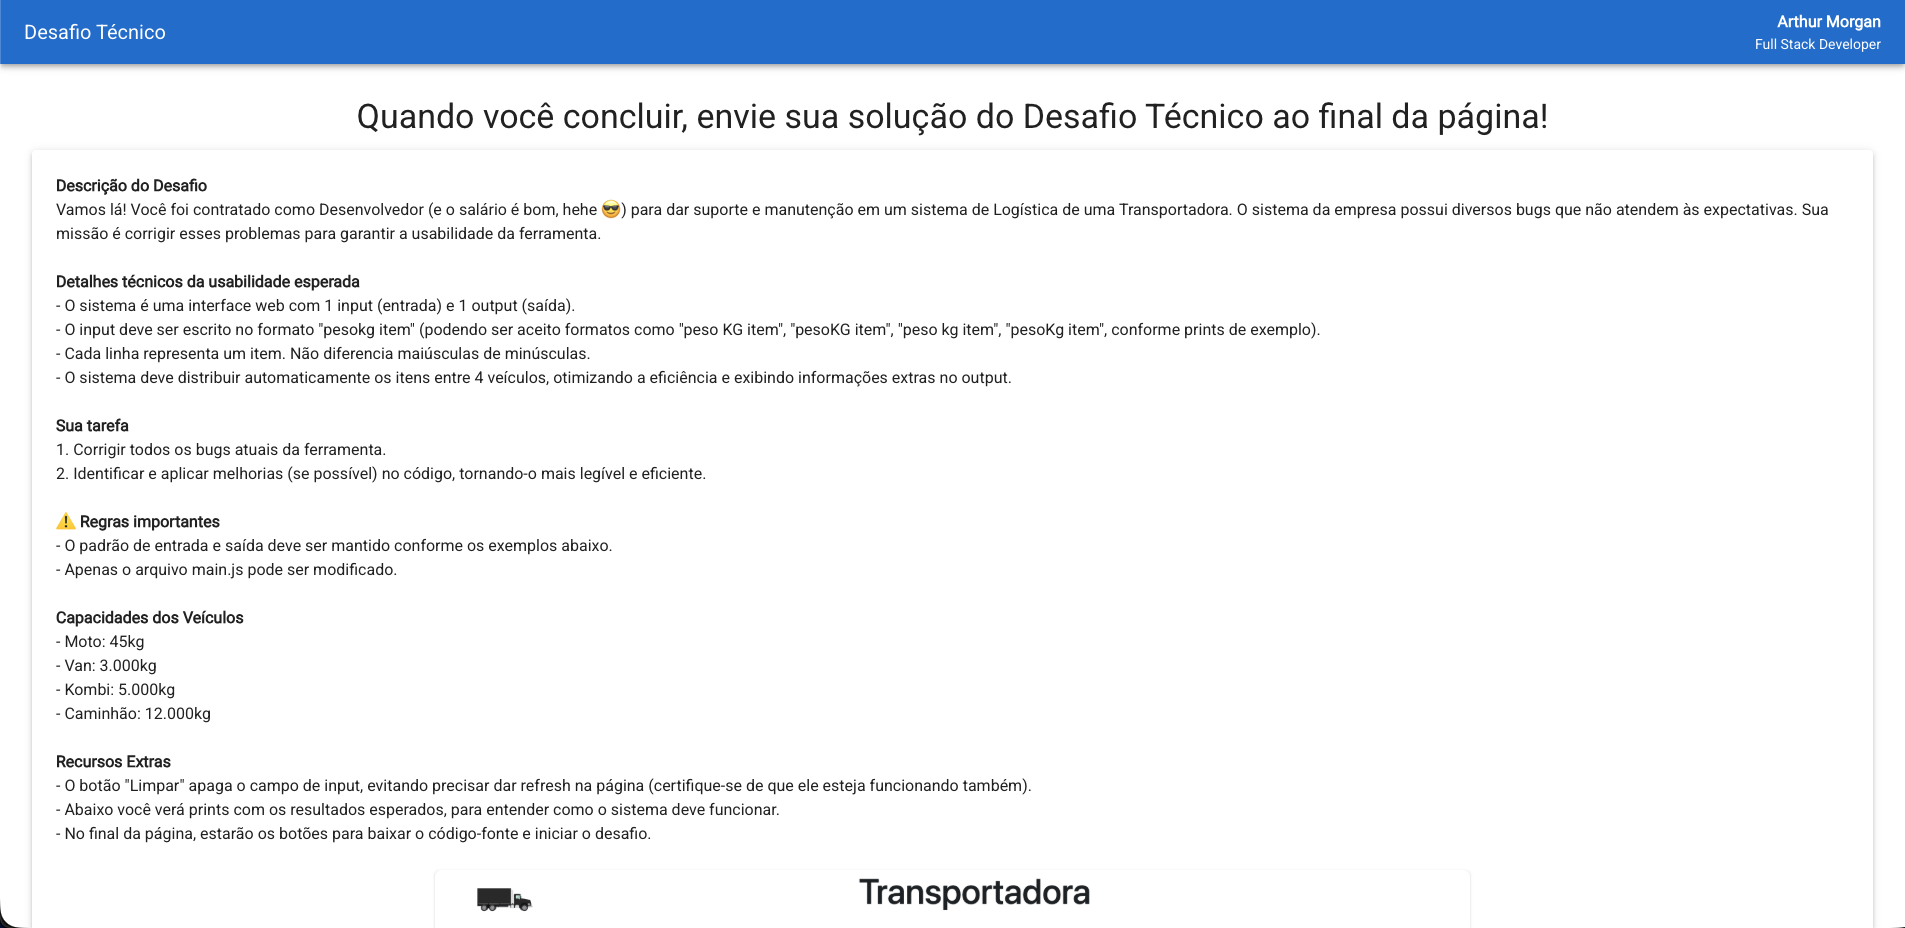
\includegraphics[width=0.95\textwidth]{images/tela_upload.png}}
        \fonte{Elaborado pelo autor}
    \end{minipage}
\end{figure}
\FloatBarrier

No final da página, encontram-se os botões para o participante selecionar seu arquivo e finalizar o desafio. O segundo botão só é habilitado após um arquivo ser selecionado. A plataforma ainda permite após escolher um arquivo, editar para selecionar outro, caso o primeiro tenha sido escolhido erroneamente ou caso o participante tenha feito alguma alteração antes de, de fato, finalizar o desafio.

Para fins de tornar mais prático a experiência do participante, foi limitado para que a plataforma aceitasse apenas arquivos \textit{.zip}, pensando no cenário de que, após a conclusão por parte do desenvolvedor, o mesmo só precisaria compactar a pasta completa da sua solução e realizar o envio. Uma vez que o arquivo é selecionado, a aplicação o armazena em uma pasta temporária (\textit{tmp}) no \textit{back-end} e, após clicar no botão "Finalizar Desafio", a rota da \textit{API} responsável por encerrar o desafio é chamada, onde então é armazenado no banco de dados o \textit{timestamp} de conclusão do desenvolvedor e feito o cálculo da diferença entre o \textit{timestamp} de conclusão e de início, para igualmente armazenar no banco de dados o tempo total, em milissegundos (ms) da duração para o participante concluir o desafio. Após isso, o arquivo é movido da pasta \textit{tmp} para a pasta \textit{uploads} no \textit{back-end}. Na Figura \ref{fig:selecionar_arquivo_finalizar_desafio} encontra-se os botões mencionados acima.

\begin{figure}[ht]
    \caption{Selecionar arquivo e finalizar desafio}
    \label{fig:selecionar_arquivo_finalizar_desafio}
    \centering
    \footnotesize
    \begin{minipage}{.9\textwidth}
        \centering
        \fbox{
\includegraphics[width=0.95\textwidth]{images/selecionar_arquivo_finalizar_desafio.png}}
        \fonte{Elaborado pelo autor}
    \end{minipage}
\end{figure}
\FloatBarrier

Após o desafio finalizado, o participante é direcionado para uma tela final de agradecimento, com um botão para direcioná-lo ao preenchiemnto do formulário de \textit{feedback} do experimento através da ferramenta \textit{Google Forms}\footnote{\textit{Google Forms}: \url{https://workspace.google.com/intl/pt-BR/products/forms/}}, conforme a Figura \ref{fig:tela_final_formulario} abaixo.

\begin{figure}[ht]
    \caption{Tela final e formulário}
    \label{fig:tela_final_formulario}
    \centering
    \footnotesize
    \begin{minipage}{.9\textwidth}
        \centering
        \fbox{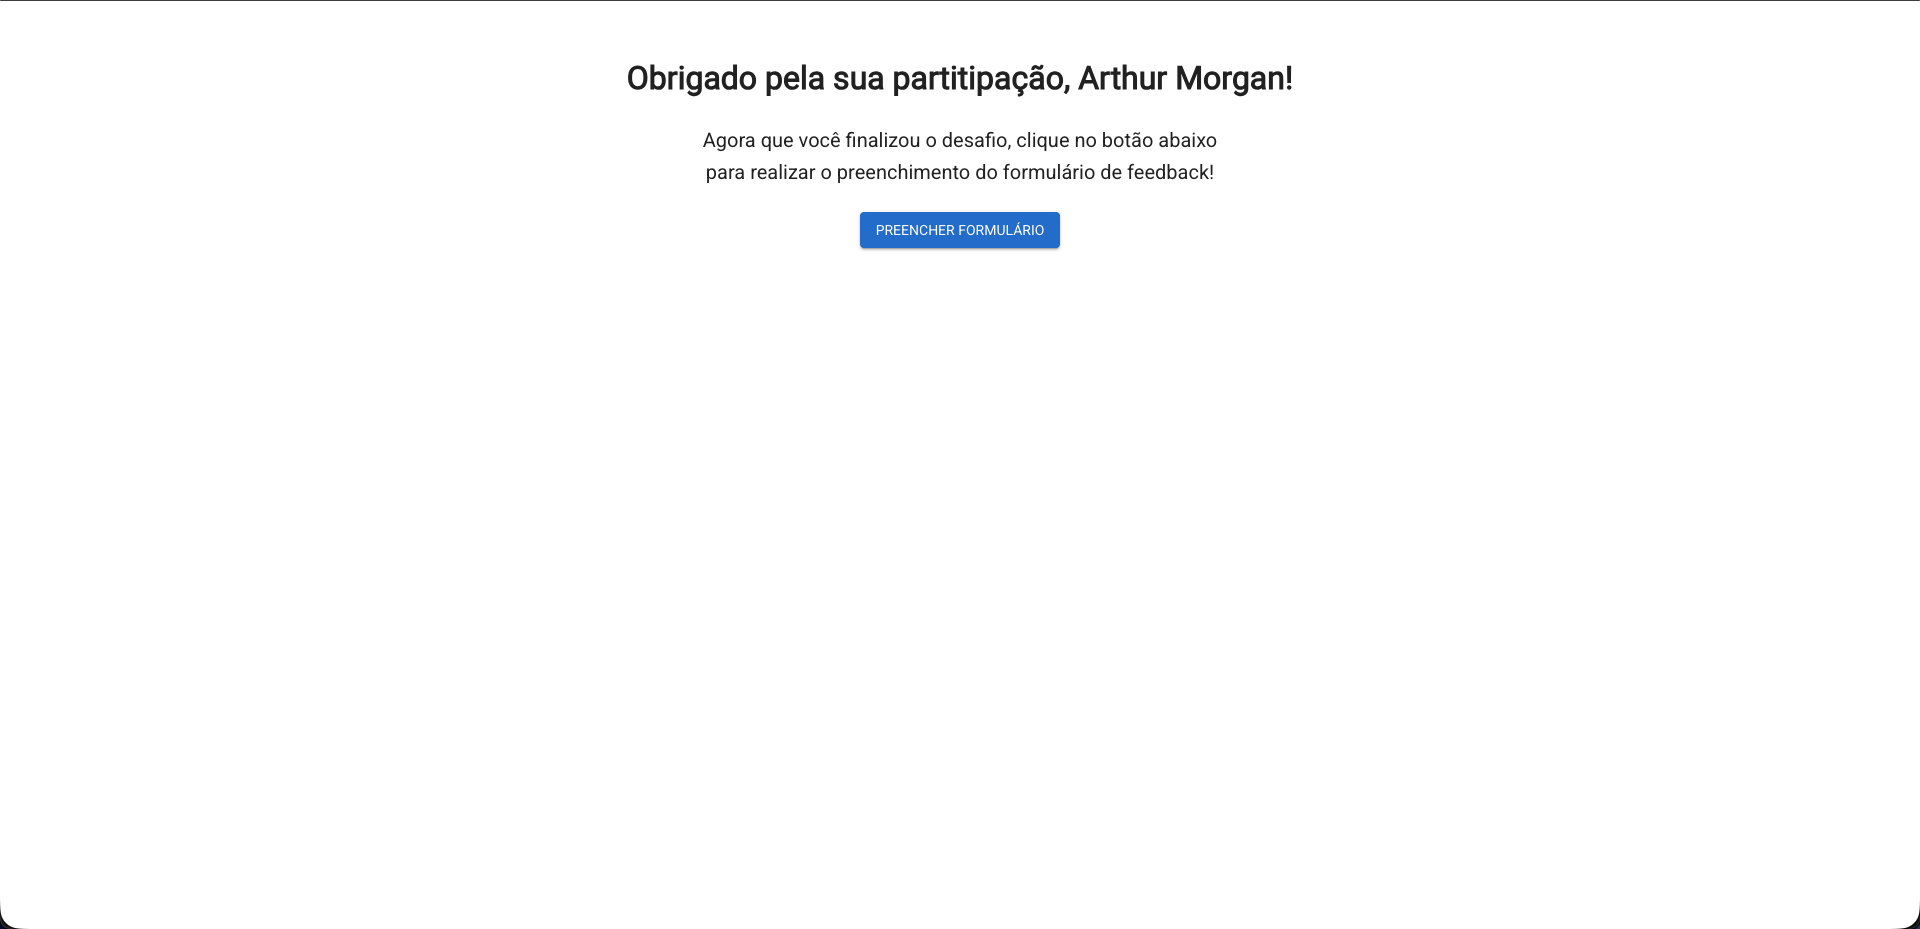
\includegraphics[width=0.95\textwidth]{images/tela_final_formulario.png}}
        \fonte{Elaborado pelo autor}
    \end{minipage}
\end{figure}
\FloatBarrier

\subsection{Painel de Administrador}

O acompanhamento das soluções dos desenvolvedores foram realizadas através de um painel de uso exclusivo do administrador do experimento. Este painel foi projetado com o objetivo de centralizar as informações principais dos participantes, agrupando-os em dados gerais e em seus grupos alocados (sem IA e com IA). O acesso deste painel é feito através de um \textit{link}\footnote{\textit{Link} para o Painel de Administrador: \url{https://ai-use-productivity.vercel.app/admin}}, que funciona como um "login" simples, apenas informando o nome do administrador, que aciona uma rota da API para validar se este nome informado está registrado no banco de dados como administrador. Esta tela encontra-se na Figura \ref{fig:painel_admin}.

\begin{figure}[ht]
    \caption{Acesso ao Painel de Administrador}
    \label{fig:painel_admin}
    \centering
    \footnotesize
    \begin{minipage}{.9\textwidth}
        \centering
        \fbox{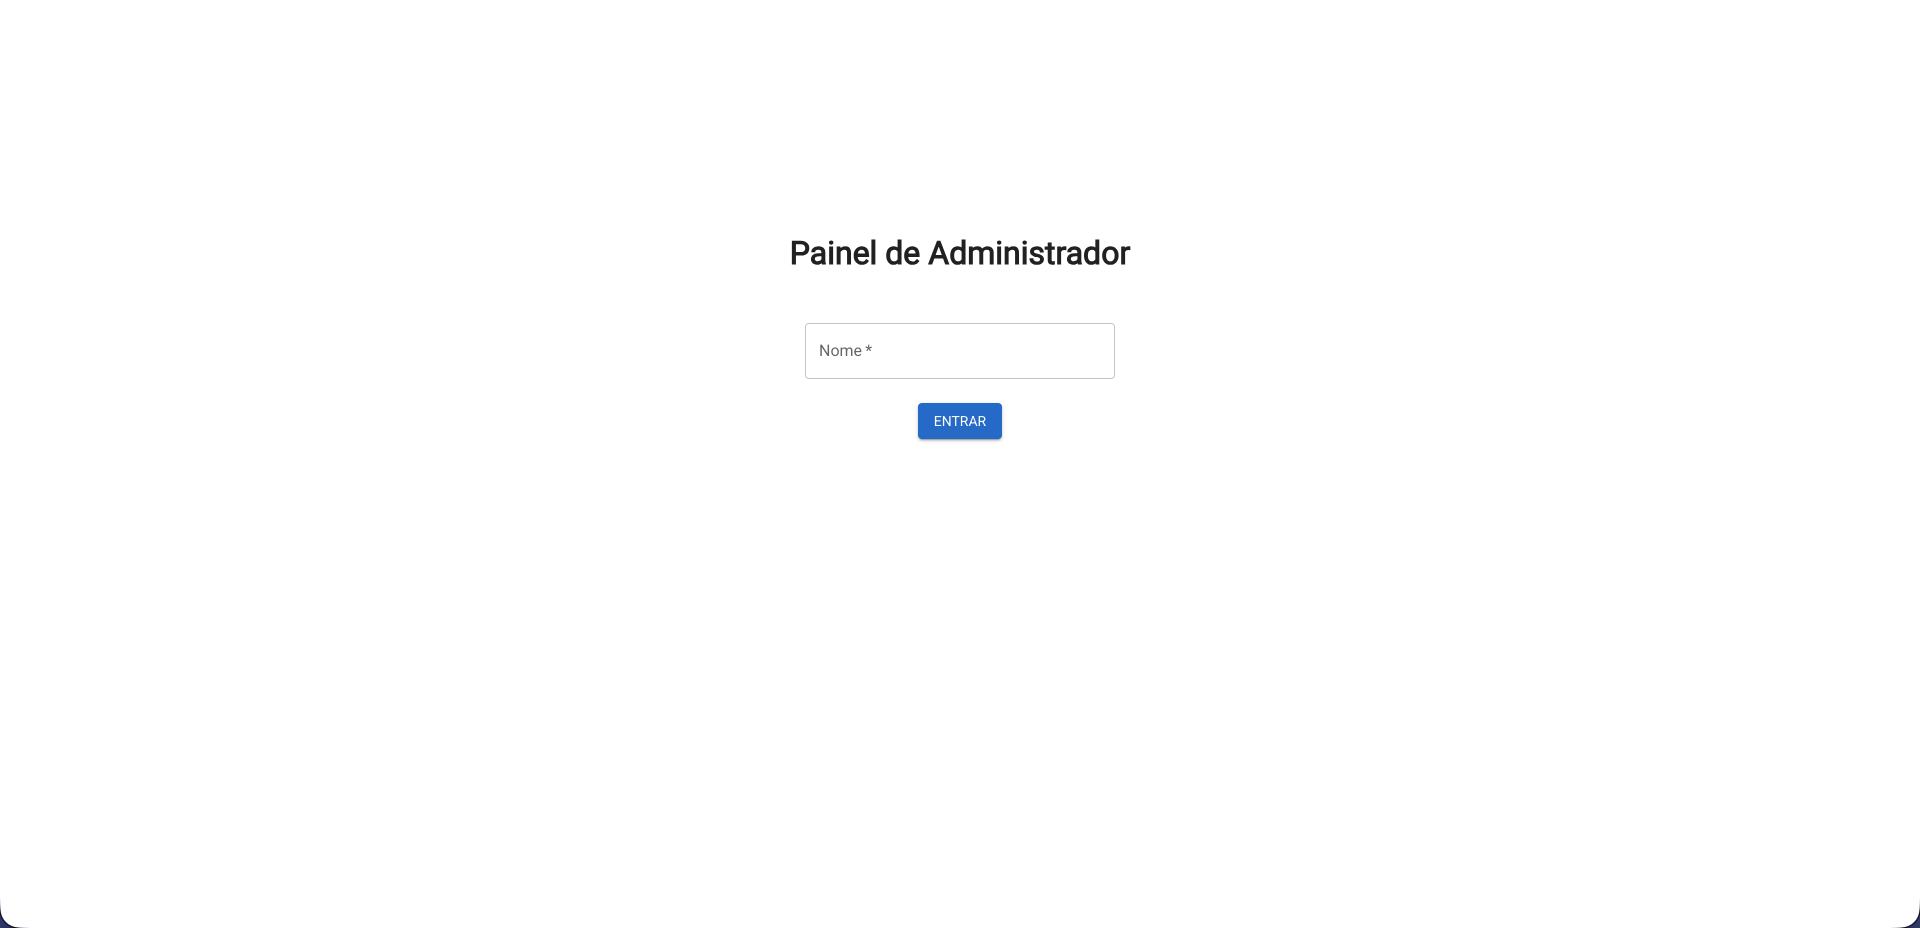
\includegraphics[width=0.95\textwidth]{images/painel_admin.png}}
        \fonte{Elaborado pelo autor}
    \end{minipage}
\end{figure}
\FloatBarrier

Acessando então como administrador, direciona-se para a tela de painel central, onde exibe informações gerais como o total de participantes do experimento, quantos pertencem ao grupo com IA, quantos pertencem ao grupo sem IA, a quantidade de arquivos enviados (soluções dos desenvolvedores) e o tempo médio geral de todos os participantes. A Figura \ref{fig:painel_central_admin} demonstra esta tela.

\begin{figure}[ht]
    \caption{Painel Central}
    \label{fig:painel_central_admin}
    \centering
    \footnotesize
    \begin{minipage}{.9\textwidth}
        \centering
        \fbox{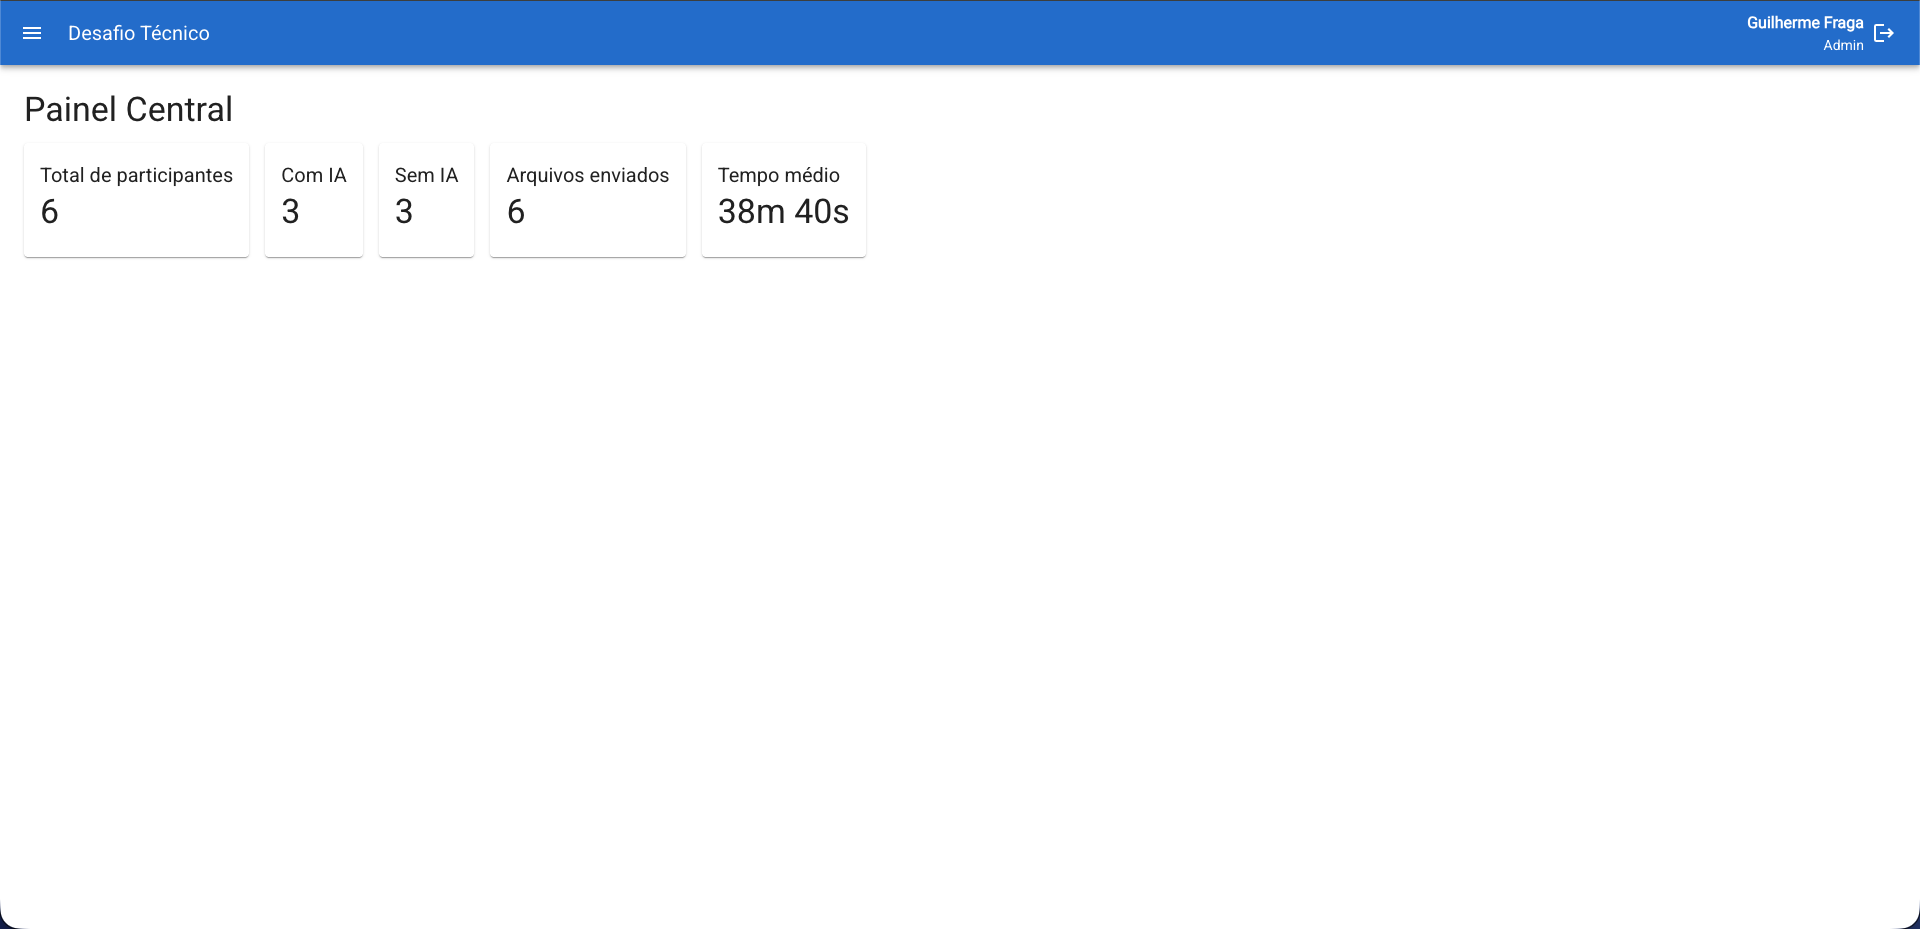
\includegraphics[width=0.95\textwidth]{images/painel_central_admin.png}}
        \fonte{Elaborado pelo autor}
    \end{minipage}
\end{figure}
\FloatBarrier

Através da barra de menu lateral à esquerda, tem-se a opção de "Resultados", que igualmente, exibe todos os resultados, individuais, de cada um dos participantes, em formatos de "\textit{cards}". Para cada participante é exibido o seu cargo, o tempo total que o mesmo levou para concluir o desafio, o grupo ao qual pertencia e o nome do seu arquivo enviado. Para facilitar no momento de identificação dos arquivos, foi realizada uma lógica para que, no momento em que o participante fizesse o \textit{upload} da sua solução, o arquivo fosse salvo no \textit{backend} seguindo uma lógica de ``\textit{id-Nome\_Sobrenome-nome\_do\_arquivo\_do\_participante.zip}''. Ao lado do nome de cada arquivo de cada participante, há o botão "Baixar", para realizar o \textit{download} da solução do desenvolvedor para as análises posteriores. O exemplo desta tela encontra-se na Figura \ref{fig:resultados_gerais_admin}. Com o intuito de manter o anonimato dos participantes do experimento, as imagens dos resultados do painel de adminsitrador foram editadas para ocultar os nomes dos desenvolvedores.

\begin{figure}[ht]
    \caption{Resultados}
    \label{fig:resultados_gerais_admin}
    \centering
    \footnotesize
    \begin{minipage}{.9\textwidth}
        \centering
        \fbox{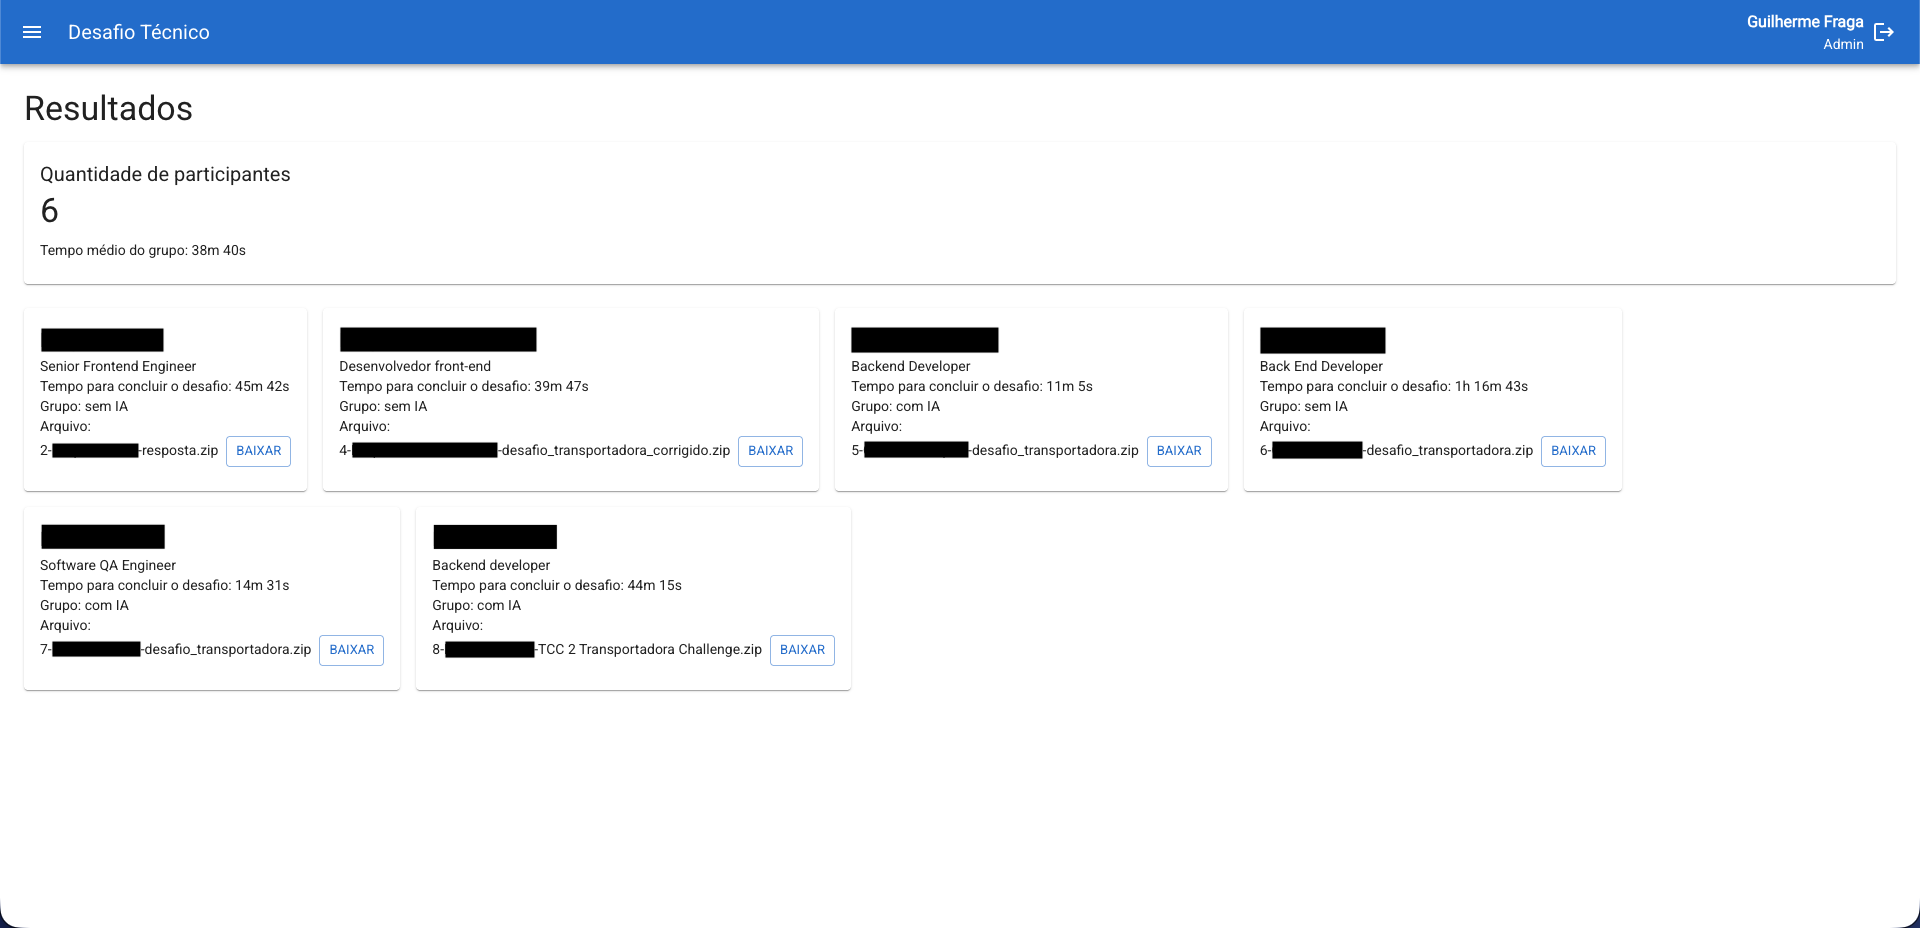
\includegraphics[width=0.95\textwidth]{images/resultados_gerais_admin.png}}
        \fonte{Elaborado pelo autor}
    \end{minipage}
\end{figure}
\FloatBarrier

As outras duas opções dos menus na barra lateral são para separar os resultados nos dois grupos, através da tela "Resultados Desenvolvedores sem IA" e "Resultados Desenvolvedores com IA". Os exemplos destas telas com os resultados do grupo sem IA e com IA, podem ser conferidos através das Figuras \ref{fig:resultados_sem_ia_admin} e \ref{fig:resultados_com_ia_admin}, respectivamente.

\begin{figure}[ht]
    \caption{Resultados Desenvolvedores sem IA}
    \label{fig:resultados_sem_ia_admin}
    \centering
    \footnotesize
    \begin{minipage}{.9\textwidth}
        \centering
        \fbox{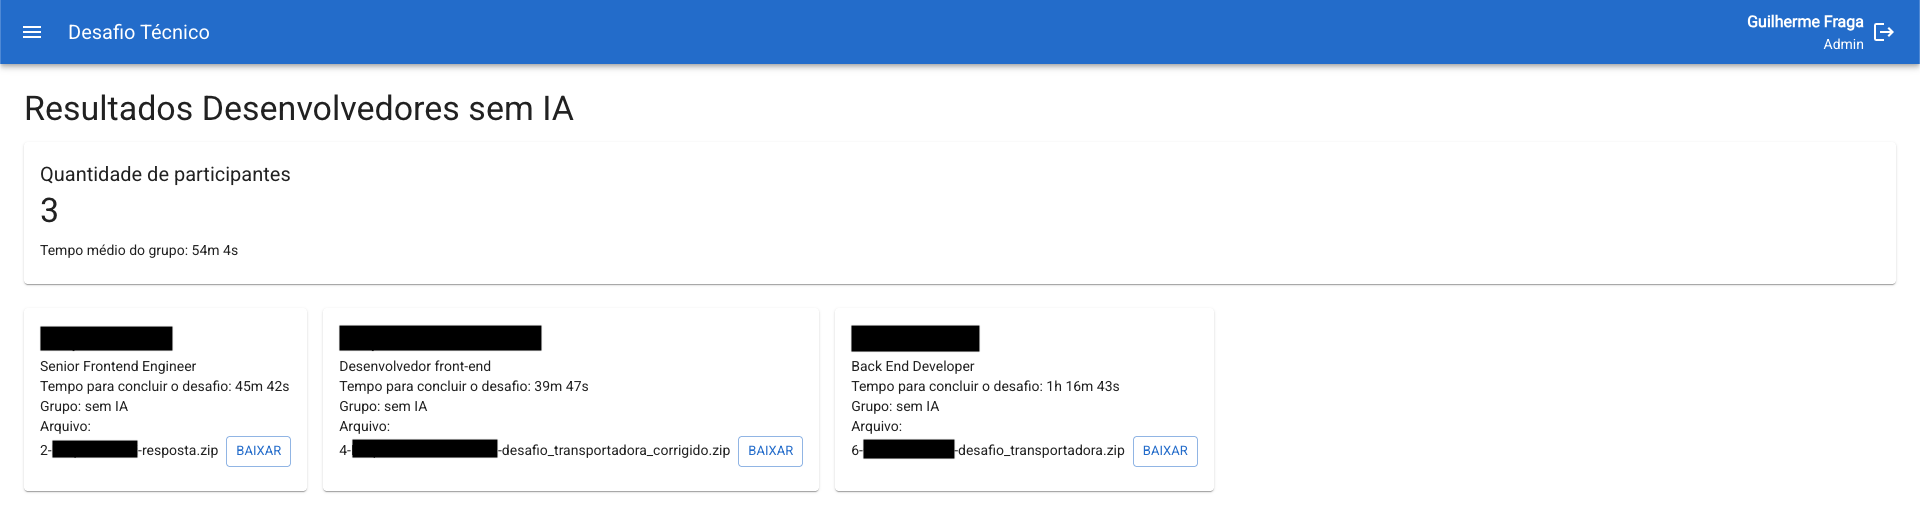
\includegraphics[width=0.95\textwidth]{images/resultados_sem_ia_admin.png}}
        \fonte{Elaborado pelo autor}
    \end{minipage}
\end{figure}
\FloatBarrier

\begin{figure}[ht]
    \caption{Resultados Desenvolvedores com IA}
    \label{fig:resultados_com_ia_admin}
    \centering
    \footnotesize
    \begin{minipage}{.9\textwidth}
        \centering
        \fbox{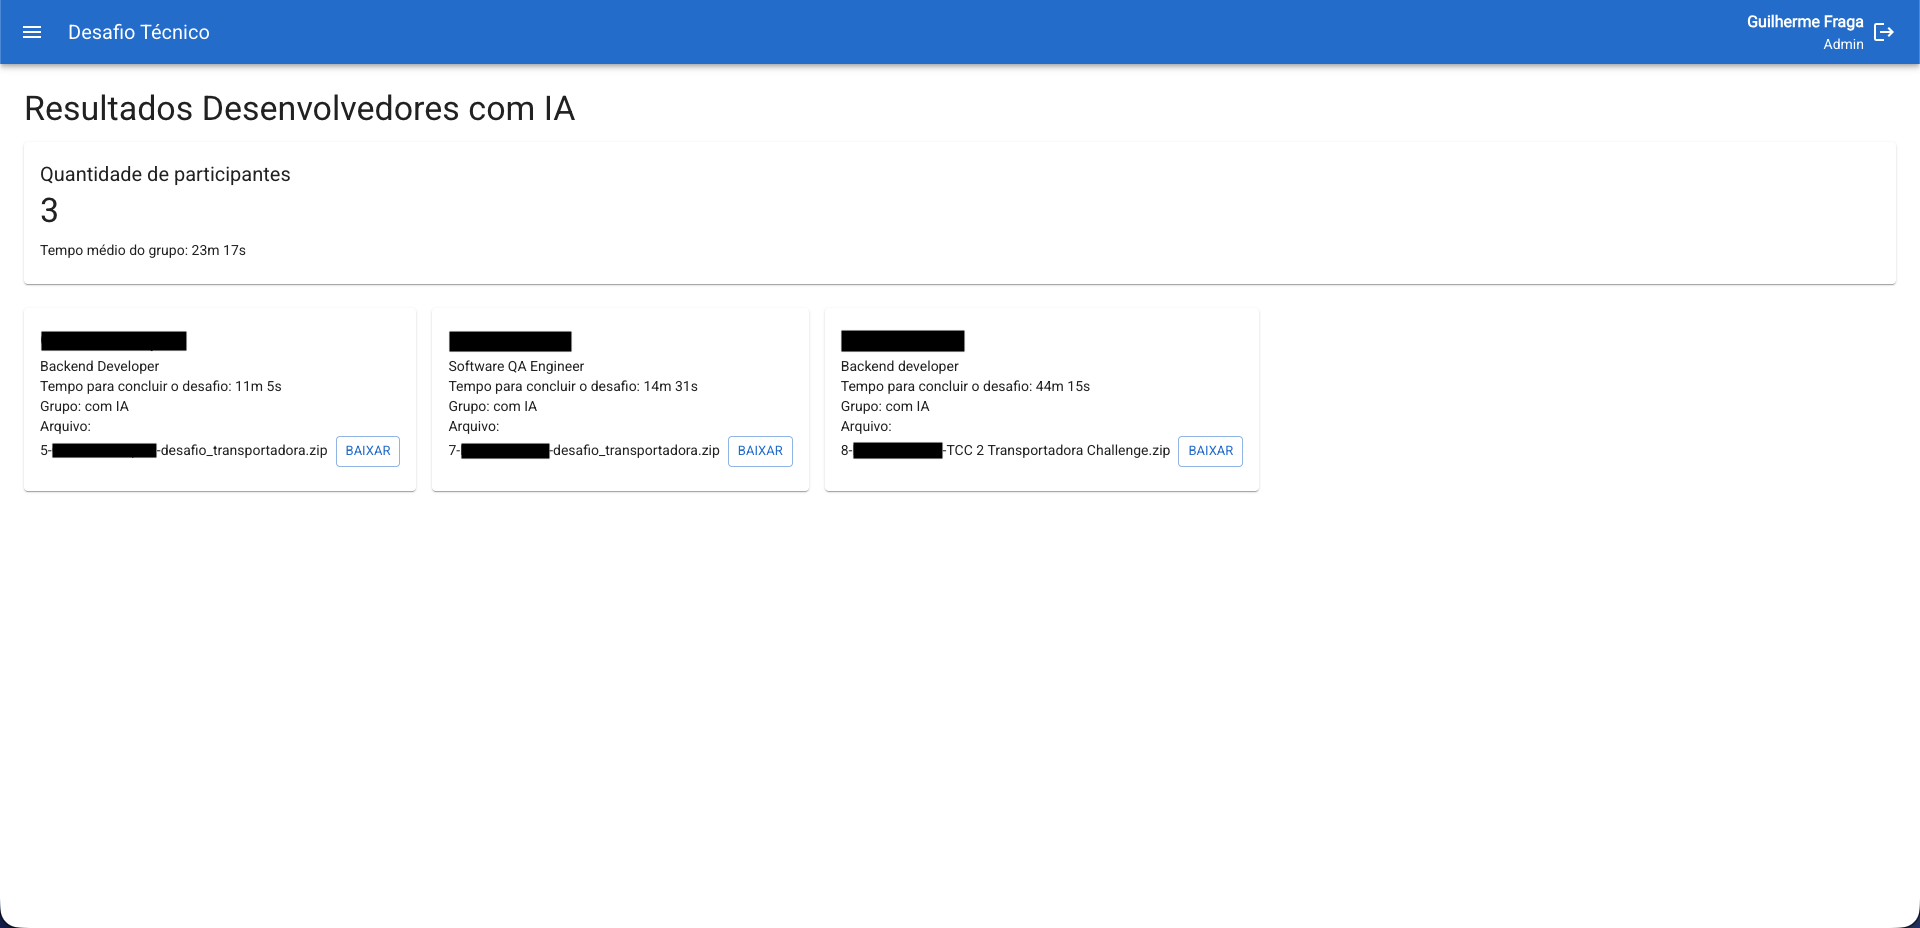
\includegraphics[width=0.95\textwidth]{images/resultados_com_ia_admin.png}}
        \fonte{Elaborado pelo autor}
    \end{minipage}
\end{figure}
\FloatBarrier

Todo o código-fonte da plataforma encontra-se disponível através do repositório\footnote{Repositório: \url{https://github.com/guifraga8/AI-Use-Productivity}} na plataforma \textit{GitHub}. Ao longo do desenvolvimento, foi utilizado o sistema de controle de versão \textit{Git}\footnote{\textit{Git}: \url{https://git-scm.com/}} para gerenciar todo o código-fonte.

\section{Análise e Discussão dos Resultados}

Nesta seção são apresentadas a coleta e análise dos dados levantados a partir das soluções fornecidas pelos participantes, juntamente com o registro do tempo total de duração para a conclusão do desafio de cada desenvolvedor. Foi coletado também dados de \textit{feedback} referente ao experimento através de um questionário aplicado no término do desafio, com o intuito de forncer mais resultados para uma análise relevante do projeto como um todo.

\subsection{Coleta de Dados}

Após a conclusão do desenvolvimento da plataforma \textit{web}, foram selecionados os participantes do experimento por conveniência, isto é, profissionais conhecidos pelo pesquisador que atuam no mercado de trabalho na área de desenvolvimento de \textit{software} e que se dispuseram a participar do desafio. Ao total foram selecionados 6 participantes. Assim, o público-alvo foi definido de forma que todos os participantes fossem da área, porém ocupando diferentes cargos, como desenvolvedor \textit{front-end}, desenvolvedor \textit{back-end}, entre outros.

Na sequência, foi realizado um sorteio com os participantes para garantir uma separação igualitária e justa entre os membros de cada grupo, denominando-os como integrantes do grupo sem IA (3 membros) ou do grupo com IA (3 membros). Em seguida, foi encaminhada, via \textit{WhatsApp}, uma mensagem individual a cada participante com as primeiras instruções, reforçando detalhes importantes para a melhor participação e validação do experimento, de acordo com o grupo definido no sorteio. Ao final da mensagem, constava o \textit{link} de acesso à plataforma (\textit{link} do grupo sem IA\footnote{\textit{Link} do grupo sem IA: \url{https://ai-use-productivity.vercel.app/register/without_ai}} e \textit{link} do grupo com IA\footnote{\textit{Link} do grupo com IA: \url{https://ai-use-productivity.vercel.app/register/with_ai}}), direcionando o participante à tela do formulário inicial. As mensagens enviadas encontram-se no Apêndice C.

Após a conclusão do desafio, isto é, após o envio da solução e finalização do mesmo (momento em que o banco de dados registrou o tempo total para a conclusão de cada desenvolvedor), cada participante foi direcionado a responder um questionário de \textit{feedback} (sendo um formulário\footnote{Formulário do grupo sem IA: \url{https://forms.gle/zdH8UPeheATCtQg67}} para o grupo sem IA e um formulário\footnote{Formulário do grupo com IA: \url{https://forms.gle/cgqkPAs93RTPuJRH9}} para o grupo com IA). Da primeira à sétima questão, o conteúdo foi igual para ambos os grupos, com o objetivo de avaliar aspectos como o nível de conhecimento da linguagem de programação (\textit{JavaScript}) proposta no desafio, a percepção individual quanto ao nível de dificuldade da atividade, o \textit{feedback} sobre a clareza do material disponibilizado para o desenvolvimento da solução, a percepção sobre o tempo demandado para resolução, além de verificar se o participante utiliza ferramentas de IA Generativa em suas atividades profissionais voltadas ao desenvolvimento de \textit{software} e, em caso afirmativo, quais.

Da oitava à décima questão, o foco recaiu sobre a abordagem adotada pelos participantes para solucionar o desafio, sendo estas perguntas diferentes para o grupo sem IA e para o grupo com IA. No grupo sem IA, questionou-se quais ferramentas foram utilizadas para auxiliar na resolução, apresentando múltiplas opções que não envolviam ferramentas de IA. Também foi solicitado um breve relato sobre como o desafio foi abordado sem o uso de IA e, por fim, pediu-se que descrevessem, em poucas palavras, sua percepção individual acerca dos obstáculos enfrentados (se houveram), considerando a restrição ao uso de ferramentas de IA Generativa.

Para o grupo com IA, as questões foram similares, porém adaptadas ao uso de ferramentas de IA Generativa na resolução do desafio. Assim, questionou-se quais ferramentas de IA foram utilizadas, foi solicitado igualmente um breve relato sobre como o desafio foi abordado com o auxílio de IA e, por fim, pediu-se que descrevessem, em poucas palavras, sua percepção individual quanto aos obstáculos enfrentados (se houveram) durante o desafio com o uso de IA Generativa.

A décima primeira questão foi comum a ambos os grupos, tendo como finalidade coletar \textit{feedbacks} adicionais dos participantes a respeito do experimento como um todo. Essa pergunta foi incluída apenas para o encerramento do questionário e para fins de obtenção de sugestões voltadas à melhoria da plataforma ou do próprio experimento, visando contribuir com trabalhos futuros na mesma linha de pesquisa. Todas as questões encontram-se no Apêndice E, e suas respectivas respostas estão apresentadas no Apêndice F.

\subsection{Avaliação dos Resultados}

A partir dos arquivos de soluções dos participantes, cada um foi analisado tomando como base os \textit{inputs} fornecidos nas imagens de exemplo dentro da plataforma e validando se o \textit{output} de cada cenário, na solução de cada desenvolvedor, correspondia ao resultado esperado. Ou seja, para cada solução, primeiramente foram realizados testes utilizando a interface \textit{HTML} do desafio, inserindo cada \textit{input} e verificando o resultado. Dessa forma, tornou-se possível identificar de maneira prática se os \textit{bugs} propositais do desafio haviam sido resolvidos. Os detalhes dos cenários de testes encontram-se disponíveis do Apêndice D.

Para cada \textit{bug} pré-estabelecido, e ao executar os cenários de teste, foram atribuídas as classificações “Concluído”, “Concluído parcialmente” ou “Não concluído”, de modo a indicar se, na solução final do desenvolvedor, todos os ajustes necessários haviam sido realizados para atender à conclusão do desafio. Esse processo foi repetido minuciosamente, percorrendo todos os \textit{bugs} pré-estabelecidos, desenvolvedor por desenvolvedor.

Nos cenários em que alguma operação não resultou no \textit{output} esperado, o trecho específico do código era analisado para determinar se o respectivo \textit{bug} havia sido concluído parcialmente ou não concluído de fato. Após essa análise, o código-fonte completo do arquivo \textit{main.js} do participante foi comparado, lado a lado, com o código-fonte completo do arquivo \textit{main.js} base do desafio (solucionado e funcional), a fim de realizar uma última análise minuciosa e verificar as alterações propostas por cada desenvolvedor, as decisões tomadas em aspectos específicos da lógica e reforçar a validação das classificações atribuídas a cada \textit{bug} anteriormente. Todos os resultados desta etapa de análise encontram-se no Apêndice H.

Com base nos procedimentos executados, foi possível constatar que, analisando o escopo total de participantes, dos 6 desenvolvedores:

\begin{itemize}[leftmargin=1cm, itemsep=0.1em, topsep=0.1em]
    \item 2 (33,33\%) concluíram 100\% dos \textit{bugs};
    \item 3 (50\%) concluíram 90\% dos \textit{bugs};
    \begin{itemize}[leftmargin=1.2cm, itemsep=0.1em, topsep=0.1em]
        \item 2 (66,67\%) concluíram 10\% dos \textit{bugs} parcialmente;
        \item 1 (33,33\%) não concluiu 10\% dos \textit{bugs};
    \end{itemize}
    \item 1 (16,67\%) concluiu 70\% dos \textit{bugs};
    \begin{itemize}[leftmargin=1.2cm, itemsep=0.1em, topsep=0.1em]
        \item 10\% dos \textit{bugs} foram concluídos parcialmente;
        \item 20\% não foram concluídos.
    \end{itemize}
\end{itemize}

Fazendo uma média com as porcentagens de "Concluídos, Concluídos parcialmente e Não concluídos" de todos os participantes, nota-se que os desenvolvedores concluíram 90\% dos \textit{bugs}, 5\% concluídos parcialmente e 5\% não foram concluídos. E por fim, o tempo médio fornecido através da plataforma, para a conclusão do desafio considerando os 6 participantes, foi de 38 minutos e 40 segundos.

Analisando somente os resultados do grupo sem IA, ou seja, no total de 3 participantes, constatou-se que:

\begin{itemize}[leftmargin=1cm, itemsep=0.1em, topsep=0.1em]
    \item 1 (33,33\%) concluiu 100\% dos \textit{bugs};
    \item 2 (66,67\%) concluíram 90\% dos \textit{bugs};
    \begin{itemize}[leftmargin=1.2cm, itemsep=0.1em, topsep=0.1em]
        \item 1 (50\%) concluiu 10\% dos \textit{bugs} parcialmente;
        \item 1 (50\%) não concluiu 10\% dos \textit{bugs}.
    \end{itemize}
\end{itemize}

A partir da média com as porcentagens somente dos participantes do grupo sem IA, nota-se que os desenvolvedores concluíram 93,33\% dos \textit{bugs}, 3,33\% concluídos parcialmente e 3,33\% não foram concluídos. O tempo médio para a conclusão do desafio do grupo sem IA foi de 54 minutos e 4 segundos.

Analisando somente os resultados do grupo com IA, igualmente no total de 3 participantes, constatou-se que:

\begin{itemize}[leftmargin=1cm, itemsep=0.1em, topsep=0.1em]
    \item 1 (33,33\%) concluiu 100\% dos \textit{bugs};
    \item 1 (33,33\%) concluiu 90\% dos \textit{bugs};
    \begin{itemize}[leftmargin=1.2cm, itemsep=0.1em, topsep=0.1em]
        \item 10\% dos \textit{bugs} foram concluídos parcialmente;
    \end{itemize}
    \item 1 (33,33\%) concluiu 70\% dos \textit{bugs};
    \begin{itemize}[leftmargin=1.2cm, itemsep=0.1em, topsep=0.1em]
        \item 10\% dos \textit{bugs} foram concluídos parcialmente;
        \item 20\% não foram concluídos.
    \end{itemize}
\end{itemize}

A partir da média somente dos participantes do grupo com IA, nota-se que os desenvolvedores concluíram 86,67\% dos \textit{bugs}, 6,67\% concluídos parcialmente e 6,67\% não foram concluídos. O tempo médio para a conclusão do desafio do grupo com IA foi de 23 minutos e 17 segundos.

A Tabela \ref{tab:resumo_resultados_participantes} foi elaborada para trazer os resultados individuais de cada participante, de forma resumida, para que seja possível exemplificar os pontos relevantes para as conclusões deste experimento.

\begin{table}[ht]
    \caption{Resumo dos resultados dos participantes}
    \label{tab:resumo_resultados_participantes}
    \centering%
    \footnotesize
    \begin{tabularx}{\textwidth}{XXXXX}
        \toprule
        \textbf{Participante} & \textbf{Cargo} & \textbf{Grupo} & \textbf{Resolução dos \textit{bugs}} & \textbf{Tempo total para conclusão} \\
        \midrule
        Desenvolvedor 1 & \textit{Senior Frontend Engineer} & sem IA & 90\% concluído, 10\% concluído parcialmente & 45m 42s \\
        \midrule
        Desenvolvedor 2 & Desenvolvedor \textit{front-end} & sem IA & 100\% concluído & 39m 47s \\
        \midrule
        Desenvolvedor 3 & \textit{Back End Developer} & sem IA & 90\% concluído, 10\% não concluído & 1h 16m 43s \\
        \midrule
        Desenvolvedor 4 & \textit{Backend Developer} & com IA & 90\% concluído, 10\% concluído parcialmente & 11m 5s \\
        \midrule
        Desenvolvedor 5 & \textit{Software QA Engineer} & com IA & 70\% concluído, 10\% concluído parcialmente, 20\% não concluído & 14m 31s \\
        \midrule
        Desenvolvedor 6 & \textit{Backend developer} & com IA & 100\% concluído & 44m 15s \\
        \bottomrule
    \end{tabularx}
    \fonte{Elaborado pelo autor}
\end{table}
\FloatBarrier

Com relação aos resultados dos questionários de \textit{feedback} solicitados aos participantes, pontua-se alguns dados interessantes, onde dos 6 desenvolvedores:

\begin{itemize}[leftmargin=1cm, itemsep=0.1em, topsep=0.1em]
    \item 6 (100\%) afirmaram já possuirem conhecimento ou experiência na linguagem \textit{JavaScript};
    \begin{itemize}[leftmargin=1.2cm, itemsep=0.1em, topsep=0.1em]
        \item 1 (16,67\%) com nível de conhecimento muito báscio;
        \item 1 (16,67\%) com nível de conhecimento básico;
        \item 3 (50\%) com nível de conhecimento avançado;
        \item 1 (16,67\%) com nível de muito avançado;
    \end{itemize}
    \item 5 (83,33\%) consideraram o desafio como fácil;
    \begin{itemize}[leftmargin=1.2cm, itemsep=0.1em, topsep=0.1em]
        \item 1 (16,67\%) considerou como neutro;
    \end{itemize}
    \item 3 (50\%) consideraram a clareza das informações do material entregue para a solução como razoável;
    \begin{itemize}[leftmargin=1.2cm, itemsep=0.1em, topsep=0.1em]
        \item 2 (33,33\%) consideraram como claro;
        \item 1 (16,67\%) considerou como muito claro;
    \end{itemize}
    \item 3 (50\%) consideraram o tamanho do desafio, com base no tempo levado para resolver, como adequado/na medida;
    \begin{itemize}[leftmargin=1.2cm, itemsep=0.1em, topsep=0.1em]
        \item 1 (16,67\%) considerou como muito rápido;
        \item 1 (16,67\%) considerou como rápido;
        \item 1 (16,67\%) considerou como demorado;
    \end{itemize}
    \item 6 (100\%) afirmaram utilizarem ferramentas de IA Generativa no dia a dia profissional relacionadas ao desenvolvimento de \textit{software};
    \begin{itemize}[leftmargin=1.2cm, itemsep=0.1em, topsep=0.1em]
        \item 3 (50\%) utilizam o \textit{ChatGPT};
        \item 2 (33,33\%) utilizam o \textit{GitHub Copilot};
        \item 1 (16,67\%) utiliza o \textit{Gemini};
        \item 3 (50\%) utilizam o \textit{Microsoft Copilot};
        \item 1 (16,67\%) utiliza o \textit{Amazon Q};
        \item 1 (16,67\%) utiliza o \textit{Cline};
        \item 1 (16,67\%) utiliza \textit{software} de autoria da empresa em que trabalha;
        \item 1 (16,67\%) utiliza o \textit{Windsurf};
        \item 1 (16,67\%) utiliza o \textit{Claude};
    \end{itemize}
\end{itemize}

Outras informações relevantes obtidas através dos questionários foi de que, dos membros do grupo sem IA, os 3 desenvolvedores (100\%) utilizaram do conhecimento prévio para a solução do desafio e destes apenas 1 (16,67\%) utilizou também da documentação oficial da linguagem para ajudá-lo. Dos membros do grupo com IA, os 3 desenvolvedores fizeram uso das ferramentas de IA que estão acostumados a utilizarem, sendo elas o \textit{ChatGPT} (66,67\%), \textit{Microsoft Copilot} (33,33\%) e \textit{Claude} (33,33\%).

Por fim, os resultados completos dos questionários de \textit{feedback} encontram-se disponíveis no Apêndice F.

\section{Considerações Finais e Trabalhos Futuros}

É inegável que, diante da rápida e constante evolução das ferramentas de Inteligência Artificial Generativa, o profissional da área de desenvolvimento de \textit{software} precisa adaptar-se ao uso dessas tecnologias, buscando maior produtividade e desempenho em suas atividades. Considerando o tempo médio de resolução do desafio técnico proposto, observou-se que o grupo que utilizou ferramentas de IA levou, em média, menos da metade do tempo em comparação ao grupo sem o uso dessas ferramentas.

Esse resultado evidencia o ganho significativo de otimização de tempo e produtividade na resolução de problemas. Entretanto, um ponto relevante observado foi que um dos desenvolvedores do grupo sem IA conseguiu concluir todas as etapas do desafio em tempo inferior ao de um participante do grupo com IA que também completou integralmente a tarefa. Isso demonstra que, apesar de o uso da IA ter contribuído para uma execução mais rápida, nem todos os participantes com acesso à ferramenta conseguiram atingir 100\% do resultado esperado.

Da mesma forma, verificou-se que o desenvolvedor do grupo com IA que solucionou completamente o desafio fez uso consciente e criterioso da ferramenta, analisando sua própria solução de forma robusta e não dependendo exclusivamente das respostas fornecidas pela IA. Essa observação foi reforçada pelas respostas do formulário de avaliação, nas quais o participante relatou que utilizou a IA como apoio para o raciocínio e não como substituto do pensamento crítico.

Por outro lado, alguns participantes do grupo sem IA aparentemente não realizaram uma verificação detalhada de suas soluções. Assim, destaca-se a importância de que, mesmo com o auxílio de ferramentas de IA, o desenvolvedor mantenha uma postura analítica e revisora, garantindo que o resultado final atenda integralmente aos requisitos propostos, com clareza e qualidade.

Ressalta-se, portanto, que as ferramentas de IA Generativas são grandes aliadas do desenvolvedor moderno, desde que utilizadas de forma equilibrada. O uso responsável dessas tecnologias deve reforçar e, não substituir, o conhecimento técnico e o senso crítico do profissional. Afinal, trata-se de ferramentas ainda em processo de evolução, mesmo que esse avanço ocorra em ritmo acelerado.

Essa relação de complementaridade entre desenvolvedor e IA Generativa também ficou evidente nas respostas dos participantes do grupo sem IA, que apontaram como principais desafios a ausência de recursos como o \textit{autocomplete} e a dificuldade em realizar pesquisas e revisões de código sem o suporte de IA. Um dos desenvolvedores, inclusive, destacou que, antes do experimento, acreditava ser plenamente capaz de desenvolver sem o uso de IA, mas, após a experiência, percebeu o quanto o processo se torna mais demorado e trabalhoso sem essas ferramentas.

Esses relatos reforçam a percepção de que as ferramentas de IA Generativas se tornaram parte essencial do cotidiano dos desenvolvedores, contribuindo diretamente para a performance, a otimização de tempo e a praticidade em tarefas rotineiras. Contudo, é fundamental que seu uso seja feito de forma consciente, evitando dependências que possam limitar a autonomia e o raciocínio do profissional.

Em relação ao experimento realizado, os \textit{feedbacks} dos participantes indicaram a necessidade de maior clareza na descrição do desafio técnico. Sugere-se que, em futuras aplicações, os exemplos de \textit{inputs} e \textit{outputs} sejam fornecidos em formato textual, e não apenas em imagens, permitindo que os desenvolvedores possam copiar e testar diretamente as informações, evitando erros e retrabalhos.

Por fim, destaca-se que seria relevante repetir o experimento com uma amostra maior de participantes, possibilitando uma análise mais ampla e representativa sobre o impacto real do uso e da ausência de ferramentas de IA Generativa no desempenho de desenvolvedores de \textit{software}. Outra sugestão de melhoria para aplicações futuras seria a de, ao realizar um experimento desse tipo, mensurar não apenas o tempo e a capacidade de resolução do desafio técnico, mas também aspectos técnicos relacionados à qualidade das soluções entregues. Isso incluiria critérios como a clareza e organização do código, nível de otimização, boas práticas aplicadas, modularização, bem como a análise de complexidade (melhor caso, pior caso e caso médio). Dessa forma, seria possível realizar uma comparação mais abrangente entre os grupos que utilizaram ferramentas de IA e aqueles que não utilizaram, permitindo avaliar não apenas a produtividade, mas também a qualidade técnica das soluções geradas.

Como proposta para trabalhos futuros, além das sugestões acima, seria interessante aplicar novos desafios técnicos envolvendo grupos com e sem IA, em que os participantes com IA não necessariamente sejam desenvolvedores ativos, mas profissionais da área de tecnologia em diferentes funções. Dessa forma, seria possível avaliar o impacto do uso de IA também em profissionais com conhecimento básico em lógica e programação, mas com perfis distintos, ampliando o entendimento sobre o potencial e os limites da IA Generativa em diferentes contextos de atuação.

\bibliography{references}

\appendix
\section{DIAGRAMA ER DO BANCO DE DADOS}

\renewcommand{\thefigure}{A.\arabic{figure}}
\setcounter{figure}{0}

\begin{figure}[ht]
    \caption{Modelo Entidade Relacional da aplicação}
    \vspace{1em}
    \label{fig:diagrama_er_banco}
    \centering%
    \footnotesize
	\begin{minipage}{.9\textwidth}
		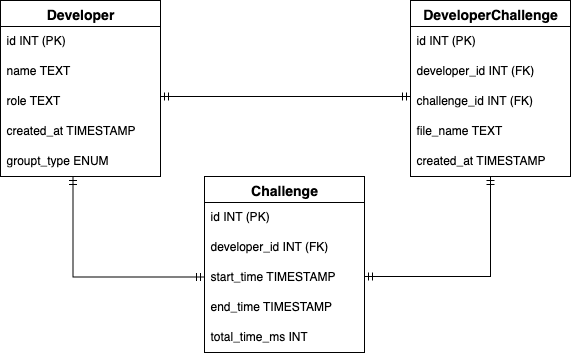
\includegraphics[width=\textwidth]{images/diagrama_er_banco.png}
		\fonte{Elaborado pelo autor}
	\end{minipage}
\end{figure}
\FloatBarrier

\section{TELAS DA APLICAÇÃO}

\renewcommand{\thefigure}{B.\arabic{figure}}
\setcounter{figure}{0}

\begin{figure}[ht]
    \caption{Exemplo 1 do desafio}
    \label{fig:exemplo1}
    \centering
    \footnotesize
    \begin{minipage}{.9\textwidth}
        \centering
        \fbox{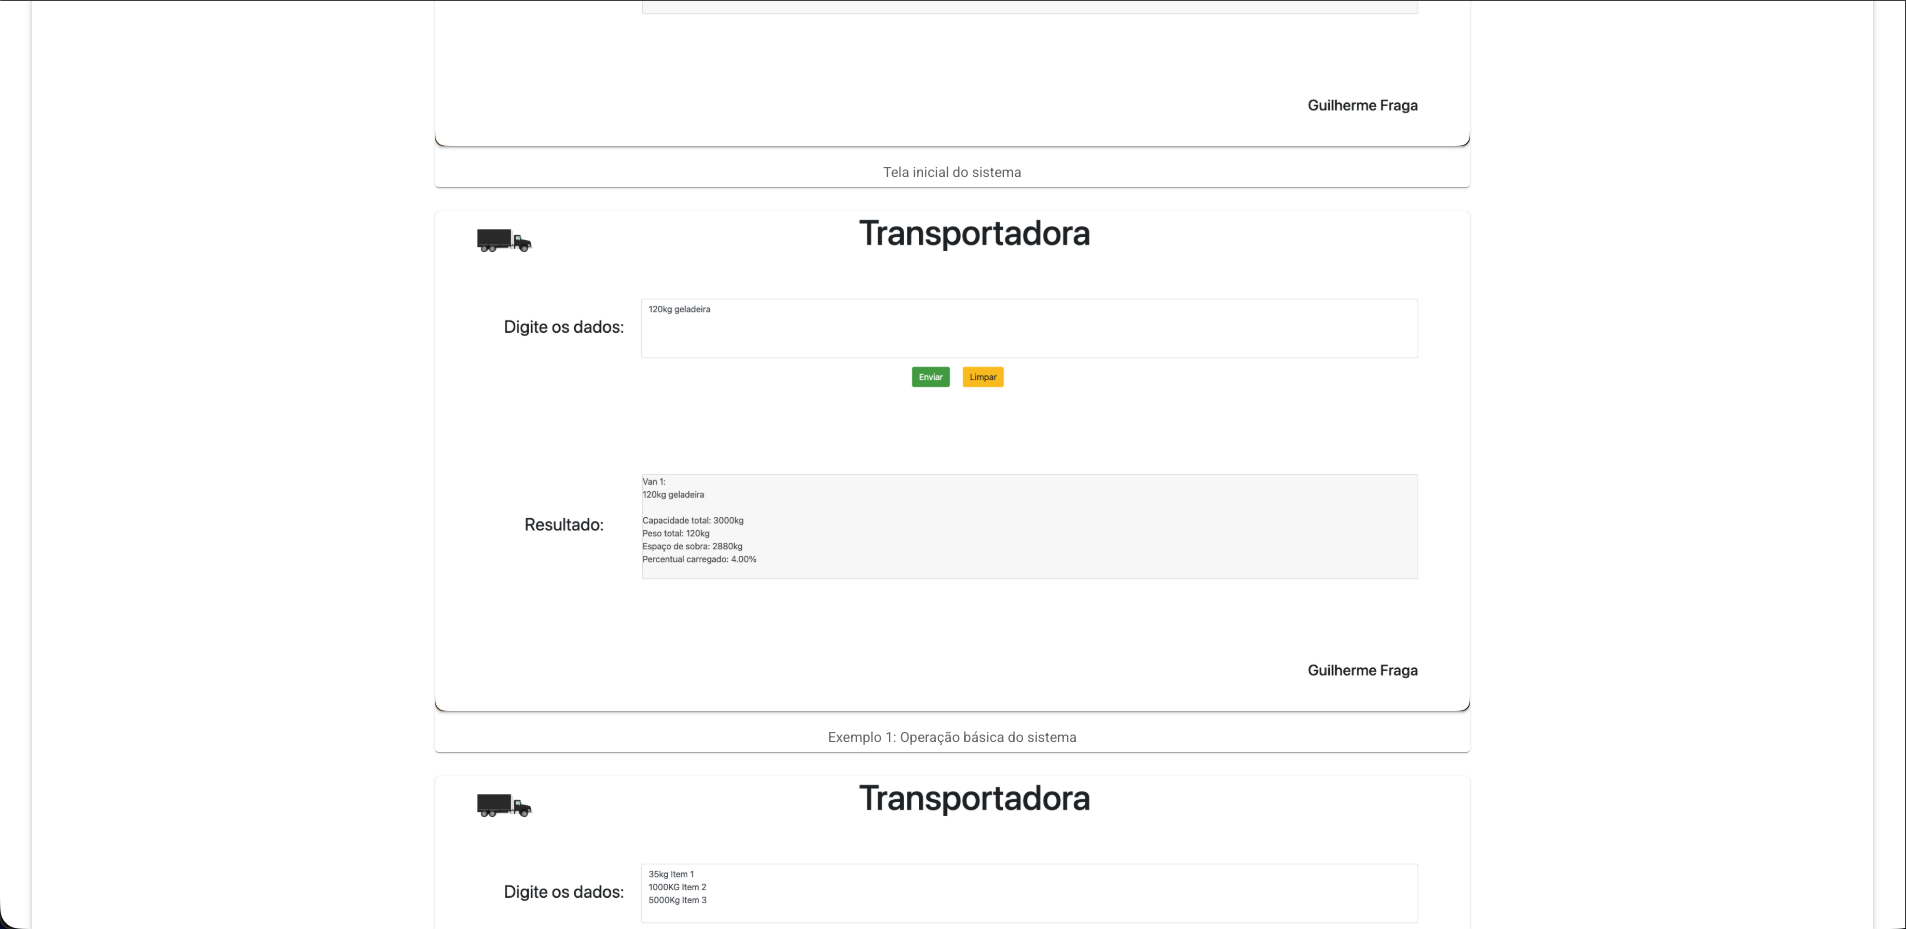
\includegraphics[width=0.95\textwidth]{images/exemplo1.png}}
        \fonte{Elaborado pelo autor}
    \end{minipage}
\end{figure}
\FloatBarrier

\begin{figure}[ht]
    \caption{Exemplo 2 do desafio}
    \label{fig:exemplo2}
    \centering
    \footnotesize
    \begin{minipage}{.9\textwidth}
        \centering
        \fbox{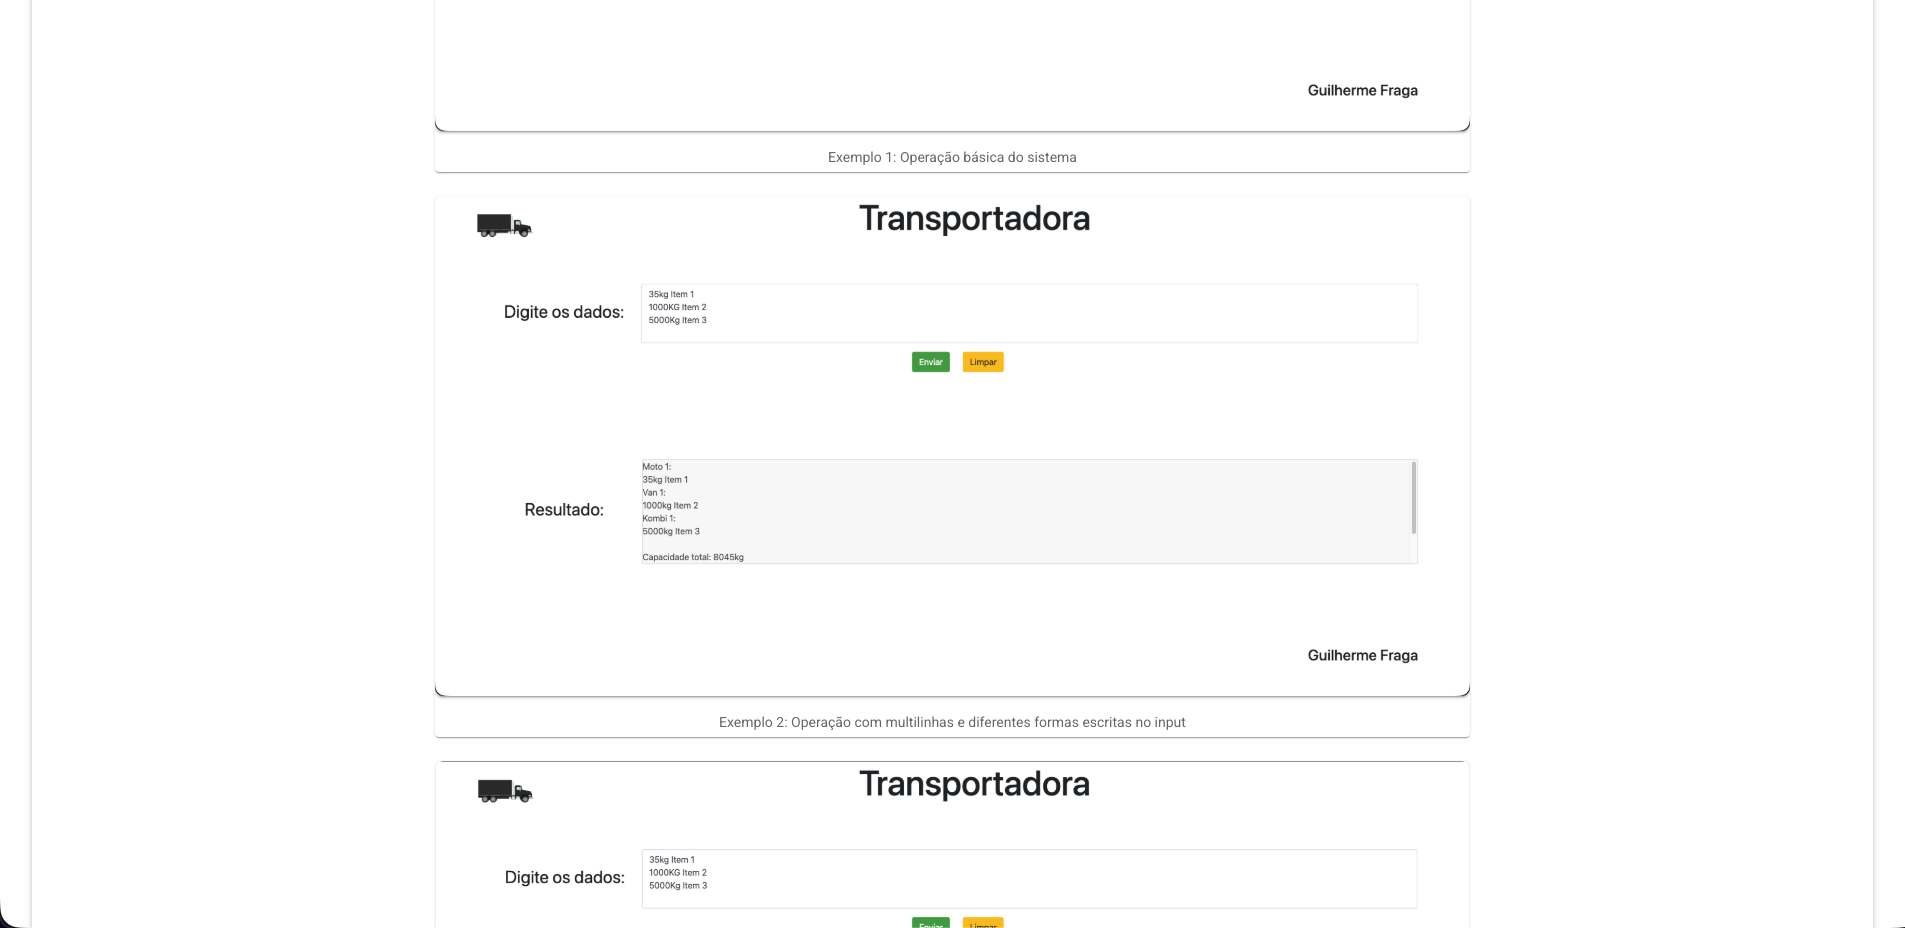
\includegraphics[width=0.95\textwidth]{images/exemplo2.png}}
        \fonte{Elaborado pelo autor}
    \end{minipage}
\end{figure}
\FloatBarrier

\begin{figure}[ht]
    \caption{Exemplo 2.1 do desafio}
    \label{fig:exemplo2_1}
    \centering
    \footnotesize
    \begin{minipage}{.9\textwidth}
        \centering
        \fbox{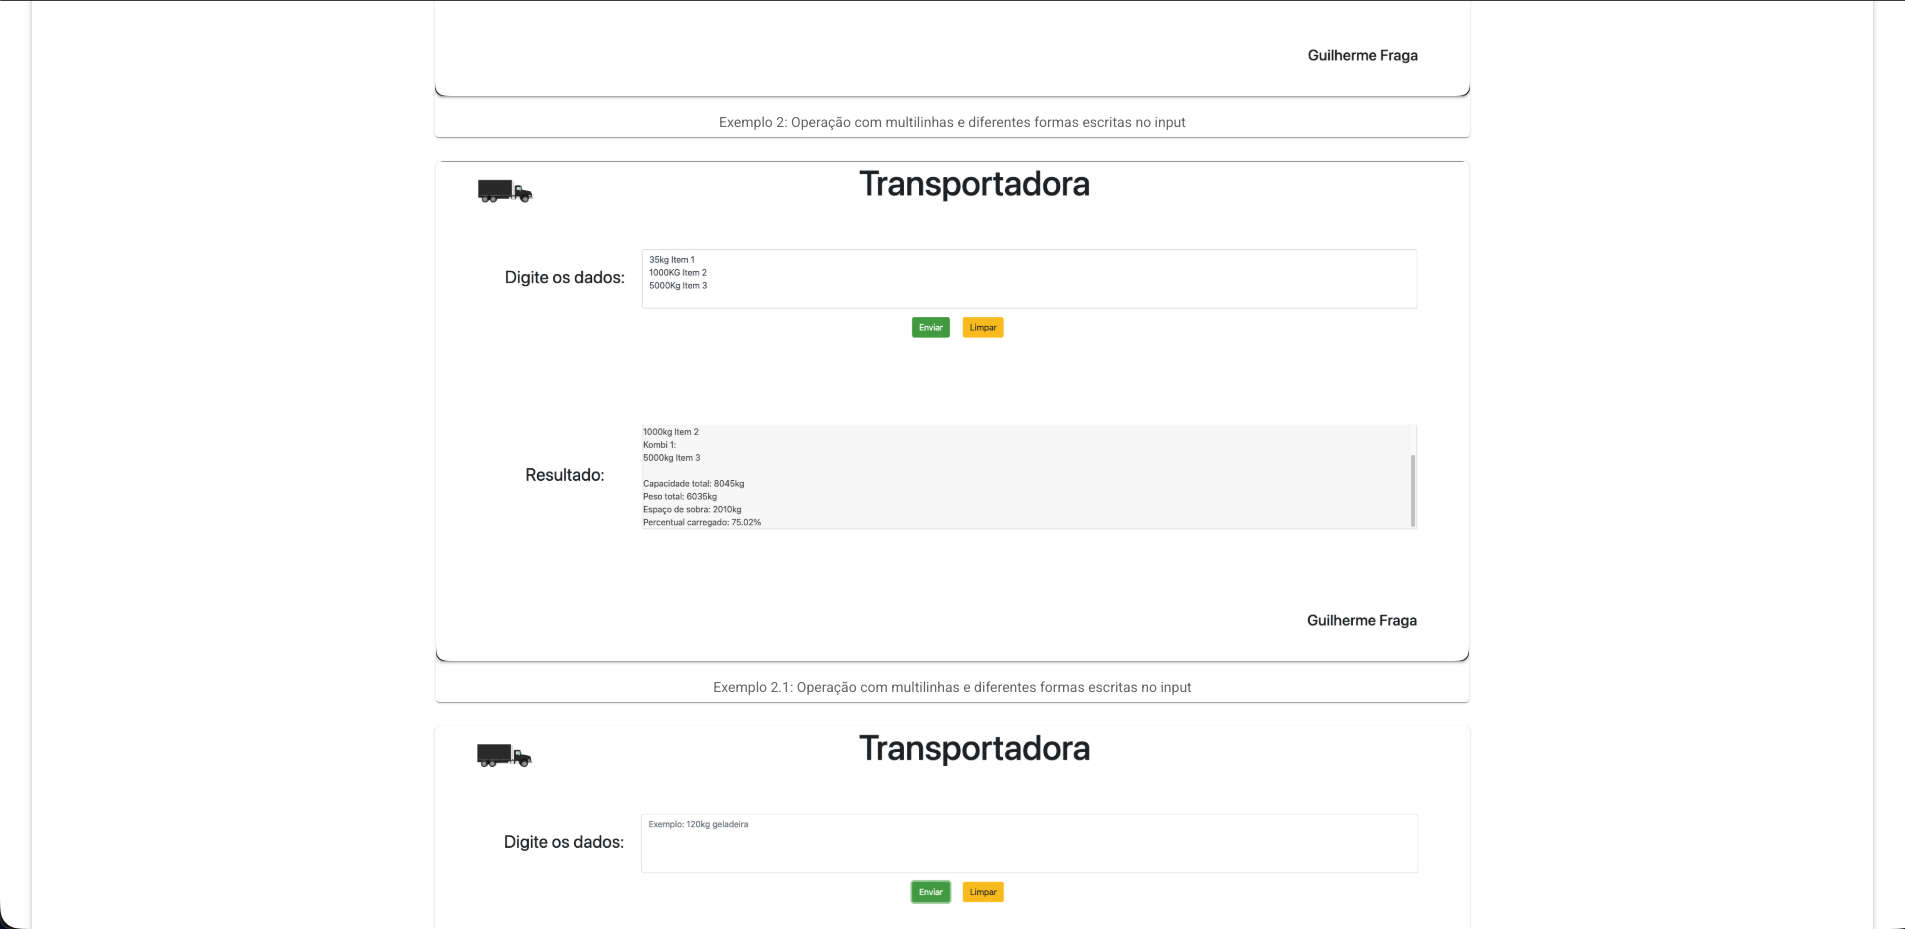
\includegraphics[width=0.95\textwidth]{images/exemplo2.1.png}}
        \fonte{Elaborado pelo autor}
    \end{minipage}
\end{figure}
\FloatBarrier

\begin{figure}[ht]
    \caption{Exemplo 3 do desafio}
    \label{fig:exemplo3}
    \centering
    \footnotesize
    \begin{minipage}{.9\textwidth}
        \centering
        \fbox{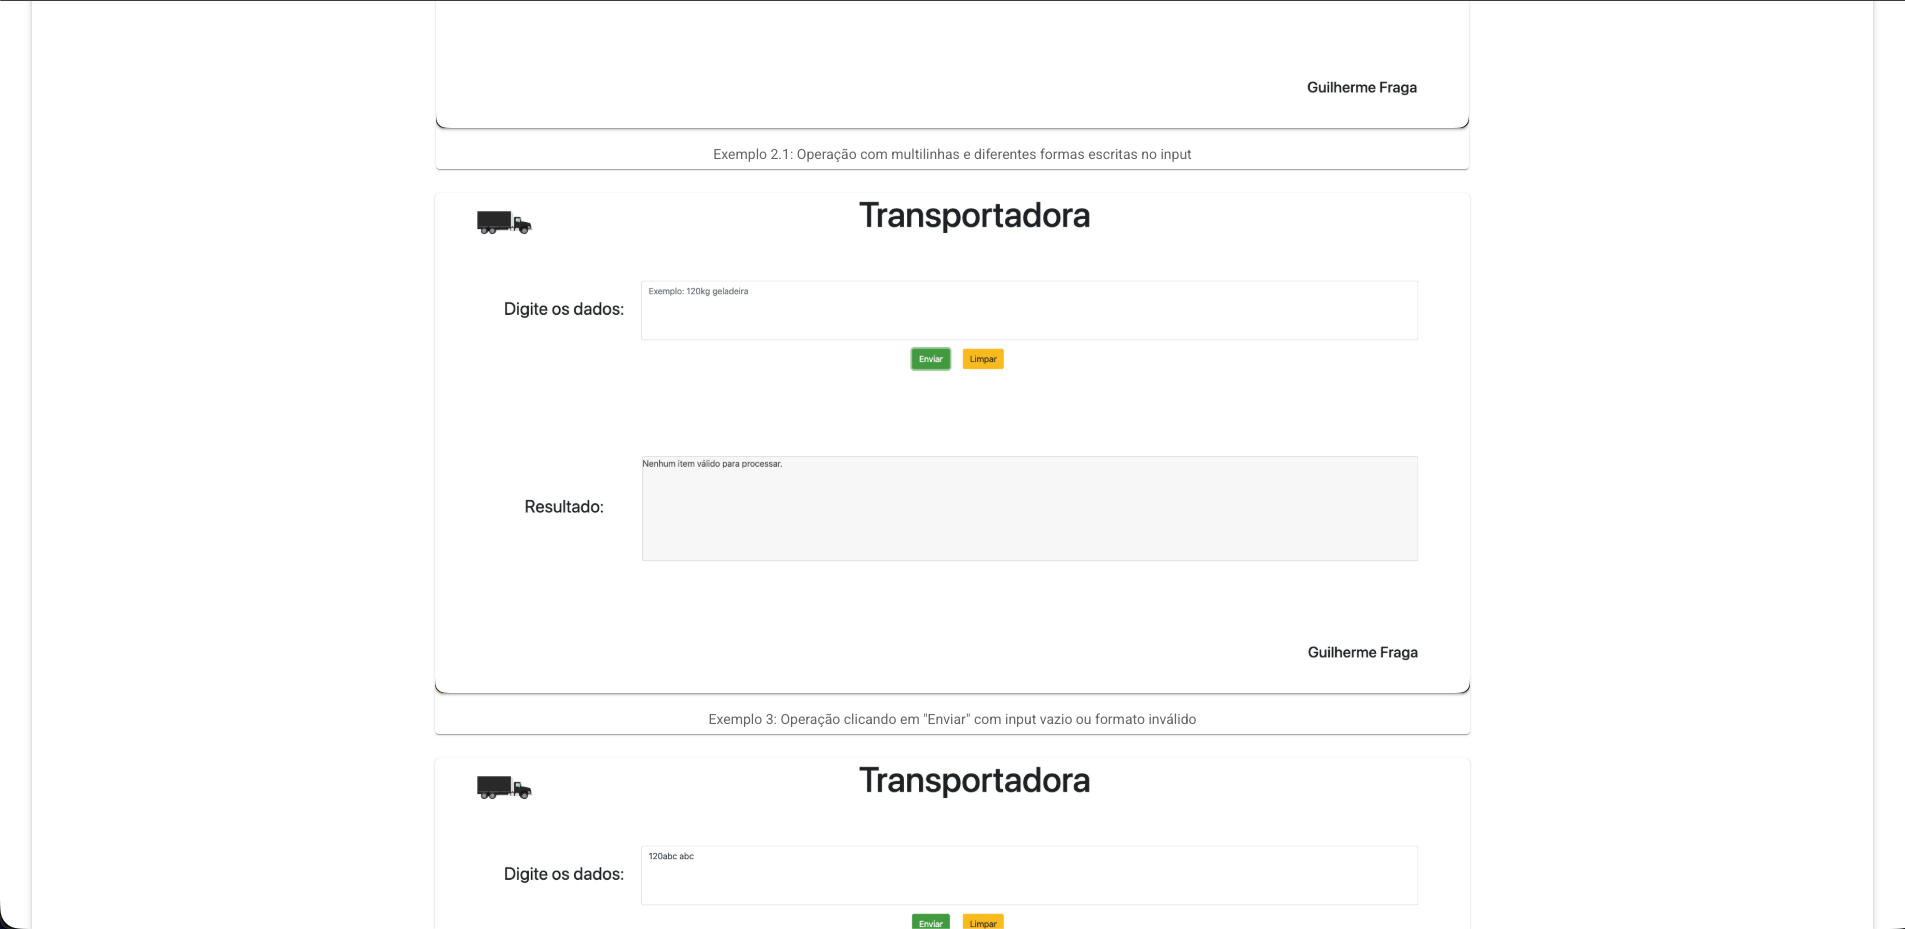
\includegraphics[width=0.95\textwidth]{images/exemplo3.png}}
        \fonte{Elaborado pelo autor}
    \end{minipage}
\end{figure}
\FloatBarrier

\begin{figure}[ht]
    \caption{Exemplo 3.1 do desafio}
    \label{fig:exemplo3_1}
    \centering
    \footnotesize
    \begin{minipage}{.9\textwidth}
        \centering
        \fbox{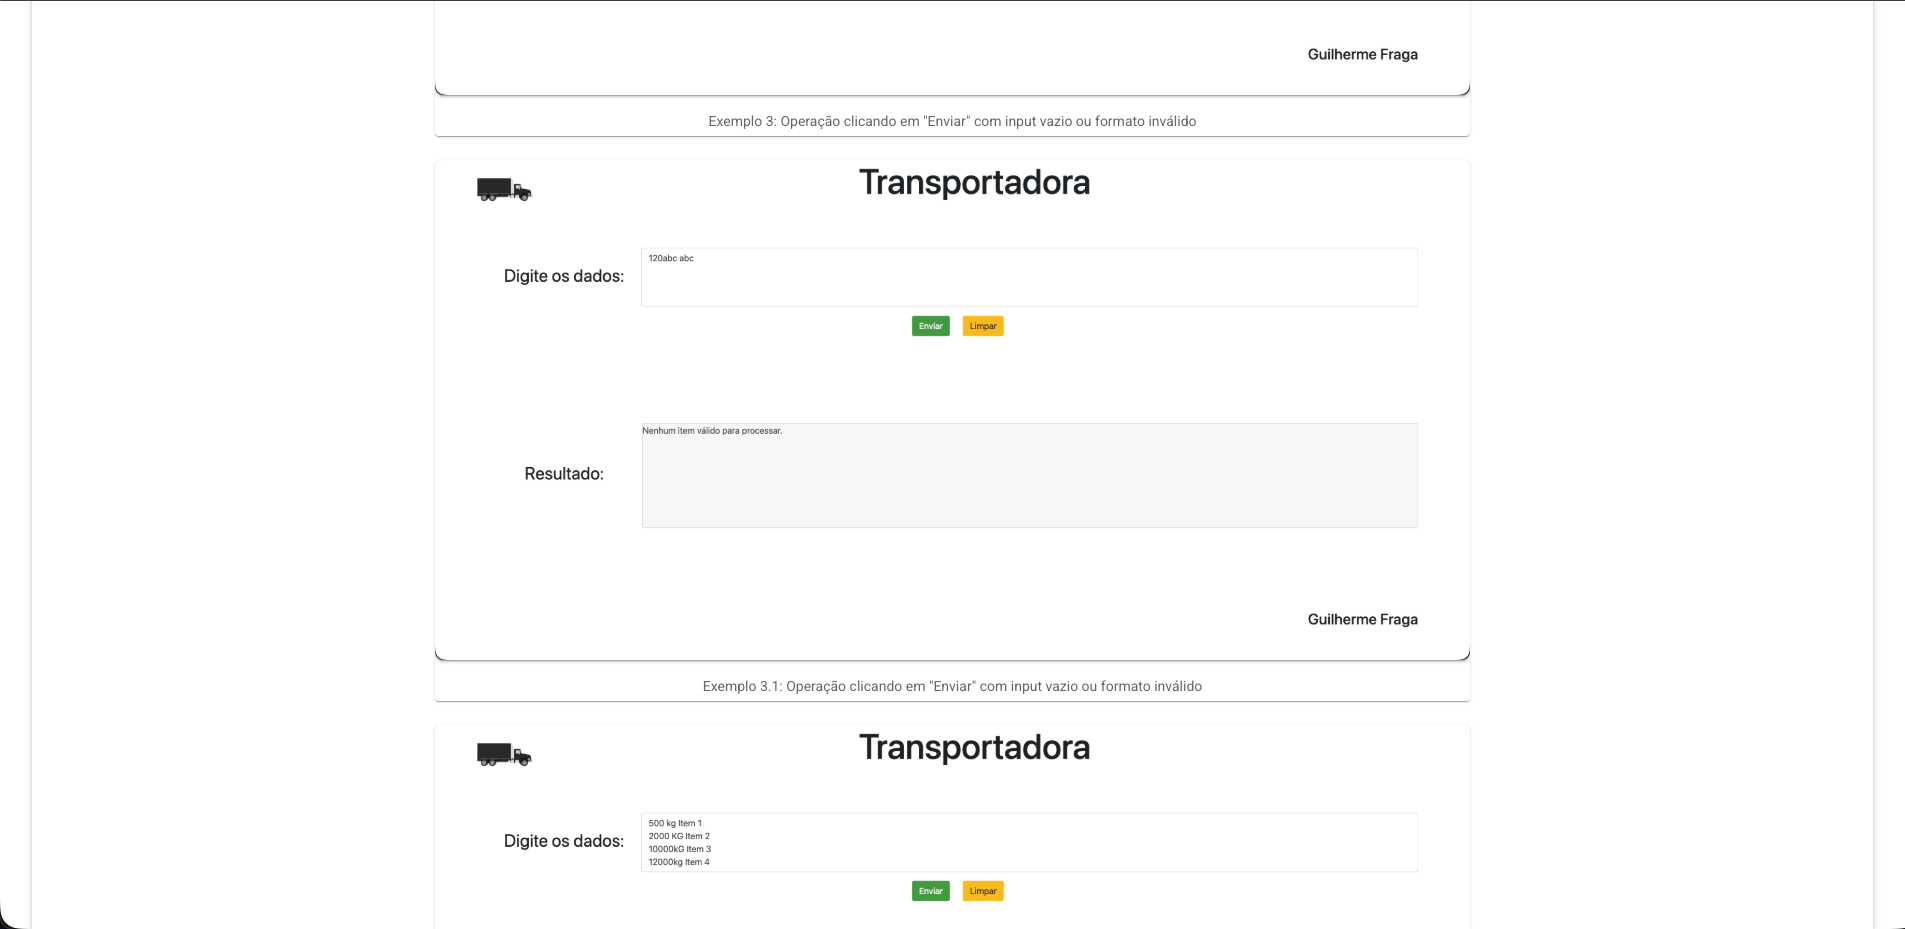
\includegraphics[width=0.95\textwidth]{images/exemplo3.1.png}}
        \fonte{Elaborado pelo autor}
    \end{minipage}
\end{figure}
\FloatBarrier

\begin{figure}[ht]
    \caption{Exemplo 4 do desafio}
    \label{fig:exemplo4}
    \centering
    \footnotesize
    \begin{minipage}{.9\textwidth}
        \centering
        \fbox{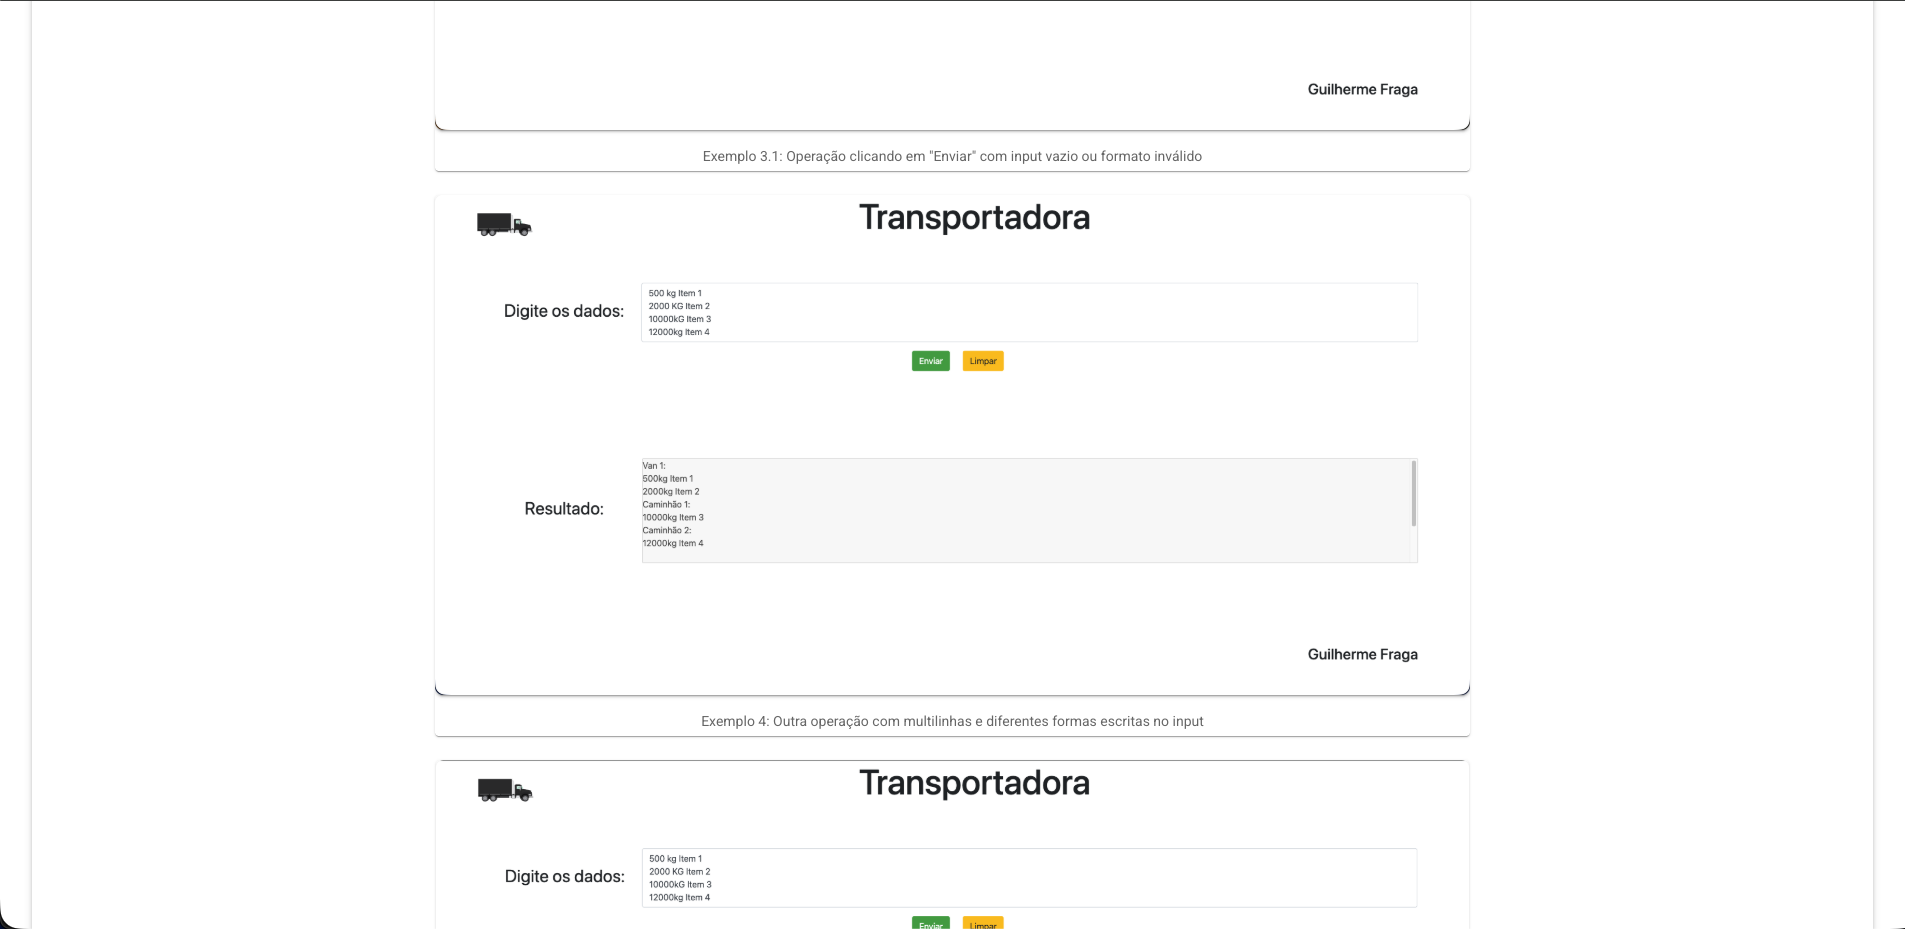
\includegraphics[width=0.95\textwidth]{images/exemplo4.png}}
        \fonte{Elaborado pelo autor}
    \end{minipage}
\end{figure}
\FloatBarrier

\begin{figure}[ht]
    \caption{Exemplo 4.1 do desafio}
    \label{fig:exemplo4_1}
    \centering
    \footnotesize
    \begin{minipage}{.9\textwidth}
        \centering
        \fbox{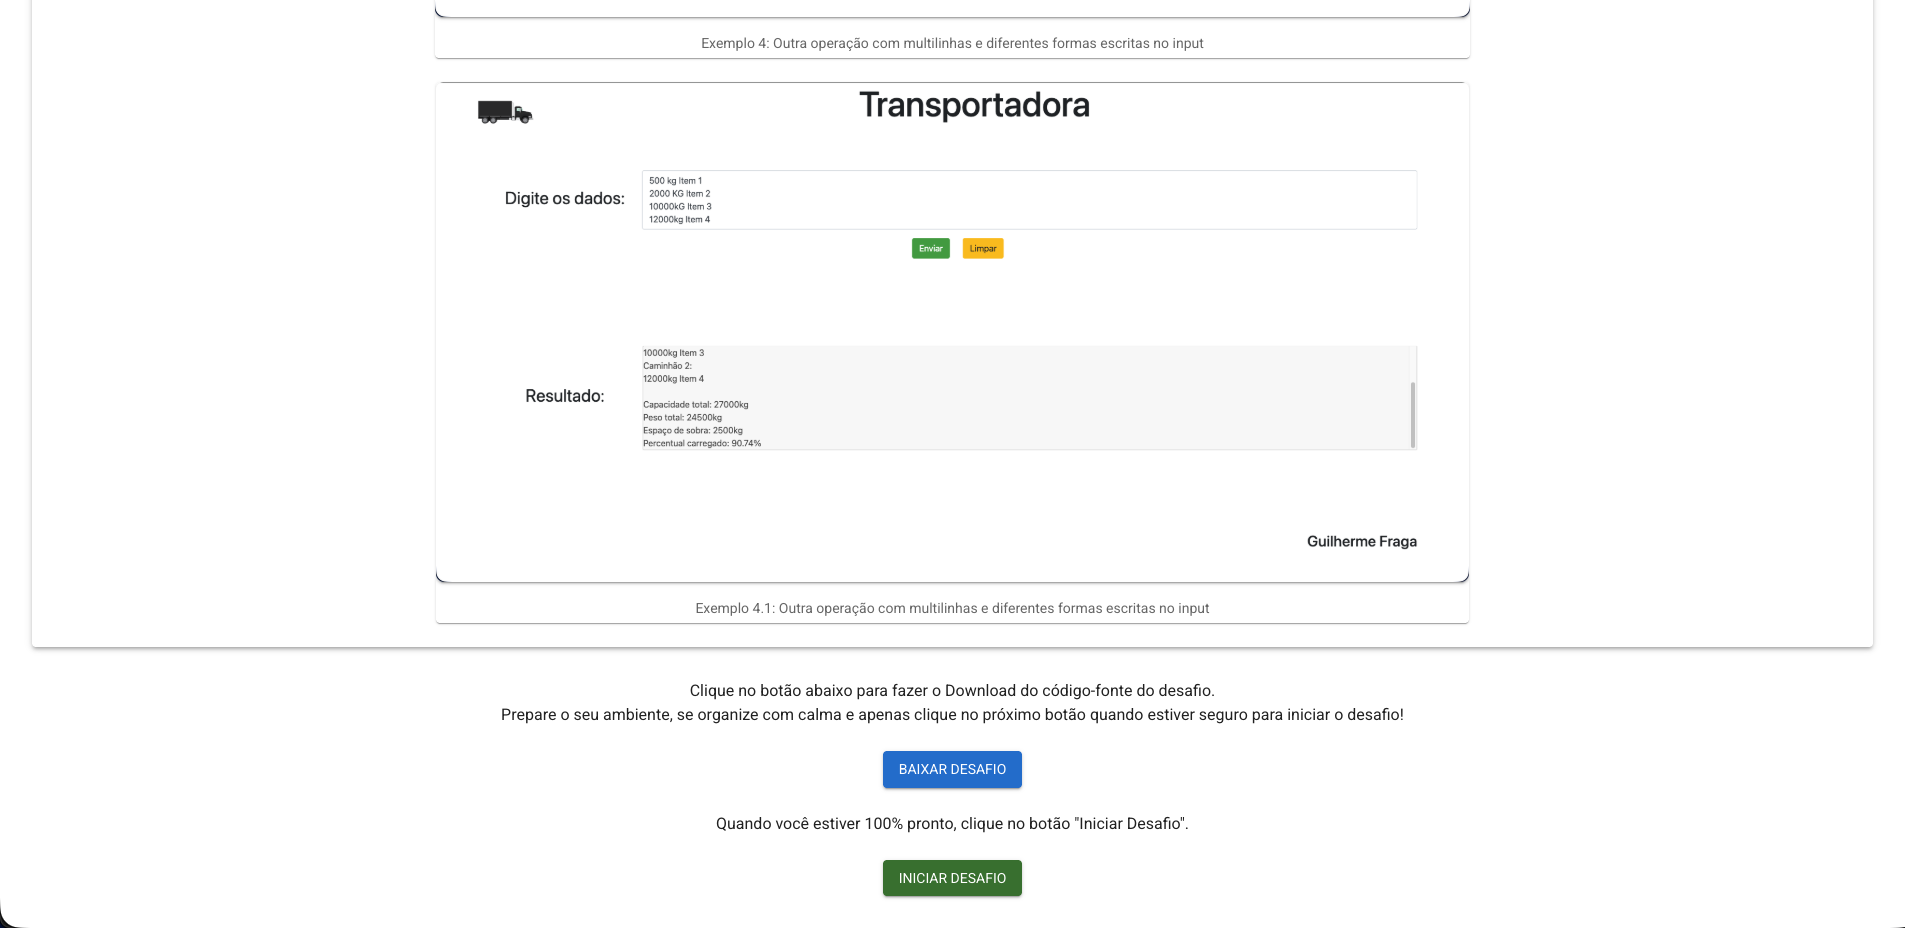
\includegraphics[width=0.95\textwidth]{images/exemplo4.1.png}}
        \fonte{Elaborado pelo autor}
    \end{minipage}
\end{figure}
\FloatBarrier

\begin{figure}[ht]
    \caption{Editar arquivo e finalizar desafio}
    \label{fig:arquivo_salvo_finalizar_desafio}
    \centering
    \footnotesize
    \begin{minipage}{.9\textwidth}
        \centering
        \fbox{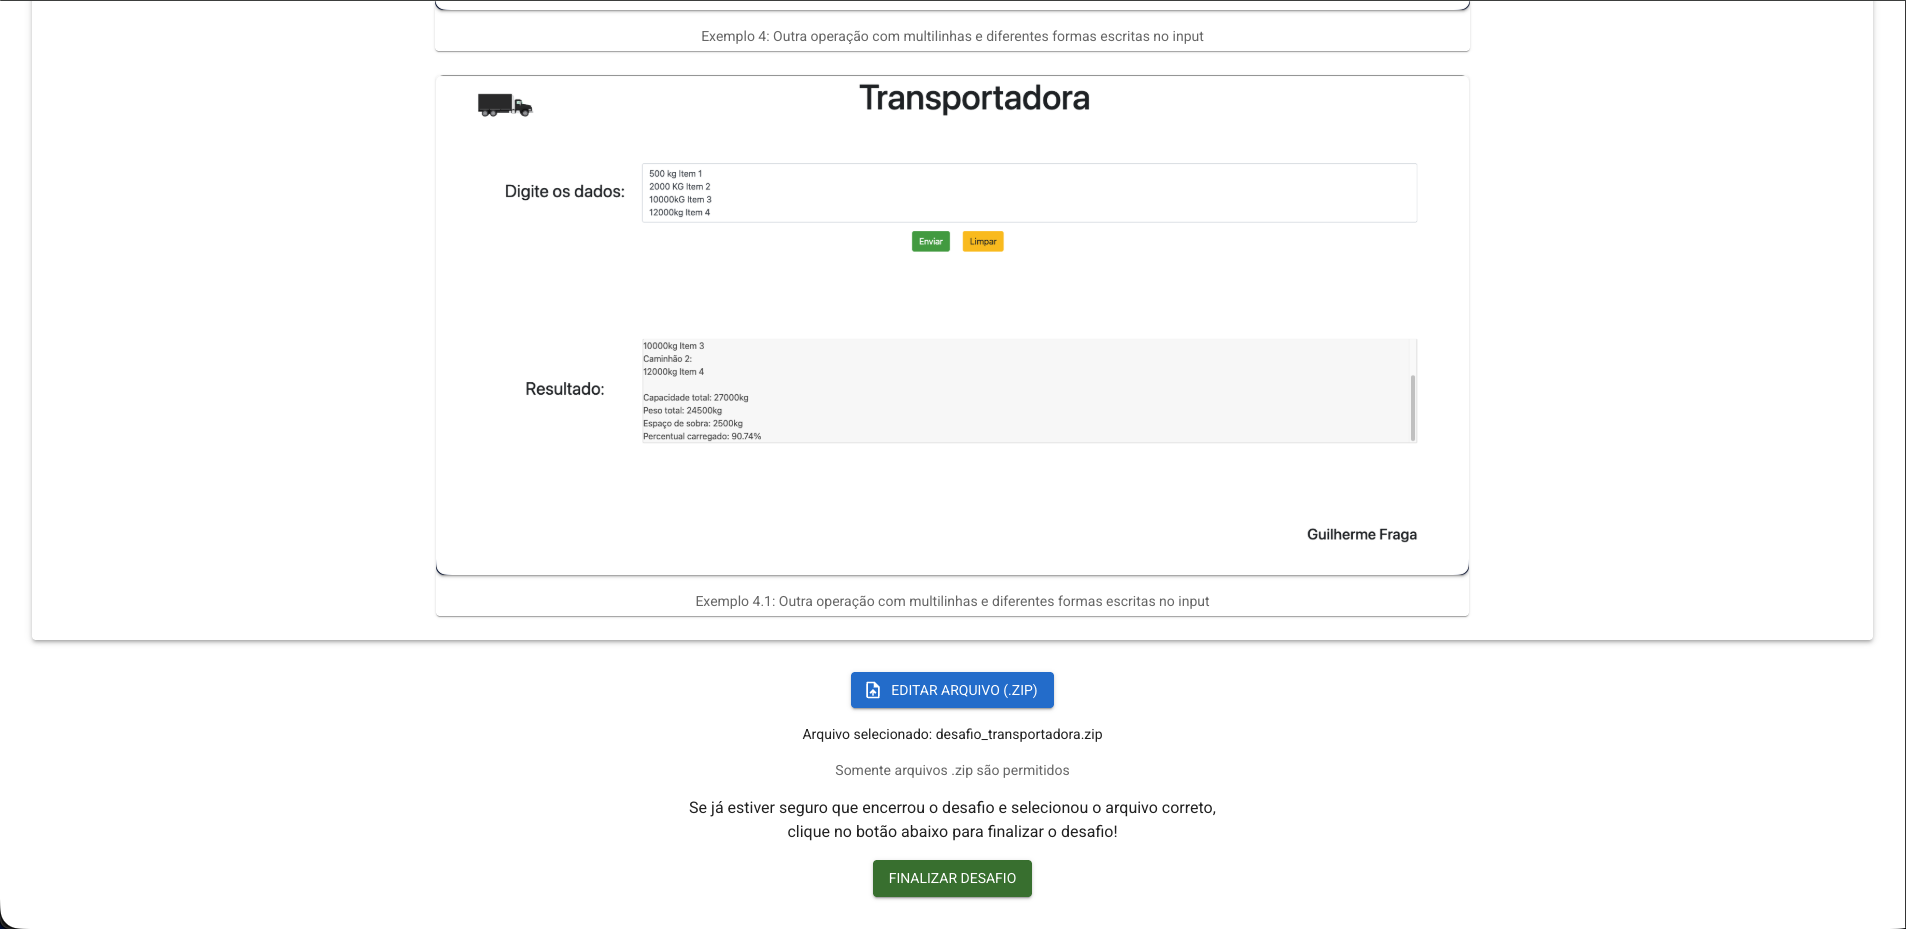
\includegraphics[width=0.95\textwidth]{images/arquivo_salvo_finalizar_desafio.png}}
        \fonte{Elaborado pelo autor}
    \end{minipage}
\end{figure}
\FloatBarrier

\section{INSTRUÇÕES ENVIADAS AOS PARTICIPANTES VIA \textit{WHATSAPP}}

\renewcommand{\thefigure}{C.\arabic{figure}}
\setcounter{figure}{0}

\begin{figure}[ht]
    \caption{Instruções enviadas via \textit{WhatsApp} para o grupo sem IA}
    \label{fig:instrucoes_sem_ia}
    \centering
    \footnotesize
    \begin{minipage}{.9\textwidth}
        \centering
        \fbox{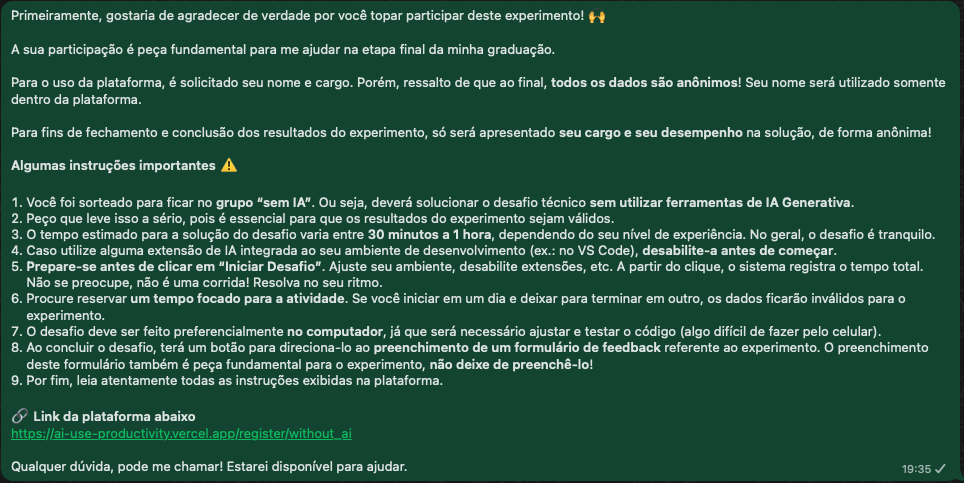
\includegraphics[width=0.95\textwidth]{images/instrucoes_sem_ia.png}}
        \fonte{Elaborado pelo autor}
    \end{minipage}
\end{figure}
\FloatBarrier

\begin{figure}[ht]
    \caption{Instruções enviadas via \textit{WhatsApp} para o grupo com IA}
    \label{fig:instrucoes_com_ia}
    \centering
    \footnotesize
    \begin{minipage}{.9\textwidth}
        \centering
        \fbox{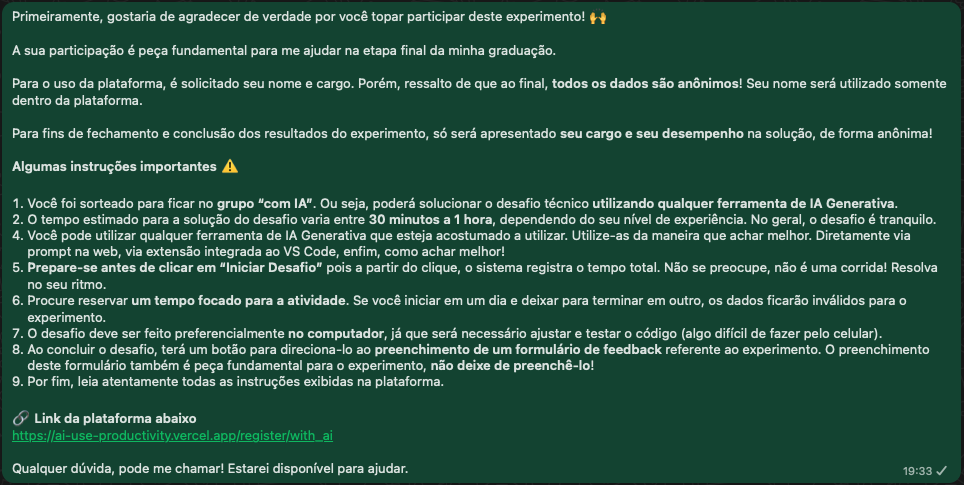
\includegraphics[width=0.95\textwidth]{images/instrucoes_com_ia.png}}
        \fonte{Elaborado pelo autor}
    \end{minipage}
\end{figure}
\FloatBarrier

\section{CENÁRIOS DE TESTES}

O desenvolvedor deveria replicar os \textit{inputs} exibidos nas imagens de exemplo, que representavam os resultados esperados no \textit{output}. Estes foram os \textit{inputs} aplicados ao testes na interface \textit{HTML} e comparado com o código-fonte base funcional para verificar se os resultados estavam coerentes.

\textbf{Cenário 1}

\begin{itemize}[leftmargin=1cm, itemsep=0.1em, topsep=0.1em]
    \item \textit{input}
    \begin{itemize}[leftmargin=1.2cm, itemsep=0.1em, topsep=0.1em]
        120kg geladeira
    \end{itemize}
    \item \textit{output}
    \begin{itemize}[leftmargin=1.2cm, itemsep=0.1em, topsep=0.1em]
        Van 1:\\
        120kg geladeira\\
        
        \\Capacidade total: 3000kg\\
        Peso total: 120kg\\
        Espaço de sobra: 2880kg\\
        Percentual carregado: 4.00\%
    \end{itemize}
\end{itemize}

\textbf{Cenário 2}

\begin{itemize}[leftmargin=1cm, itemsep=0.1em, topsep=0.1em]
    \item \textit{input}
    \begin{itemize}[leftmargin=1.2cm, itemsep=0.1em, topsep=0.1em]
        35kg Item 1\\
        1000KG Item 2\\
        5000Kg Item 3
    \end{itemize}
    \item \textit{output}
    \begin{itemize}[leftmargin=1.2cm, itemsep=0.1em, topsep=0.1em]
        Moto 1:\\
        35kg Item 1\\
        Van 1:\\ 
        1000kg Item 2\\
        Kombi 1:\\
        5000kg Item 3\\

        \\Capacidade total: 8045kg\\
        Peso total: 6035kg\\
        Espaço de sobra: 2010kg\\
        Percentual carregado: 75.02\%
    \end{itemize}
\end{itemize}

\textbf{Cenário 3}

\begin{itemize}[leftmargin=1cm, itemsep=0.1em, topsep=0.1em]
    \item \textit{input}
    \begin{itemize}[leftmargin=1.2cm, itemsep=0.1em, topsep=0.1em]
        vazio
    \end{itemize}
    \item \textit{output}
    \begin{itemize}[leftmargin=1.2cm, itemsep=0.1em, topsep=0.1em]
        Nenhum item válido para processar.
    \end{itemize}
\end{itemize}

\textbf{Cenário 4}

\begin{itemize}[leftmargin=1cm, itemsep=0.1em, topsep=0.1em]
    \item \textit{input}
    \begin{itemize}[leftmargin=1.2cm, itemsep=0.1em, topsep=0.1em]
        120abc abc
    \end{itemize}
    \item \textit{output}
    \begin{itemize}[leftmargin=1.2cm, itemsep=0.1em, topsep=0.1em]
        Nenhum item válido para processar.
    \end{itemize}
\end{itemize}

\textbf{Cenário 5}

\begin{itemize}[leftmargin=1cm, itemsep=0.1em, topsep=0.1em]
    \item \textit{input}
    \begin{itemize}[leftmargin=1.2cm, itemsep=0.1em, topsep=0.1em]
        500 kg Item 1\\
        2000 KG Item 2\\
        10000kG Item 3\\
        12000kg Item 4
    \end{itemize}
    \item \textit{output}
    \begin{itemize}[leftmargin=1.2cm, itemsep=0.1em, topsep=0.1em]
        Van 1:\\
        500kg Item 1\\
        2000kg Item 2\\
        Caminhão 1:\\
        10000kg Item 3\\
        Caminhão 2:\\
        12000kg Item 4\\

        \\Capacidade total: 27000kg\\
        Peso total: 24500kg\\
        Espaço de sobra: 2500kg\\
        Percentual carregado: 90.74\%
    \end{itemize}
\end{itemize}

\section{QUESTIONÁRIOS DE AVALIAÇÃO DO MODELO}

\renewcommand{\thefigure}{E.\arabic{figure}}
\setcounter{figure}{0}

\begin{figure}[ht]
    \caption{Questão 1 e 2 do formulário final para todos os participantes}
    \label{fig:questao1_2_geral}
    \centering
    \footnotesize
    \begin{minipage}{.9\textwidth}
        \centering
        \fbox{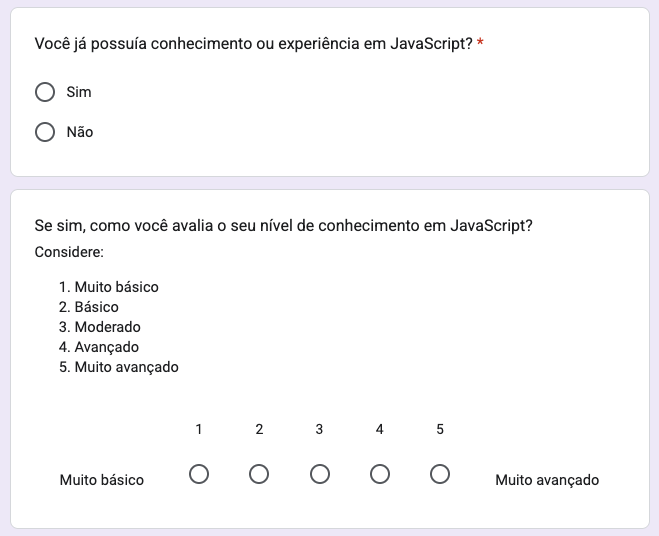
\includegraphics[width=0.95\textwidth]{images/questao1_2_geral.png}}
        \fonte{Elaborado pelo autor}
    \end{minipage}
\end{figure}
\FloatBarrier

\begin{figure}[ht]
    \caption{Questão 3 e 4 do formulário final para todos os participantes}
    \label{fig:questao3_4_geral}
    \centering
    \footnotesize
    \begin{minipage}{.9\textwidth}
        \centering
        \fbox{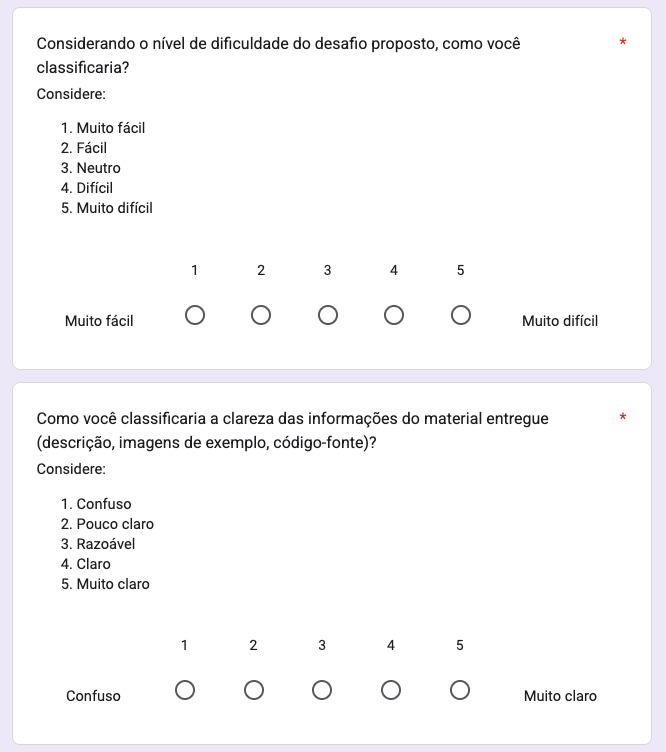
\includegraphics[width=0.95\textwidth]{images/questao3_4_geral.png}}
        \fonte{Elaborado pelo autor}
    \end{minipage}
\end{figure}
\FloatBarrier

\begin{figure}[ht]
    \caption{Questão 5 e 6 do formulário final para todos os participantes}
    \label{fig:questao5_6_geral}
    \centering
    \footnotesize
    \begin{minipage}{.9\textwidth}
        \centering
        \fbox{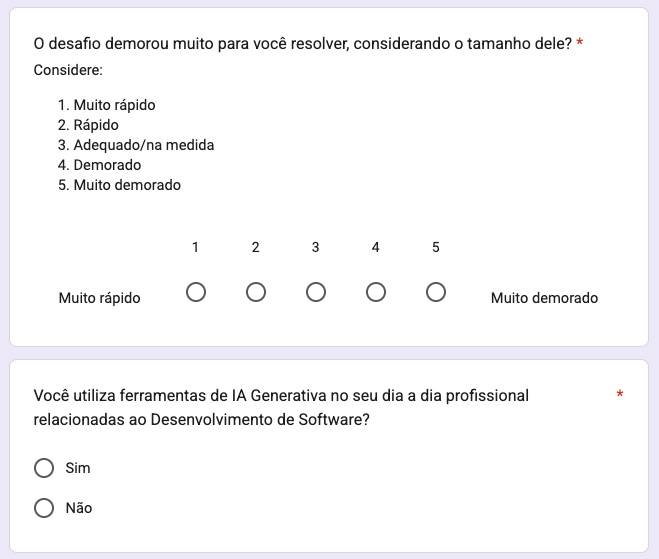
\includegraphics[width=0.95\textwidth]{images/questao5_6_geral.png}}
        \fonte{Elaborado pelo autor}
    \end{minipage}
\end{figure}
\FloatBarrier

\begin{figure}[ht]
    \caption{Questão 7 do formulário final para todos os participantes}
    \label{fig:questao7_geral}
    \centering
    \footnotesize
    \begin{minipage}{.9\textwidth}
        \centering
        \fbox{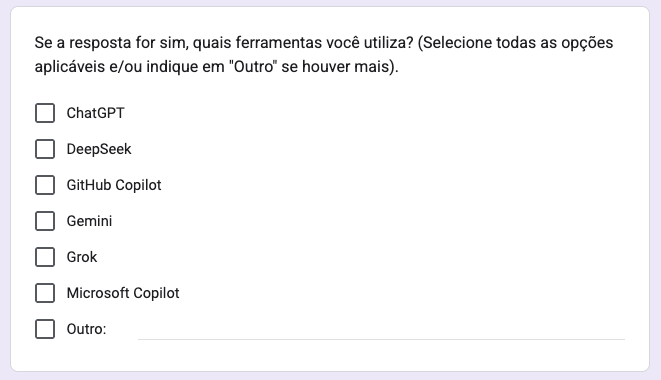
\includegraphics[width=0.95\textwidth]{images/questao7_geral.png}}
        \fonte{Elaborado pelo autor}
    \end{minipage}
\end{figure}
\FloatBarrier

\begin{figure}[ht]
    \caption{Questão 8, 9 e 10 do formulário final para todos os membros do grupo sem IA}
    \label{fig:questao8_9_10_sem_ia}
    \centering
    \footnotesize
    \begin{minipage}{.9\textwidth}
        \centering
        \fbox{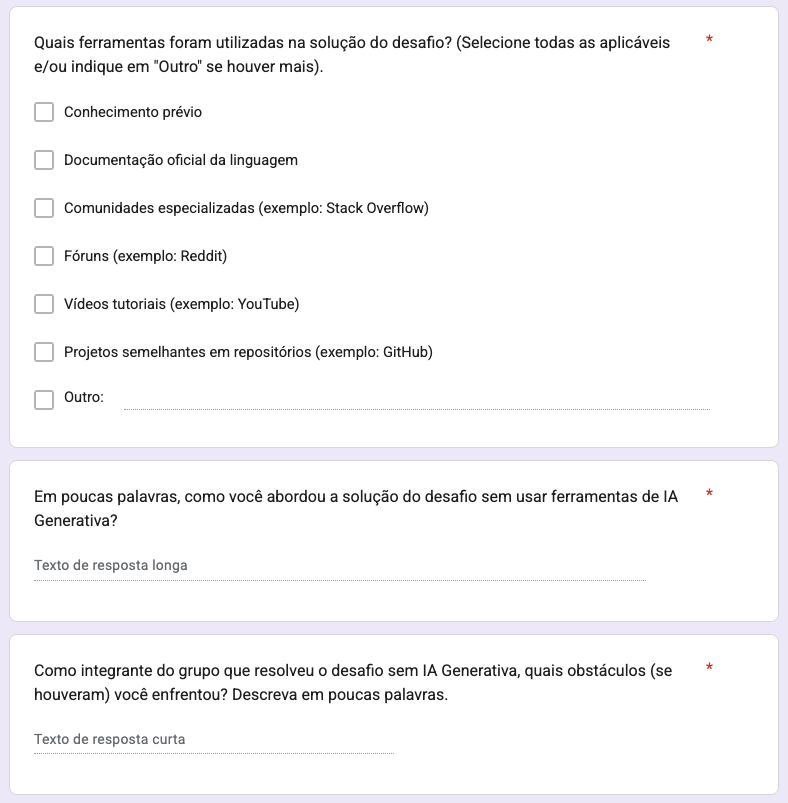
\includegraphics[width=0.95\textwidth]{images/questao8_9_10_sem_ia.png}}
        \fonte{Elaborado pelo autor}
    \end{minipage}
\end{figure}
\FloatBarrier

\begin{figure}[ht]
    \caption{Questão 8, 9 e 10 do formulário final para todos os membros do grupo com IA}
    \label{fig:questao8_9_10_com_ia}
    \centering
    \footnotesize
    \begin{minipage}{.9\textwidth}
        \centering
        \fbox{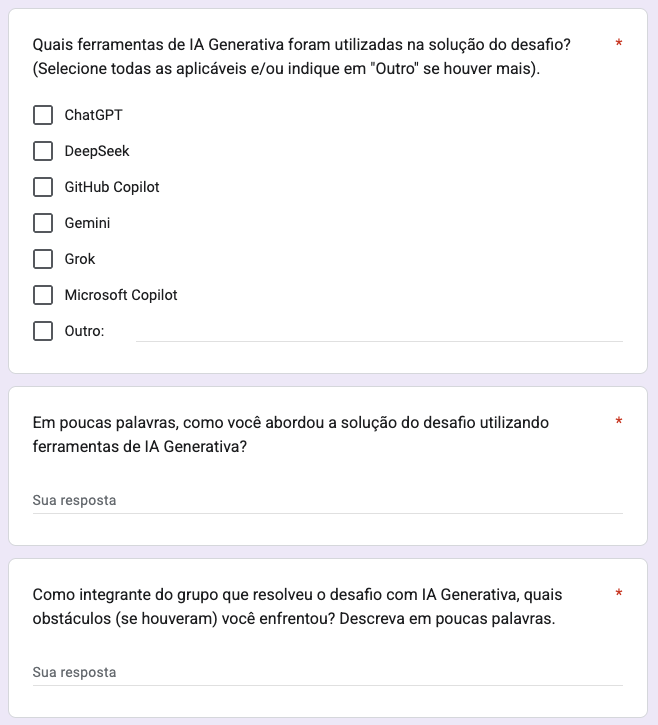
\includegraphics[width=0.95\textwidth]{images/questao8_9_10_com_ia.png}}
        \fonte{Elaborado pelo autor}
    \end{minipage}
\end{figure}
\FloatBarrier

\begin{figure}[ht]
    \caption{Questão 11 do formulário final para todos os participantes}
    \label{fig:questao11_geral}
    \centering
    \footnotesize
    \begin{minipage}{.9\textwidth}
        \centering
        \fbox{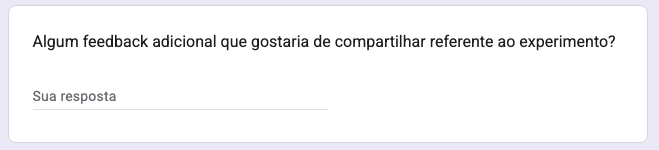
\includegraphics[width=0.95\textwidth]{images/questao11_geral.png}}
        \fonte{Elaborado pelo autor}
    \end{minipage}
\end{figure}
\FloatBarrier

\section{RESPOSTAS DO FORMULÁRIO}

\renewcommand{\thefigure}{F.\arabic{figure}}
\setcounter{figure}{0}

\renewcommand{\thetable}{F.\arabic{table}}
\setcounter{table}{0}

Os gráficos e quadros abaixo representam as respostas completas do questionário, dos grupos sem IA e com IA, respectivamente. Os Gráficos \ref{graf:resposta1_sem_ia} e \ref{graf:resposta1_com_ia} referem-se à questão 1. Os Gráficos \ref{graf:resposta2_sem_ia} e \ref{graf:resposta2_com_ia} são as respostas da questão 2. Os Gráficos \ref{graf:resposta3_sem_ia} e \ref{graf:resposta3_com_ia} referem-se à questão 3. Os Gráficos \ref{graf:resposta4_sem_ia} e \ref{graf:resposta4_com_ia} são da questão 4. Os Gráficos \ref{graf:resposta5_sem_ia} e \ref{graf:resposta5_com_ia} são referentes à questão 5. Os Gráficos \ref{graf:resposta6_sem_ia} e \ref{graf:resposta6_com_ia} tratam-se da questão 6. Os Gráfico \ref{graf:resposta7_sem_ia} e \ref{graf:resposta7_com_ia} referem-se à questão 7. Os Gráficos \ref{graf:resposta8_sem_ia} e \ref{graf:resposta8_com_ia} são as repostas da questão 8.

As Tabelas \ref{tab:questao9_sem_ia} e \ref{tab:questao9_com_ia} referem-se à questão 9. As Tabelas \ref{tab:questao10_sem_ia} e \ref{tab:questao10_com_ia} são as respostas da questão 10. Por fim, as tabelas \ref{tab:questao11_sem_ia} e \ref{tab:questao11_com_ia} tratam-se da questão 11.

\begin{figure}[ht]
    \caption{Respotas da questão 1 de todos do grupo sem IA}
    \label{graf:resposta1_sem_ia}
    \centering
    \footnotesize
    \begin{minipage}{.9\textwidth}
        \centering
        \fbox{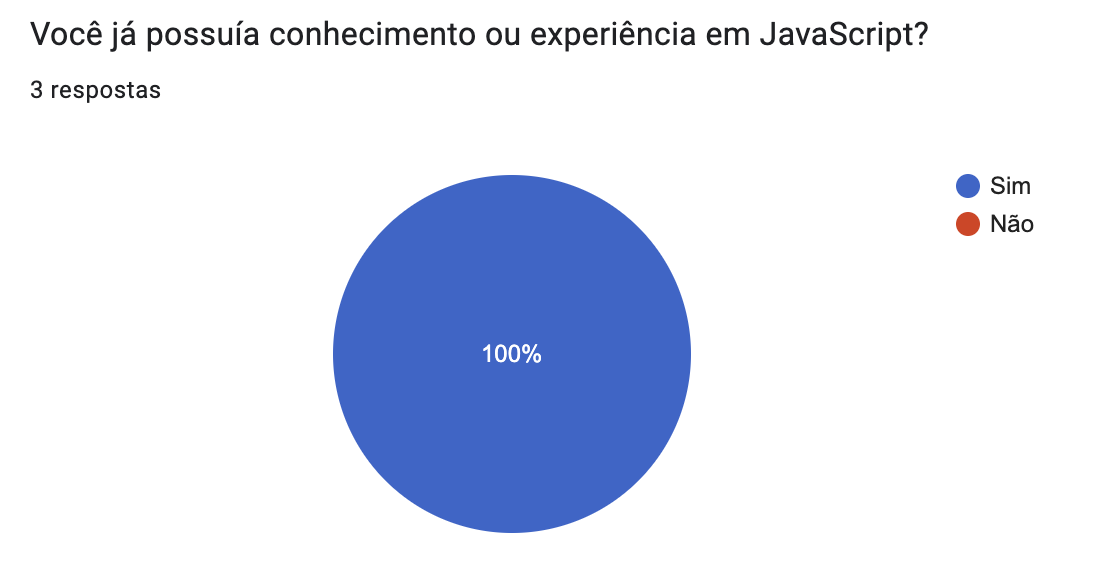
\includegraphics[width=0.95\textwidth]{images/resposta1_sem_com_ia.png}}
        \fonte{Elaborado pelo autor}
    \end{minipage}
\end{figure}
\FloatBarrier

\begin{figure}[ht]
    \caption{Respotas da questão 1 de todos do grupo com IA}
    \label{graf:resposta1_com_ia}
    \centering
    \footnotesize
    \begin{minipage}{.9\textwidth}
        \centering
        \fbox{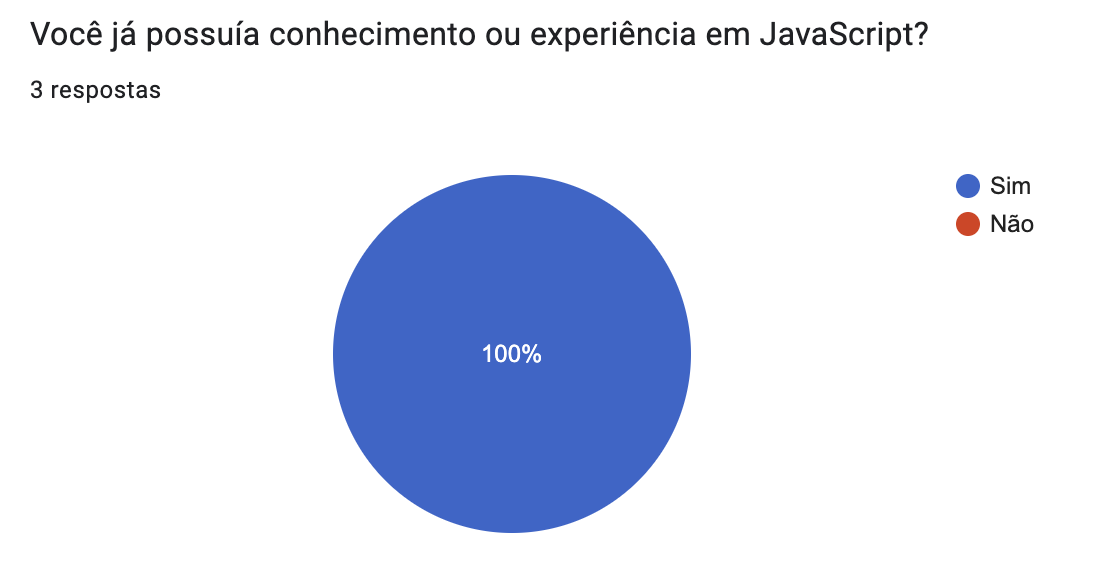
\includegraphics[width=0.95\textwidth]{images/resposta1_sem_com_ia.png}}
        \fonte{Elaborado pelo autor}
    \end{minipage}
\end{figure}
\FloatBarrier

\begin{figure}[ht]
    \caption{Respotas da questão 2 de todos do grupo sem IA}
    \label{graf:resposta2_sem_ia}
    \centering
    \footnotesize
    \begin{minipage}{.9\textwidth}
        \centering
        \fbox{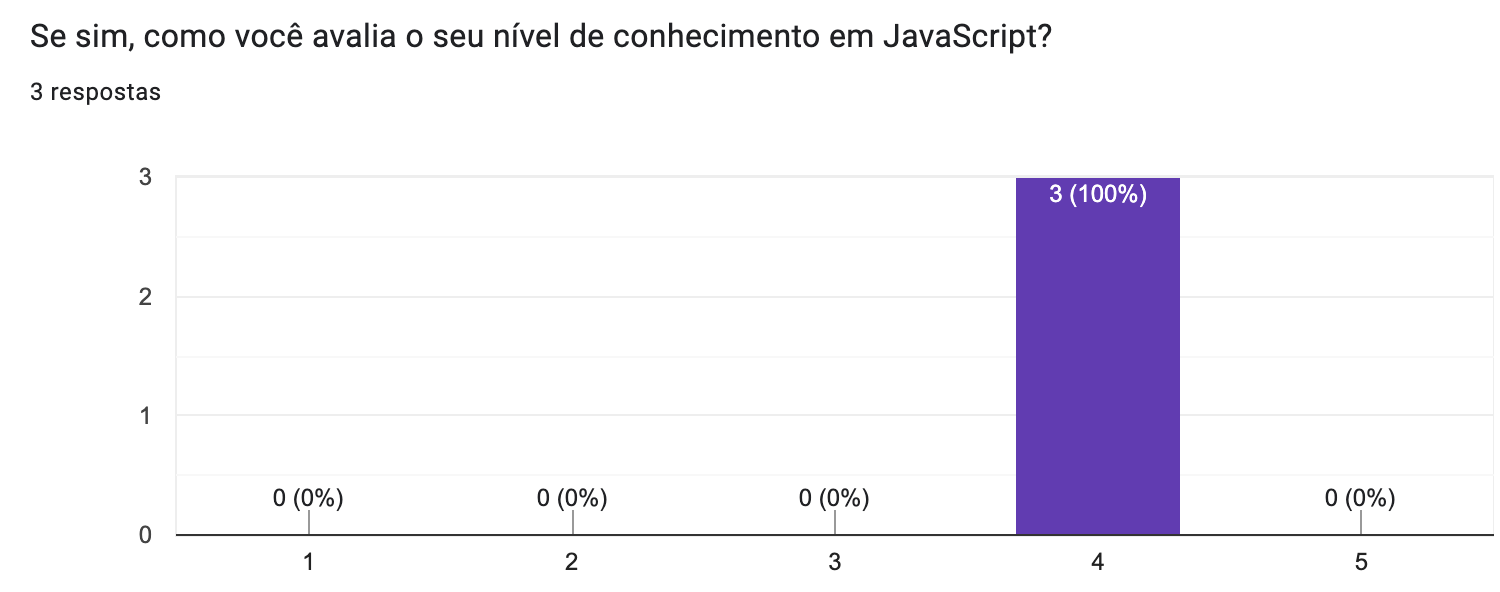
\includegraphics[width=0.95\textwidth]{images/resposta2_sem_ia.png}}
        \fonte{Elaborado pelo autor}
    \end{minipage}
\end{figure}
\FloatBarrier

\begin{figure}[ht]
    \caption{Respotas da questão 2 de todos do grupo com IA}
    \label{graf:resposta2_com_ia}
    \centering
    \footnotesize
    \begin{minipage}{.9\textwidth}
        \centering
        \fbox{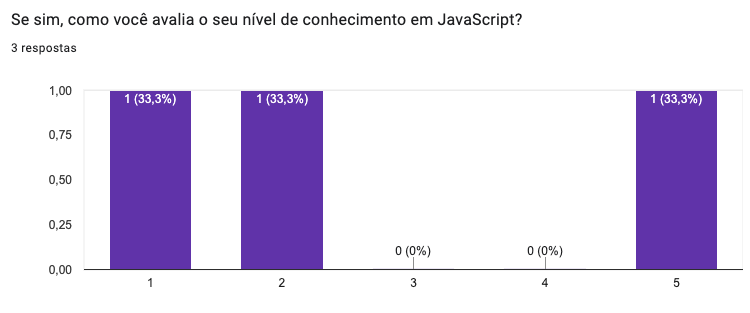
\includegraphics[width=0.95\textwidth]{images/resposta2_com_ia.png}}
        \fonte{Elaborado pelo autor}
    \end{minipage}
\end{figure}
\FloatBarrier

\begin{figure}[ht]
    \caption{Respotas da questão 3 de todos do grupo sem IA}
    \label{graf:resposta3_sem_ia}
    \centering
    \footnotesize
    \begin{minipage}{.9\textwidth}
        \centering
        \fbox{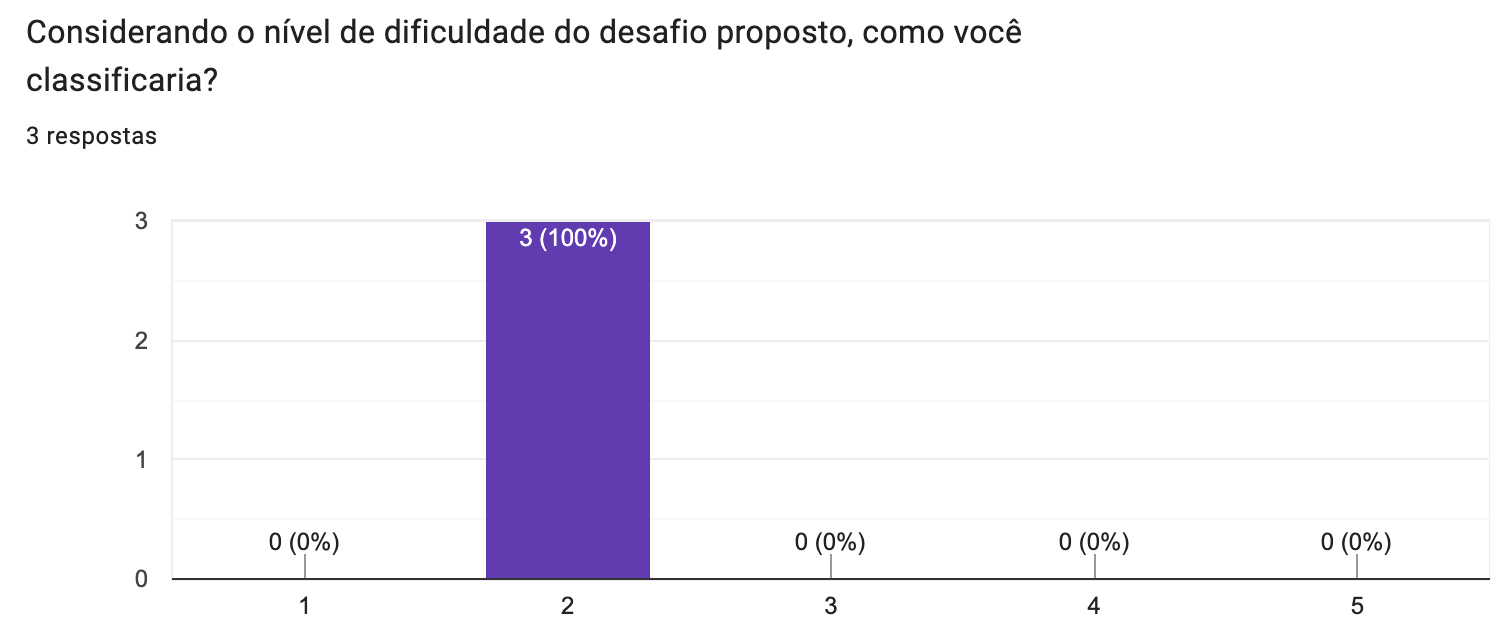
\includegraphics[width=0.95\textwidth]{images/resposta3_sem_ia.png}}
        \fonte{Elaborado pelo autor}
    \end{minipage}
\end{figure}
\FloatBarrier

\begin{figure}[ht]
    \caption{Respotas da questão 3 de todos do grupo com IA}
    \label{graf:resposta3_com_ia}
    \centering
    \footnotesize
    \begin{minipage}{.9\textwidth}
        \centering
        \fbox{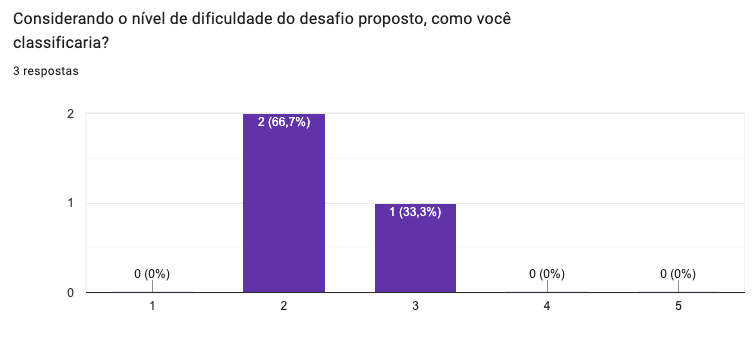
\includegraphics[width=0.95\textwidth]{images/resposta3_com_ia.png}}
        \fonte{Elaborado pelo autor}
    \end{minipage}
\end{figure}
\FloatBarrier

\begin{figure}[ht]
    \caption{Respotas da questão 4 de todos do grupo sem IA}
    \label{graf:resposta4_sem_ia}
    \centering
    \footnotesize
    \begin{minipage}{.9\textwidth}
        \centering
        \fbox{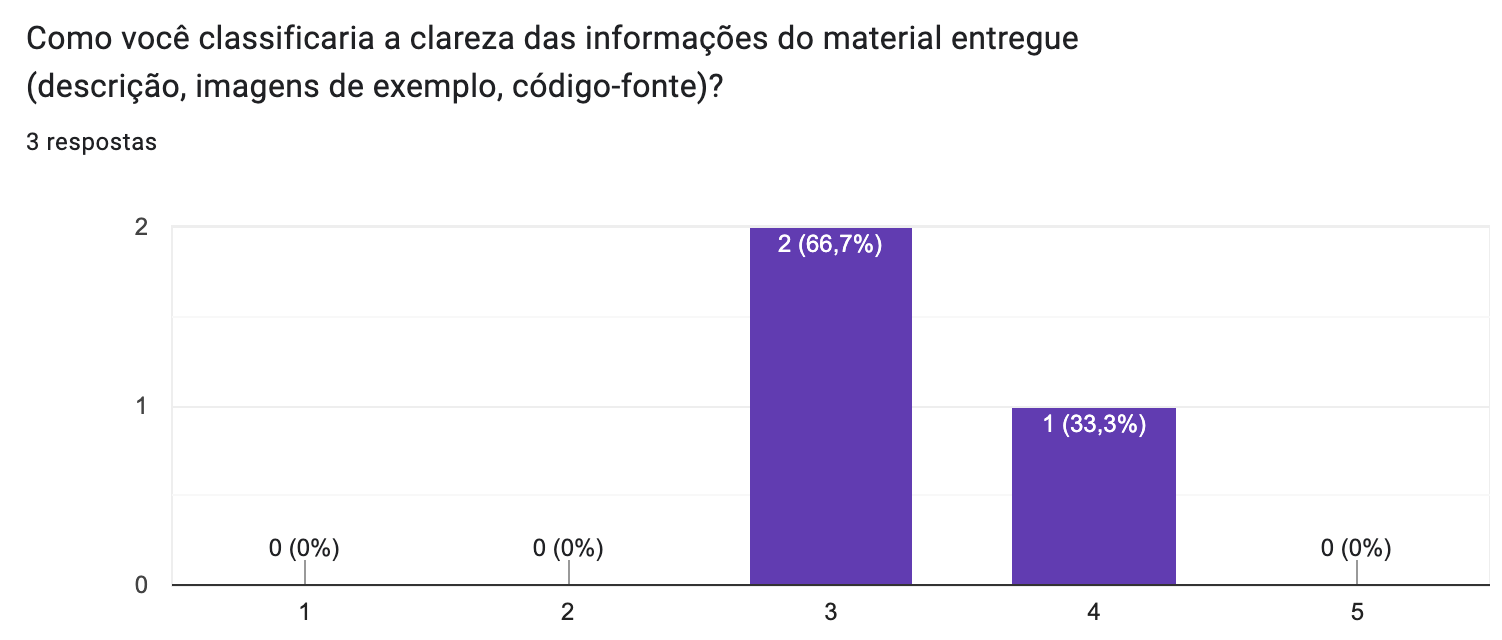
\includegraphics[width=0.95\textwidth]{images/resposta4_sem_ia.png}}
        \fonte{Elaborado pelo autor}
    \end{minipage}
\end{figure}
\FloatBarrier

\begin{figure}[ht]
    \caption{Respotas da questão 4 de todos do grupo com IA}
    \label{graf:resposta4_com_ia}
    \centering
    \footnotesize
    \begin{minipage}{.9\textwidth}
        \centering
        \fbox{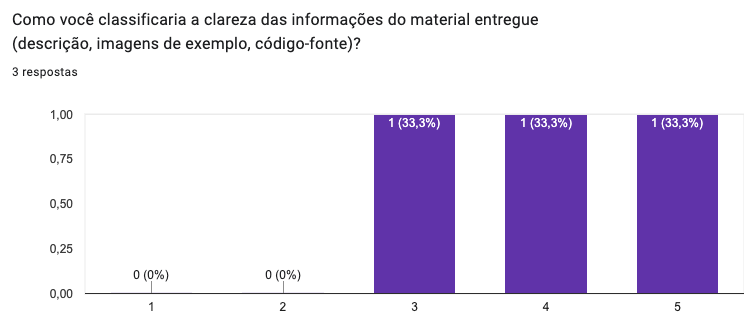
\includegraphics[width=0.95\textwidth]{images/resposta4_com_ia.png}}
        \fonte{Elaborado pelo autor}
    \end{minipage}
\end{figure}
\FloatBarrier

\begin{figure}[ht]
    \caption{Respotas da questão 5 de todos do grupo sem IA}
    \label{graf:resposta5_sem_ia}
    \centering
    \footnotesize
    \begin{minipage}{.9\textwidth}
        \centering
        \fbox{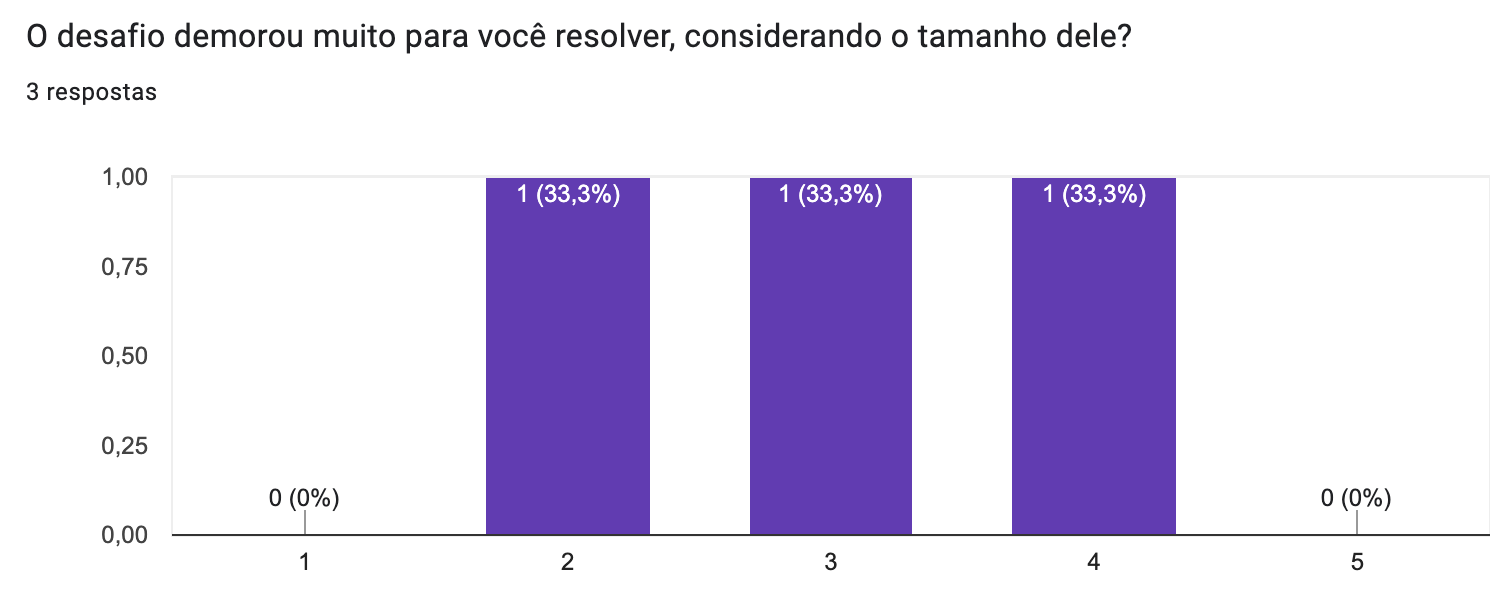
\includegraphics[width=0.95\textwidth]{images/resposta5_sem_ia.png}}
        \fonte{Elaborado pelo autor}
    \end{minipage}
\end{figure}
\FloatBarrier

\begin{figure}[ht]
    \caption{Respotas da questão 5 de todos do grupo com IA}
    \label{graf:resposta5_com_ia}
    \centering
    \footnotesize
    \begin{minipage}{.9\textwidth}
        \centering
        \fbox{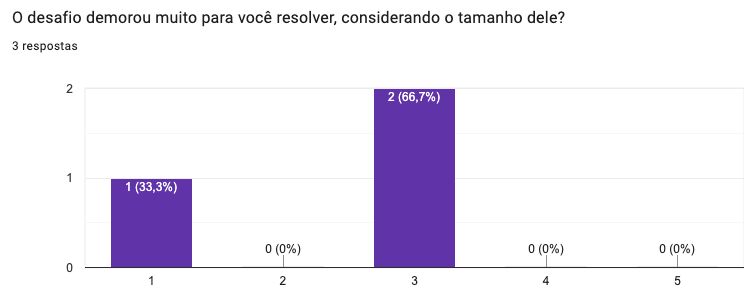
\includegraphics[width=0.95\textwidth]{images/resposta5_com_ia.png}}
        \fonte{Elaborado pelo autor}
    \end{minipage}
\end{figure}
\FloatBarrier

\begin{figure}[ht]
    \caption{Respotas da questão 6 de todos do grupo sem IA}
    \label{graf:resposta6_sem_ia}
    \centering
    \footnotesize
    \begin{minipage}{.9\textwidth}
        \centering
        \fbox{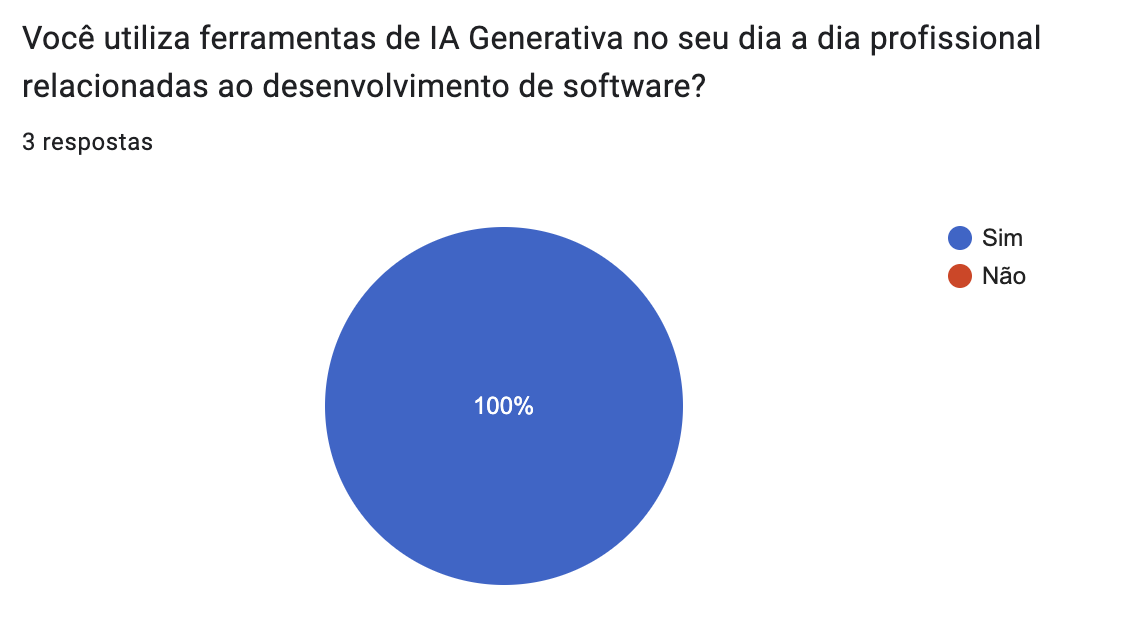
\includegraphics[width=0.95\textwidth]{images/resposta6_sem_com_ia.png}}
        \fonte{Elaborado pelo autor}
    \end{minipage}
\end{figure}
\FloatBarrier

\begin{figure}[ht]
    \caption{Respotas da questão 6 de todos do grupo com IA}
    \label{graf:resposta6_com_ia}
    \centering
    \footnotesize
    \begin{minipage}{.9\textwidth}
        \centering
        \fbox{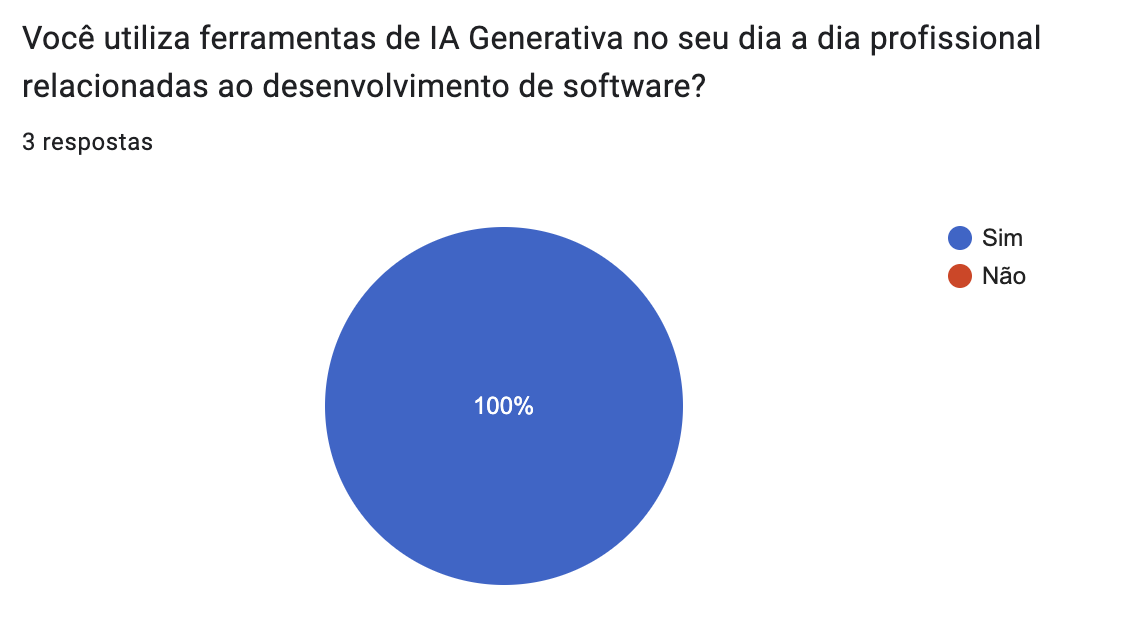
\includegraphics[width=0.95\textwidth]{images/resposta6_sem_com_ia.png}}
        \fonte{Elaborado pelo autor}
    \end{minipage}
\end{figure}
\FloatBarrier

\begin{figure}[ht]
    \caption{Respotas da questão 7 de todos do grupo sem IA}
    \label{graf:resposta7_sem_ia}
    \centering
    \footnotesize
    \begin{minipage}{.9\textwidth}
        \centering
        \fbox{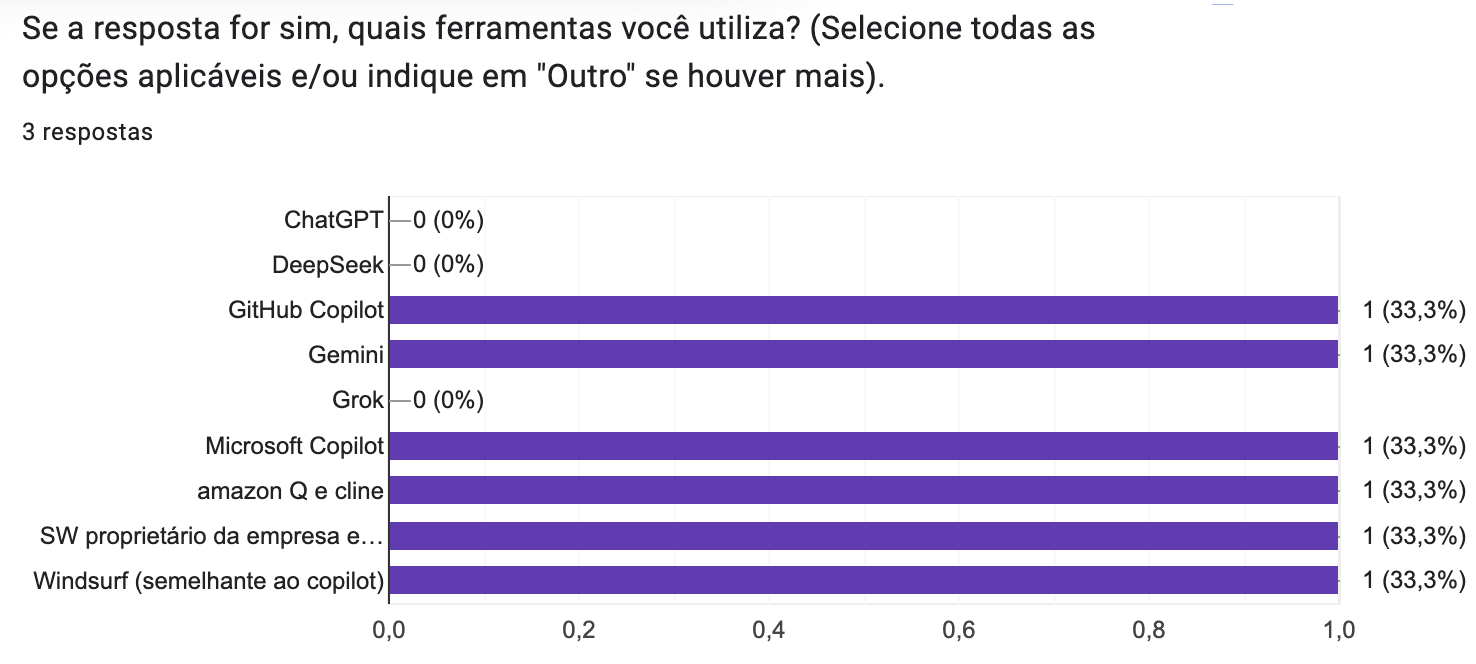
\includegraphics[width=0.95\textwidth]{images/resposta7_sem_ia.png}}
        \fonte{Elaborado pelo autor}
    \end{minipage}
\end{figure}
\FloatBarrier

\begin{figure}[ht]
    \caption{Respotas da questão 7 de todos do grupo com IA}
    \label{graf:resposta7_com_ia}
    \centering
    \footnotesize
    \begin{minipage}{.9\textwidth}
        \centering
        \fbox{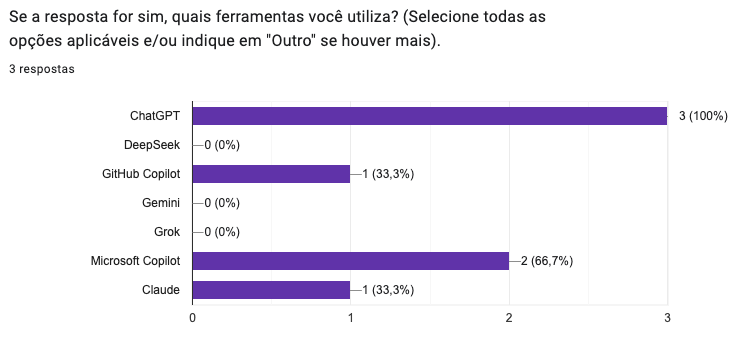
\includegraphics[width=0.95\textwidth]{images/resposta7_com_ia.png}}
        \fonte{Elaborado pelo autor}
    \end{minipage}
\end{figure}
\FloatBarrier

\begin{figure}[ht]
    \caption{Respotas da questão 8 de todos do grupo sem IA}
    \label{graf:resposta8_sem_ia}
    \centering
    \footnotesize
    \begin{minipage}{.9\textwidth}
        \centering
        \fbox{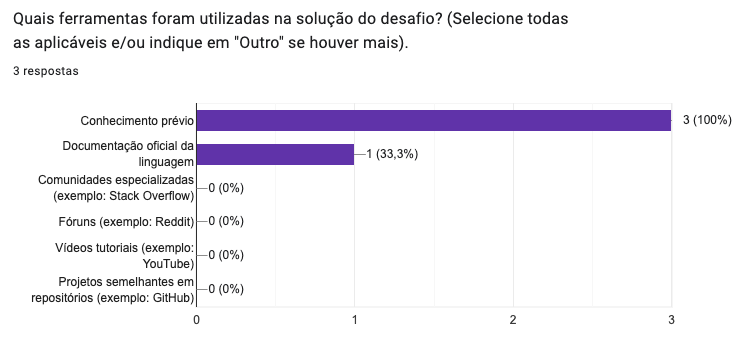
\includegraphics[width=0.95\textwidth]{images/resposta8_sem_ia.png}}
        \fonte{Elaborado pelo autor}
    \end{minipage}
\end{figure}
\FloatBarrier

\begin{figure}[ht]
    \caption{Respotas da questão 8 de todos do grupo com IA}
    \label{graf:resposta8_com_ia}
    \centering
    \footnotesize
    \begin{minipage}{.9\textwidth}
        \centering
        \fbox{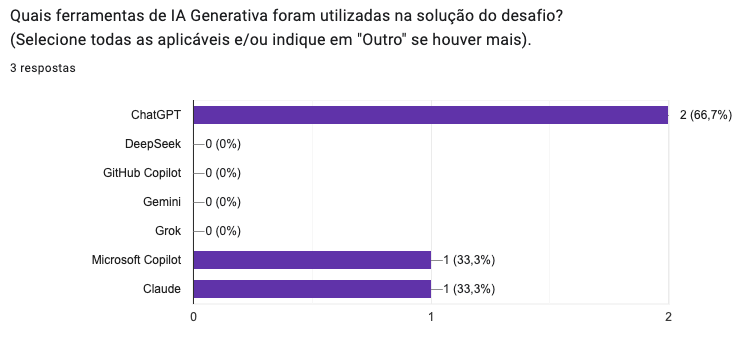
\includegraphics[width=0.95\textwidth]{images/resposta8_com_ia.png}}
        \fonte{Elaborado pelo autor}
    \end{minipage}
\end{figure}
\FloatBarrier

\begin{table}[ht]
    \caption{Respostas da questão 9 de todos do grupo sem IA}
    \label{tab:questao9_sem_ia}
    \centering%
    \footnotesize
    \begin{tabularx}{\textwidth}{lXXXX}
        \toprule
        \textbf{Participante} & \textbf{Em poucas palavras, como você abordou a solução do desafio sem usar ferramentas de IA Generativa?} \\
        \midrule
        Desenvolvedor 1 & Primeiramente, tentei achar os bugs. Para isso, explorei a aplicação já pronta. Tendo isso em vista, fui encontrando a raiz dos problemas e resolvendo. Usei o debugger do navegador para entender quais os problemas com os dados. \\
        \midrule
        Desenvolvedor 2 & Realizei alguns testes e verifiquei o resultado final. A partir daí analisei o código e ajustei conforme fui debugando. \\
        \midrule
        Desenvolvedor 3 & Fui analisando os resultados e revisando o código no VSCode conforme eu encontrava os erros neles \\
        \bottomrule
    \end{tabularx}
    \fonte{Elaborado pelo autor}
\end{table}
\FloatBarrier

\begin{table}[ht]
    \caption{Respostas da questão 9 de todos do grupo com IA}
    \label{tab:questao9_com_ia}
    \centering%
    \footnotesize
    \begin{tabularx}{\textwidth}{lXXXX}
        \toprule
        \textbf{Participante} & \textbf{Em poucas palavras, como você abordou a solução do desafio sem usar ferramentas de IA Generativa?} \\
        \midrule
        Desenvolvedor 4 & Basicamente copiou os prints de output esperados e a descrição do desafio. \\
        \midrule
        Desenvolvedor 5 & Me fiz de leigo. Mandei a IA ler todo o projeto, onde ela ja encontrou e corrigiu bugs, e depois mandei o deafio e pedi pra ele ajustar o projeto de acordo. No final, pedi pra ele testar e me mandar evidencias que está correto. No final, fiz testes exploratorios manuais e entreguei o projeto. \\
        \midrule
        Desenvolvedor 6 & De início eu tentei fazer tudo sozinho, baseado na leitura do código e outputs do programa. Mas, depois de acreditar ter resolvido tudo e ainda assim ver alguns bugs, submeti o código inteiro ao chatGPT, que prontamente já me sugeriu alguns fixes antes de eu pedir qualquer coisa.

        Após isso, somente um bug sobrou, onde agora submeti o input e falei "o resultado atual está errado", e ele prontamente me deu os fixes novamente. \\
        \bottomrule
    \end{tabularx}
    \fonte{Elaborado pelo autor}
\end{table}
\FloatBarrier

\begin{table}[ht]
    \caption{Respostas da questão 10 de todos do grupo sem IA}
    \label{tab:questao10_sem_ia}
    \centering%
    \footnotesize
    \begin{tabularx}{\textwidth}{lXXXX}
        \toprule
        \textbf{Participante} & \textbf{Como integrante do grupo que resolveu o desafio sem IA Generativa, quais obstáculos (se houveram) você enfrentou? Descreva em poucas palavras.} \\
        \midrule
        Desenvolvedor 1 & Encontrar os bugs em si. \\
        \midrule
        Desenvolvedor 2 & Senti falta do autocomplete fornecido pelo windsurf, já que utilizo bastante para tarefas mais manuais. \\
        \midrule
        Desenvolvedor 3 & A pesquisa por informações e a revisão de código tornam-se muito mais demoradas e complicadas sem o uso de IA. \\
        \bottomrule
    \end{tabularx}
    \fonte{Elaborado pelo autor}
\end{table}
\FloatBarrier

\begin{table}[ht]
    \caption{Respostas da questão 10 de todos do grupo com IA}
    \label{tab:questao10_com_ia}
    \centering%
    \footnotesize
    \begin{tabularx}{\textwidth}{lXXXX}
        \toprule
        \textbf{Participante} & \textbf{Como integrante do grupo que resolveu o desafio com IA Generativa, quais obstáculos (se houveram) você enfrentou? Descreva em poucas palavras.} \\
        \midrule
        Desenvolvedor 4 & chatgpt free, tem um limite muito pequeno de entradas, tive que ir para o Copilot \\
        \midrule
        Desenvolvedor 5 & Nenhum. \\
        \midrule
        Desenvolvedor 6 & Com IA, nenhum. \\
        \bottomrule
    \end{tabularx}
    \fonte{Elaborado pelo autor}
\end{table}
\FloatBarrier

\begin{table}[ht]
    \caption{Respostas da questão 11 de todos do grupo sem IA}
    \label{tab:questao11_sem_ia}
    \centering%
    \footnotesize
    \begin{tabularx}{\textwidth}{lXXXX}
        \toprule
        \textbf{Participante} & \textbf{Algum feedback adicional que gostaria de compartilhar referente ao experimento?} \\
        \midrule
        Desenvolvedor 2 & Faltou ser um pouco mais claro na descrição do problema \\
        \midrule
        Desenvolvedor 3 & Interessante notar como a IA se tornou uma ferramenta tão importante no meu processo de desenvolvimento. Antes do experimente eu poderia dizer que fácilmente conseguiria desenvolver sem o uso de IA mas após ele consigo notar que o processo se torna muito mais demorado sem o uso da mesma. \\
        \bottomrule
    \end{tabularx}
    \fonte{Elaborado pelo autor}
\end{table}
\FloatBarrier

\begin{table}[ht]
    \caption{Respostas da questão 11 de todos do grupo com IA}
    \label{tab:questao11_com_ia}
    \centering%
    \footnotesize
    \begin{tabularx}{\textwidth}{lXXXX}
        \toprule
        \textbf{Participante} & \textbf{Algum feedback adicional que gostaria de compartilhar referente ao experimento?} \\
        \midrule
        Desenvolvedor 6 & seria muito mais simples se nas instruções não houvessem prints da tela, mas sim textos de input e output, pra que a gente copiasse e colasse, invés de ter que ler a imagem e copiar. \\
        \bottomrule
    \end{tabularx}
    \fonte{Elaborado pelo autor}
\end{table}
\FloatBarrier

\section{CÓDIGO-FONTE BASE E CÓDIGO-FONTE DO DESAFIO}

\renewcommand{\thelstlisting}{G.\arabic{lstlisting}}

\lstinputlisting[caption={Código-fonte base do Desafio Técnico}]{source_code/main_base.js}

\lstinputlisting[caption={Código-fonte do Desafio Técnico}]{source_code/main.js}

\section{LISTA DE \textit{BUGS} E ANÁLISES DOS DESENVOLVEDORES}

\renewcommand{\thefigure}{H.\arabic{figure}}
\setcounter{figure}{0}

\begin{figure}[ht]
    \caption{Lista de \textit{bugs} implementados no arquivo \texttt{main.js}}
    \label{fig:bugs}
    \centering
    \footnotesize
    \begin{minipage}{.9\textwidth}
        \centering
        \fbox{\includegraphics[width=1\textwidth]{images/bugs.png}}
        \fonte{Elaborado pelo autor}
    \end{minipage}
\end{figure}
\FloatBarrier

\begin{figure}[ht]
    \caption{Análises dos desenvolvedores do grupo sem IA}
    \label{fig:resultados_bugs_sem_ia}
    \centering
    \footnotesize
    \begin{minipage}{.9\textwidth}
        \centering
        \fbox{\includegraphics[width=1\textwidth]{images/resultados_bugs_sem_ia.png}}
        \fonte{Elaborado pelo autor}
    \end{minipage}
\end{figure}
\FloatBarrier

\begin{figure}[ht]
    \caption{Análises dos desenvolvedores do grupo com IA}
    \label{fig:resultados_bugs_com_ia}
    \centering
    \footnotesize
    \begin{minipage}{.9\textwidth}
        \centering
        \fbox{\includegraphics[width=1\textwidth]{images/resultados_bugs_com_ia.png}}
        \fonte{Elaborado pelo autor}
    \end{minipage}
\end{figure}
\FloatBarrier

\end{document}
